\pdfoutput=1
%\documentclass[gray]{jmlr} % test grayscale version
%\documentclass[tablecaption=bottom]{jmlr}% journal article
\documentclass[pmlr,twocolumn,10pt]{jmlr} % W&CP article

% The following packages will be automatically loaded:
% amsmath, amssymb, natbib, graphicx, url, algorithm2e

%\usepackage{rotating}% for sideways figures and tables
%\usepackage{longtable}% for long tables

% The booktabs package is used by this sample document
% (it provides \toprule, \midrule and \bottomrule).
% Remove the next line if you don't require it.

\usepackage{booktabs}
% The siunitx package is used by this sample document
% to align numbers in a column by their decimal point.
% Remove the next line if you don't require it.
%\usepackage[load-configurations=version-1]{siunitx} % newer version 
\usepackage{siunitx}

% The lineno package is required for denoting line
% numbers for paper review.
\usepackage[switch]{lineno}

\usepackage{url}
\def\UrlBreaks{\do\/\do-}

% The following is to recognise equal contribution for authorship
\newcommand{\equal}[1]{{\hypersetup{linkcolor=black}\thanks{#1}}}

\newcommand{\MY}[1]{\textcolor{blue}{(Mengyue: #1)}}
\newcommand{\KZ}[1]{\textcolor{red}{(Kenny: #1)}}
\newcommand{\DI}[1]{\textcolor{orange}{(Dilawaier: #1)}}
\newcommand{\WY}[1]{\textcolor{green}{(Weiye: #1)}}
\newcommand{\secref}[1]{Sec. \ref{#1}}
\newcommand{\figref}[1]{Figure \ref{#1}}
\newcommand{\eqnref}[1]{Eq. (\ref{#1})}
\newcommand{\tabref}[1]{Table \ref{#1}}
\newcommand{\exref}[1]{Example \ref{#1}}

% Define an unnumbered theorem just for this sample document for
% illustrative purposes:
\theorembodyfont{\upshape}
\theoremheaderfont{\scshape}
\theorempostheader{:}
\theoremsep{\newline}
\newtheorem*{note}{Note}

% change the arguments, as appropriate, in the following:
\jmlrvolume{LEAVE UNSET}
\jmlryear{2024}
\jmlrsubmitted{LEAVE UNSET}
\jmlrpublished{LEAVE UNSET}
\jmlrworkshop{Conference on Health, Inference, and Learning (CHIL) 2024} % W&CP title

% The optional argument of \title is used in the header
\title[PsyEval]{PsyEval: A Comprehensive Large Language Model\titlebreak
Evaluation Benchmark for Mental Health}

% \author{Haoan Jin\textsuperscript{1}, Siyuan Chen\textsuperscript{1}, Dilawaier Dilixiati\textsuperscript{2}, Jiang Yewei\textsuperscript{2}, Mengyue Wu\textsuperscript{1}, Kenny Q. Zhu\textsuperscript{3} \\
%   \textsuperscript{1}X-LANCE LAB, Shanghai Jiao Tong University, Shanghai, China \\
%   \textsuperscript{2}Shanghai Jiao Tong University School of Medicine, Shanghai, China \\
%   \textsuperscript{3}University of Texas at Arlington, Arlington, Texas, USA \\
%   \texttt{\{pilgrim, chensiyuan925, mengyuewu\}@sjtu.edu.cn}\\
%   \texttt{\{dilawur1, zoe8188\}@sjtu.edu.cn}\\
%   \texttt{kenny.zhu@uta.edu} \\}


% Anything in the title that should appear in the main title but 
% not in the article's header or the volume's table of
% contents should be placed inside \titletag{}

%\title{Title of the Article\titletag{\thanks{Some footnote}}}


% Use \Name{Author Name} to specify the name.
% If the surname contains spaces, enclose the surname
% in braces, e.g. \Name{John {Smith Jones}} similarly
% if the name has a "von" part, e.g \Name{Jane {de Winter}}.
% If the first letter in the forenames is a diacritic
% enclose the diacritic in braces, e.g. \Name{{\'E}louise Smith}

% \thanks must come after \Name{...} not inside the argument for
% example \Name{John Smith}\nametag{\thanks{A note}} NOT \Name{John
% Smith\thanks{A note}}

% Anything in the name that should appear in the title but not in the 
% article's header or footer or in the volume's
% table of contents should be placed inside \nametag{}

% Two authors with the same address
% \author{%
%  \Name{Author Name1\nametag{\thanks{A note}}} \Email{abc@sample.com}\and
%  \Name{Author Name2} \Email{xyz@sample.com}\\
%  \addr Address
% }

% Three or more authors with the same address:
% \author{%
%  \Name{Author Name1} \Email{an1@sample.com}\\
%  \Name{Author Name2} \Email{an2@sample.com}\\
%  \Name{Author Name3} \Email{an3@sample.com}\\
%  \Name{Author Name4} \Email{an4@sample.com}\\
%  \Name{Author Name5} \Email{an5@sample.com}\\
%  \Name{Author Name6} \Email{an6@sample.com}\\
%  \Name{Author Name7} \Email{an7@sample.com}\\
%  \Name{Author Name8} \Email{an8@sample.com}\\
%  \Name{Author Name9} \Email{an9@sample.com}\\
%  \Name{Author Name10} \Email{an10@sample.com}\\
%  \Name{Author Name11} \Email{an11@sample.com}\\
%  \Name{Author Name12} \Email{an12@sample.com}\\
%  \Name{Author Name13} \Email{an13@sample.com}\\
%  \Name{Author Name14} \Email{an14@sample.com}\\
%  \addr Address
% }

% \author{
% \Name{Haoan Jin} \Email{pilgrim@sjtu.edu.cn}\\
% \addr Shanghai Jiao Tong University, China\\
% \AND
% \Name{Siyuan Chen} \Email{chensiyuan925@sjtu.edu.cn}\\
% \addr Shanghai Jiao Tong University, China\\
% \AND
% \Name{Dilawaier Dilixiati} \Email{dilawur1@sjtu.edu.cn}\\
% \addr Shanghai Jiao Tong University School of Medicine, China\\
% \AND
% \Name{Yewei Jiang} \Email{zoe8188@sjtu.edu.cn}\\
% \addr Shanghai Jiao Tong University School of Medicine, China\\
% \AND
% \Name{Mengyue Wu} \Email{mengyuewu@sjtu.edu.cn}\\
% \addr Shanghai Jiao Tong University, China
% \AND
% \Name{Kenny Q. Zhu} \Email{kenny.zhu@uta.edu}\\
% \addr University of Texas at Arlington, USA
% }

\author{
\Name{Anonymous First Author 1}\Email{abc@sample.com}\\
\addr University X, Country 1
}

%%%%%%%%%%%%%%%%%%%%%%%%%%%%%%%%%%%%%%%%%%%%%%%%%%%%%%%%%%%%%%%%%%%%%%%%
%%%%%%%%%%%%% Remove the \linenumbers in the final version %%%%%%%%%%%%%
%%%%%%%%%%%%%%%%%%%%%%%%%%%%%%%%%%%%%%%%%%%%%%%%%%%%%%%%%%%%%%%%%%%%%%%%
\linenumbers % Activate line numbering

\begin{document}

\maketitle

\begin{abstract}
%Recently, there has been a growing interest in utilizing large language models (LLMs) in mental health research, with studies showcasing their remarkable capabilities, such as disease detection. 
%However, there is currently a lack of a comprehensive benchmark for evaluating the capability of LLMs in this domain. Therefore, we address this gap by 
%\MY{add 1-2sentences from intro, say that why LLM in mental health is important and different from previous tasks.}
Distinguishing mental health from other domains, the evaluation of Large Language Model (LLMs) in mental health demands a nuanced approach, given the subtle and highly subjective nature of symptoms that exhibit significant variability among individuals. This paper presents the first comprehensive benchmark for evaluating LLMs in the mental health domain. 
%tailored to the unique characteristics of the mental health domain. 
It encompasses a total of four sub-tasks, covering three dimensions.
%systematically assess the capabilities of LLMs in the realm of mental health. 
We have designed corresponding concise prompts for each sub-task. 
We evaluate a total of twelve advanced LLMs using this benchmark. 
Experiment results not only demonstrate significant room for improvement in current LLMs concerning mental health but also unveil potential directions for future model optimization.
\end{abstract}

\paragraph*{Data and Code Availability}
The data utilized in this study, along with relevant citations where applicable, are made accessible to fellow researchers. Both USMLE-mental and Crisis Response QA have been open-sourced.\footnote{https://anonymous.4open.science/r/Psy-Eval-6A6E}
%\MY{add a footnote and an anonymous github link, saying that the full dataset and experimental details are open-sourced.}

\paragraph*{Institutional Review Board (IRB)}
Due to our human evaluation in the research does not have any adverse effects on the participants' physical or mental well-being, our research does not require IRB approval.

%\IEEEraisesectionheading{
% %\IEEEraisesectionheading{
% %\IEEEraisesectionheading{
% \input{intro}
\section{Introduction}\label{sec:intro}
 %}
% \section{Introduction}\label{sec:intro}

% \begin{enumerate}
% \item Motivation: application scenarios (with 1-2 running examples);
% \item Characteristics of the data sources and their challenges;
% \item Briefly introduce previous approaches to extract information 
% from images including setting the document zone, and their limitations.
% \item General flow of our approach (may give a diagram here)
% \end{enumerate}
% scenary

Due to ever evolving hardware and software, many medical images
such as electro-cardio graphs (ECGs), X-ray or ultrasound images  
are directly printed and stored in hard copy formats. 
% \KZ{Insert 4 example images here.}
%Examples are shown in \figref{fig:medicalImages}. 
% These images often contain a mix of graphics and text, which
% include parameter settings of the hardware, test measurements or simple
% diagnosis. 
These images often contain a mix of graphics and text, which 
include technical settings of the hardware used, test measurements or simple diagnoses.
Recently, there has been a growing demand for digitizing such 
medical information from paper media sources, especially legacy ones, or patients who want to keep track of these documents by themselves digitally. 
Apart from scanning the graphics into a digital format, extracting 
the semi-structured textual information is also an important part of
building electronic medical records for patients. 

%\begin{figure}[!htb]
%\centering
%\subfloat[ECG]{
%\label{fig:medicalimage:ecg}
%\epsfig{file=figure/17_ori.eps, width=0.4\columnwidth}
%}
%% \hfill
%\subfloat[MRI]{
%	\label{fig:medicalimage:mrt}
%	\epsfig{file=figure/MRI.eps, width=0.4\columnwidth}
%}
%\\
%\subfloat[X-RAY]{
%\label{fig:medicalimage:xray}
%\epsfig{file=figure/X-RAY.eps, width=0.4\columnwidth}
%}
%%\hfill
%\subfloat[EEG]{
%\label{fig:medicalimage:eeg}
%\epsfig{file=figure/EEG.eps, width=0.4\columnwidth}
%}
%\caption{Examples of Medical Images}
%\label{fig:medicalImages}
%\end{figure}

Optical character recognition (OCR)  \cite{mori1992historical,smith2007overview} is 
a traditional technique used to turn images of printed text into machine encoded
text. It is well researched and performs well on plain text 
documents such as novels and reports, for a variety of languages. 
%For example, Tesseract, which is one of 
%the most popular open source multilingual recognizers, logs an error 
%rate of 3.72\% for English words and 3.77\% for simplified 
%Chinese characters\cite{smith2009adapting}. 
%Google Books \cite{googlebooks} and Gutenberg \cite{gutenberg} are
%projects which have scanned a large number of paper books into text for free and open
%access. These projects made exclusive use of OCR for this conversion and 
%achieved high accuracy \cite{vincent2007google} \cite{lebert2008project}. 
% 99\% for Gutenberg project \cite{lebert2008project}. 
% \KZ{Give the accuracy of google and gutenberg if available.}


\begin{figure}[th]
\centering
\epsfig{file=figure/17_b.eps, width=0.8\columnwidth}
\caption{An ECG image with text area (red circle) of interest.}
\label{fig:ecgexample2}
\end{figure}

For a semi-structured medical image, such as 
\figref{fig:ecgexample2}, we would like to extract the attribute-value 
pairs (e.g., {\em Vent. rate = 63 bpm}) and possibly other values such as
date ({\em 18-Nov-2010}) and time ({\em 9:13:02}) since those values endow us with lots of information about the patient. 
Existing OCR software cannot extract such structured information in a straightforward 
fashion, 
but instead it produces rather convoluted results from the whole image, 
similar to those in \figref{fig:ocrre}, which was produced by Tesseract, 
a popular multi-lingual recognizers. 
% \KZ{Maybe include the x-y coordinate info in the output as well?}  

\begin{figure}[th]
\centering
\scriptsize
\begin{verbatim}
<p class="ocr_par" title="box 263 33 444 119">
   <span class="ocr_l" title="box 264 33 336 45">
       <span class="ocrx_w" title="box 264 33 299 45">Vcnt.</span> 
       <span class="ocrx_w" title="box 308 34 336 45">rule</span> 
   </span>
   <span class='ocr_l'>
       <span class="ocrx_w" title="box 264 51 283 64">PR</span> 
       <span class="ocrx_w" title="box 291 51 346 64">Interval</span> 
       <span class="ocrx_w" title="box 389 52 411 64">140</span> 
       <span class="ocrx_w" title="box 420 55 439 64">ms</span> 
   </span>
   ...
   </span>
</p>
<p class="ocr_p" dir="ltr">
   <span class="ocr_l">
       <span class="ocrx_w" title="box 396 33 411 45">53</span> 
       <span class="ocrx_w" title="box 420 33 449 48">bpm</span> 
   </span>
</p>
\end{verbatim}
\caption{Snippet OCR results in XML, input to our framework.}
\label{fig:ocrre}
\end{figure}


%\input{xmlre1}

%However, OCR alone does not work well on semi-structured text and hence
%can't be directly used for information extraction from the aforementioned
%medical images. \KZ{Give the reason here, perhaps because OCR models are
%largely Markov based? So semi-structured data breaks the flow of text.}
%When a medical image is input to an ordinary OCR software, the spatial 
%information of the text components is often lost or mixed with noises
%and errors.
%%The reason is OCR converts the whole images into text data, in which 
%%useful information often mix with noises and errors. 
%In this paper, we would like to extract the attribute-value pairs
%and possibly other values from \figref{fig:ecgexample1} 
%and \figref{fig:ecgexample2}. 
%% or medical ultrasonography report. 
%Such images contain lots of non-textual information or noises.

% example & ref
%\begin{figure}[ht]
%\centering
%\epsfig{file=figure/46.eps, width=0.8\columnwidth}
%\caption{ECG Images From Printer1}
%\label{fig:ecgexample1}
%\end{figure}

% \begin{figure}[ht]
% \centering
% \subfloat[Printer1]{
% \label{fig:ecgexample:a}
% \epsfig{file=figure/46.eps, width=0.48\columnwidth}
% }
% \hfill
% \subfloat[Printer2]{
% \label{fig:ecgexample:b}
% \epsfig{file=figure/17.eps, width=0.48\columnwidth}
% }
% \caption{ECG images from two different printers}
% \label{fig:ecgexample}
% \end{figure}

Also, errors in the OCR text \cite{darwish2007error,taghva1996evaluation} will greatly affect the effectiveness 
of other related tasks. Much work has been done to improve the performance of the OCR\cite{kolak2003generative,cesarini1998informys}. However, there are still a number of significant challenges involved in extracting the information from medical images or OCR results in XML form. 

% First, medical images differ from pure text document in that them have 
% layout information. 
First, medical images differ from pure text documents in that 
they contain layout information.
Although most current OCR engines attempt to reproduce the physical 
layout of the text units, 
%(along with X-Y coordinates) and store them 
%in a special format such as XML 
% (\KZ{Better in the previous example})
such spatial
information is approximate and sometimes inaccurate, which is why neighboring
text blocks in \figref{fig:ecgexample2}, such as ``Vent. Rate'' and
``63 bpm'' were not automatically combined into the same XML block, but were 
rather far apart (shown in two different ``classes'') in \figref{fig:ocrre} made by OCR softwares. 
%Even for images produced by the same ECG printer, 
%the XML results can still be very different as 
The spatial layout is sensitive to many factors, such as accidental spots 
on the prints, color and contrast, or the angle of the camera. 
%In this case, solutions for other application domains, for example, the web, 
%are not well suited for information extraction from printed documents \cite{bartoli2014semisupervised}. With such inaccurate
%layout information produced by OCR,
%it is not easy to write a simple wrapper program to extract useful
%data from images, even if the images come from the same printer. 

%Writing a wrapper for each
%individual image would be tedious and counter-productive. Therefore,
%a mechanism that makes use of the spatial locality of the 
%text units in the image and 
%accommodates slight variations in the spatial layout would make the extraction
%more accurate and fault-tolerant.

%For example, \figref{fig:ocrre} is the simplified OCR results for the ECGs in 
%\figref{fig:ecgexample1} and \figref{fig:ecgexample2}. The results are in the XML format and have attritube named {\em class} 
%for layout information. Although these two images share similar format. 
%OCR engine generates different results in that it splits elements that 
%should be in the same line into two lines in the second example. 
%XML is sensitive to the layout results so it's hard to tolerate 
%all the layout results. 
%
% example check the term
% layout of ocr results can be restore, so why OCR engine don't restore the results 
% using the similar methods as we do?
% or the way we handle the layout problem is quite simple

% Delete for TIP
% Second, exiting OCR engines make heavy use of Markov properties such as n-grams
% since they primarily target the transformation of large body of text 
% \cite{kolak2003generative}. 
% % \KZ{Needs some refs here.}
% Unfortunately, the semi-structured texts in medical images are often 
% short and not even written in complete sentences, thus breaking Markov assumption. To make
% matters worse, medical images contain scientific language, which may be
% very different from the training corpora of these OCR engines.
% This explains why we see errors like ``Vcnt'' and ``rule'' 
% in \figref{fig:ocrre}. 
% %can't guarantee a perfect performance, which means 
% %there are errors and noises in the OCR results.
% %Many of them due to the fact that the data are no longer long, continous
% %sentences, thus breaking the Markov assumption made by many OCR algorithms. 
% %In \figref{fig:ocrresub:b}, ``Vent." is misrecognized as ``Vcnt.". 
% Without sufficient contextual information, OCR may also misrecognize a 
% digit as an alphabetic character, or as another similar digit. 
% Furthermore, the mix of text with images and formatting
% lines often confuses the OCR engine, which is more biased toward full
% text images.
% Exact pattern matching, as used in
% traditional information extraction, doesn't work with such noisy OCR output
% as it doesn't tolerate noises or errors in text. 
% %It's hard to autocorrect these errors 
% %because image quality is the most important affecting factor. 
% %The text we are processing can be full of no meaning words or 
% %strange numbers. 
% A fuzzy matching strategy is more desirable in this case. 
% % example, what are the traditional IEs

Second, there are many types of medical images, resulting from a variety of
medical tests. Different equipments for the same test can produce vastly 
different images. Writing individual extraction wrappers 
for the OCR outputs of all these formats is tedious and inefficient, 
and difficult for non-programmers.
%not to mention that there are significant programming barriers for 
%writing these wrappers, especially for the medical professionals who are the
%end users of these extraction results. 
%A more user-friendly approach enabling users to specify such extraction requirements would be preferred. 
%There are various kinds of medical images, such as electrocardiograph report, 
%medical ultrasonography report, etc. 
%However the basic measures for each type of medical test (e.g., ECG), 
%are very similar from machine to machine. Only the layouts are 
%different. 
% example medical images

Finally, most off-the-shelf OCR programs are pre-trained with specific 
recognition models, which may not be suitable for the extraction of 
%medical images.
%Furthermore, changes in imaging equipment technology over time may produce 
%different formats, layout, or terminology, rendering existing OCR models 
%obsolete. 
Re-training the models requires a large amount of labeled data, which may
not be available. 
%Incremental training as more labeled data arrives
%is currently not supported by any OCR product.    

%There have been some limited attempts to address some of the above challenges. 
%One solution is a plugin of an OCR program that allows the user to specify 
%target zones of interest in the image to be extracted. The zones specified for
%one image can be applied to images with slight variations by adjusting against
%a fixed reference point that is supposed to exist in all these images.
%% \KZ{I think the problem is not so much with the zones, because we also
%% have zones, but rather with the reference point.}
%% \JY{}
%% example products
%% http://www.square-9.com/automated-data-extraction-optical-character-recognition
%The problem with this solution is its high reliance on the OCR zones  
%established by the user. The performance of the results is affected by the 
%accuracy of the zones. If the zones are too big, the results will be full of 
%noise. If the zones are too small, results will miss something. 
%
%Another solution involves using the page layout analysis technique. The page layout 
%analysis technique is used to determine where the text 
%resides on a page \cite{o1993document}, 
%% \KZ{This page layout analysis approach is not clearly described. I don't understand after reading this paragraph.}
%% By using page layout analysis technique, the hierarchy of physical components 
%% can be generated and to match with the hierarchy of logical components, which 
%% is predefined. 
%this includes identifying and categorizing the 
%regions of interest in the scanned image of a text document. 
%Typically, the first step is to segment text zones from 
%non-textual zones and arrange them in their original order. 
%Then in order to analyze the logical roles of the text zones 
%(titles, captions, footnotes, etc.), logical layout analysis 
%is used for labeling the semantics of the text zones.
%Generally, page layout analysis is used for documents. The problem with applying 
%such a technique on medical images is that it creates so much noises 
%that performance is ultimately affected. 
%For medical imaging reports like ECG, useful information is often 
%found in the small components of the image, while most of the images are 
%read as noises. 
% check paper and more description, weakness, ref

%In this paper, 
%we propose a spatial data description language, which borrows its syntax from
%PADS \cite{fisher+:pads}, an ad hoc data processing language, 
%for describing semi-structured data in medical images. 
%% ref
%We call this language OCR description language, or ODL. 
%ODL is designed for extracting and parsing semi-structured text data 
%from images. We believe that  information extraction from those data in ODL form may be much easier than extracting information from rough data or data in XML form, which means that our preprocessing part proves to be necessary.
%%An example ODL description for the image in 
%%\figref{fig:ecgexample2} is shown in 
%%\figref{fig:description}. \KZ{Make this description two column, and give
%%some brief explanation of this description here.} 
%%The parsing result of this description is shown
%%in \figref{fig:parsing result}. \KZ{Give some explanation of the results,
%%otherwise don't show the result here. E.g., you need to explain what F, E, etc.
%%mean. You want to say that even though rate has been recognized as rule,
%%the bpm value was still extracted (but still wrong!).}
%% \KZ{I removed the preprocessing part, cos it's not important. Talk about it in
%% discussion sec.}
%%The our approach starts by preprocessing the images for text results.
%To use this framework, the user first describes the components in the image
%that he or she is interested in extracting. This includes constant strings
%and variables of different data types.   
%ODL allows the user to specify the approximate spatial layout and constraints on
%the data, e.g., integers within 
%a certain range, real numbers with certain decimal points, etc. 
%%This information is then as the key component in our fuzzy matching strategy. 
%The system then automatically generates a parser for these medical images.
%This parser uses the output XML from OCR with spatial information as an input, 
%and outputs a data structure with values extracted for each variables
%in the description, unless there is an unrecoverable error during the parsing process.
%In addition, approximate layout information and constraints are used in parsing process 
%to tolerate noises and small format variations in the input images. 
%%Specifically, this method could be called fuzzy matching, meaning that more candidates could be saved after the parsing process.  It's obvious that we may have a higher probability to obtain the accurate result if more candidates are kept so that fuzzy match should be used properly in our system.
%%An autogenerated parser based on the ODL description can release us from 
%%repetitive work. In this way, we turn the task of writing complex parsers 
%%into describing information on images.
%
%
%When users process many images of the same format, the system 
%automatically discovers parsing errors given the current model and 
%prompts the user to manually correct some of the frequent and prominent
%errors, which effectively serves as an online labeling function. 
%These incrementally labeled data are then used to update the parsing model. 


%It should be emphasized that the incremental learning model is very important in our whole system. Incremental learning is a machine learning paradigm where the learning process takes place whenever we have new examples or data added to our baisc data set, leading to a most striking difference between incremental learning and traditional machine learning: it does not assume the availability of a sufficient training set before the learning process. What incremental learning in our system is really impressive: it does not require a relatively good and stable training set at first time. In fact, it could improve the parsing result with even relatively rough training sets at first by absorbing new data or corrective information as time passes in dynamic systems. Besides, the process would be very effective when there are some new images coming in since training process would not learn from scratch, which might waste time and computation resource.

%At last, we propose an incrementally human correction framwork which can 
%make the best use of human correction to handle the misrecognition problem. 
% Base on our experiments on about 500 real life ECG images, 
% our approach achieves p1 and p2 after p3 times human correction. 
% experimental results

% \begin{figure}[h]
% \begin{lstlisting}
% Oenum str_month_t{
% 	"Jan", "Feb", "Mar", "Apr",
% 	"May", "Jun", "Jul", "Aug",
% 	"Sept", "Oct", "Nov", "Dec"
% };

% Ounion month_t{
% 	Oint(1,12)	num;
% 	str_month_t	str;
% };

% Ostruct time_t{
% 	Oint(1,31)	day;
% 	"-";
% 	month_t	month;
% 	"-";
% 	Oint	year;
% };

% Ostruct triple_t{
% 	"Vent.";
% 	hskip(\s)	skip1;
% 	"rate";
% 	Oint x;
% 	"bpm";
% 	vskip(\n)	skip2;
% };

% Oscource Ostruct entry_t{
% 	time_t(<-,-,-,0.3l>) t;
% 	triple_t(<0.1w,-,0.5w,->) d;
% };
% \end{lstlisting}
% \caption{Description}\label{fig:description}
% \end{figure}


In order to solve above problems, We design a system which makes three main contributions:
\begin{enumerate}
\item Based on some previous work on data description language \cite{lamport1986document,taft1999post,fisher+:pads},we design a new declarative spatial data description language called \textit{OCR description language}, or ODL,
which allows users to specify spatial and data constraints in medical 
images(\secref{sec:syntax});
\item We propose a noise-tolerant parser which takes OCR results
the ODL description as input and outputs a data structure with values 
extracted for each variables in the description (\secref{sec:semantics});
\item We propose an incremental manual correction 
framework\cite{von2008recaptcha,zhu2012learnpads++}, which 
takes advantage of user corrections  and improves the productivity
significantly (\secref{sec:correction}).
%To be more specific, the framework improves the traditional machine learning methods by using a incremental learning process to avoid starting from scratch when we are trying to apply human corrections in the system. That means the framework would be more effective than most corrective systems.
\end{enumerate}


\section{Introduction}\label{sec:intro}
 %}
% \section{Introduction}\label{sec:intro}

% \begin{enumerate}
% \item Motivation: application scenarios (with 1-2 running examples);
% \item Characteristics of the data sources and their challenges;
% \item Briefly introduce previous approaches to extract information 
% from images including setting the document zone, and their limitations.
% \item General flow of our approach (may give a diagram here)
% \end{enumerate}
% scenary

Due to ever evolving hardware and software, many medical images
such as electro-cardio graphs (ECGs), X-ray or ultrasound images  
are directly printed and stored in hard copy formats. 
% \KZ{Insert 4 example images here.}
%Examples are shown in \figref{fig:medicalImages}. 
% These images often contain a mix of graphics and text, which
% include parameter settings of the hardware, test measurements or simple
% diagnosis. 
These images often contain a mix of graphics and text, which 
include technical settings of the hardware used, test measurements or simple diagnoses.
Recently, there has been a growing demand for digitizing such 
medical information from paper media sources, especially legacy ones, or patients who want to keep track of these documents by themselves digitally. 
Apart from scanning the graphics into a digital format, extracting 
the semi-structured textual information is also an important part of
building electronic medical records for patients. 

%\begin{figure}[!htb]
%\centering
%\subfloat[ECG]{
%\label{fig:medicalimage:ecg}
%\epsfig{file=figure/17_ori.eps, width=0.4\columnwidth}
%}
%% \hfill
%\subfloat[MRI]{
%	\label{fig:medicalimage:mrt}
%	\epsfig{file=figure/MRI.eps, width=0.4\columnwidth}
%}
%\\
%\subfloat[X-RAY]{
%\label{fig:medicalimage:xray}
%\epsfig{file=figure/X-RAY.eps, width=0.4\columnwidth}
%}
%%\hfill
%\subfloat[EEG]{
%\label{fig:medicalimage:eeg}
%\epsfig{file=figure/EEG.eps, width=0.4\columnwidth}
%}
%\caption{Examples of Medical Images}
%\label{fig:medicalImages}
%\end{figure}

Optical character recognition (OCR)  \cite{mori1992historical,smith2007overview} is 
a traditional technique used to turn images of printed text into machine encoded
text. It is well researched and performs well on plain text 
documents such as novels and reports, for a variety of languages. 
%For example, Tesseract, which is one of 
%the most popular open source multilingual recognizers, logs an error 
%rate of 3.72\% for English words and 3.77\% for simplified 
%Chinese characters\cite{smith2009adapting}. 
%Google Books \cite{googlebooks} and Gutenberg \cite{gutenberg} are
%projects which have scanned a large number of paper books into text for free and open
%access. These projects made exclusive use of OCR for this conversion and 
%achieved high accuracy \cite{vincent2007google} \cite{lebert2008project}. 
% 99\% for Gutenberg project \cite{lebert2008project}. 
% \KZ{Give the accuracy of google and gutenberg if available.}


\begin{figure}[th]
\centering
\epsfig{file=figure/17_b.eps, width=0.8\columnwidth}
\caption{An ECG image with text area (red circle) of interest.}
\label{fig:ecgexample2}
\end{figure}

For a semi-structured medical image, such as 
\figref{fig:ecgexample2}, we would like to extract the attribute-value 
pairs (e.g., {\em Vent. rate = 63 bpm}) and possibly other values such as
date ({\em 18-Nov-2010}) and time ({\em 9:13:02}) since those values endow us with lots of information about the patient. 
Existing OCR software cannot extract such structured information in a straightforward 
fashion, 
but instead it produces rather convoluted results from the whole image, 
similar to those in \figref{fig:ocrre}, which was produced by Tesseract, 
a popular multi-lingual recognizers. 
% \KZ{Maybe include the x-y coordinate info in the output as well?}  

\begin{figure}[th]
\centering
\scriptsize
\begin{verbatim}
<p class="ocr_par" title="box 263 33 444 119">
   <span class="ocr_l" title="box 264 33 336 45">
       <span class="ocrx_w" title="box 264 33 299 45">Vcnt.</span> 
       <span class="ocrx_w" title="box 308 34 336 45">rule</span> 
   </span>
   <span class='ocr_l'>
       <span class="ocrx_w" title="box 264 51 283 64">PR</span> 
       <span class="ocrx_w" title="box 291 51 346 64">Interval</span> 
       <span class="ocrx_w" title="box 389 52 411 64">140</span> 
       <span class="ocrx_w" title="box 420 55 439 64">ms</span> 
   </span>
   ...
   </span>
</p>
<p class="ocr_p" dir="ltr">
   <span class="ocr_l">
       <span class="ocrx_w" title="box 396 33 411 45">53</span> 
       <span class="ocrx_w" title="box 420 33 449 48">bpm</span> 
   </span>
</p>
\end{verbatim}
\caption{Snippet OCR results in XML, input to our framework.}
\label{fig:ocrre}
\end{figure}


%% \begin{figure}[ht]
% \centering
% \subfigure[]{
% \label{fig:subfig:a}
% \begin{minipage}[b]{0.2\textwidth}
%\newsavebox{\firstlisting}
%\begin{lrbox}{\firstlisting}% Store first listing
%\begin{lstlisting}
%<p class='ocr_par' dir='ltr'>
%   <span class='ocr_line' id='line_2'>
%       <span class='ocrx_word' id='word_6'>Vent.</span>
%       <span class='ocrx_word' id='word_7'>rate</span>
%       <span class='ocrx_word' id='word_8'>65</span>
%       <span class='ocrx_word' id='word_9'>bpm</span>
%   </span>
%   <span class='ocr_line' id='line_3'>
%       <span class='ocrx_word' id='word_14'>PR</span>
%       <span class='ocrx_word' id='word_15'>interval</span>
%       <span class='ocrx_word' id='word_16'>162</span>
%       <span class='ocrx_word' id='word_17'>ms</span>
%   </span>
%    ...
%</p>
%\end{lstlisting}
%\end{lrbox}
% \end{minipage}
% }
% \hspace[1in]
% \subfigure[]{
% % \label{fig:subfig:b}
% % \begin{minipage}[b]{0.2\textwidth}
\newsavebox{\secondlisting}
\begin{lrbox}{\secondlisting}
% \tiny
\begin{lstlisting}[basicstyle=\tiny,]
<p class="ocr_par" title="box 263 33 444 119">
   <span class="ocr_l" title="box 264 33 336 45">
       <span class="ocrx_w" title="box 264 33 299 45">Vcnt.</span>
       <span class="ocrx_w" title="box 308 34 336 45">rule</span>
   </span>
   <span class='ocr_l'>
       <span class="ocrx_w" title="box 264 51 283 64">PR</span>
       <span class="ocrx_w" title="box 291 51 346 64">Interval</span>
       <span class="ocrx_w" title="box 389 52 411 64">140</span>
       <span class="ocrx_w" title="box 420 55 439 64">ms</span>
   </span>
   ...
   </span>
</p>
<p class="ocr_p" dir="ltr">
   <span class="ocr_l">
       <span class="ocrx_w" title="box 396 33 411 45">53</span>
       <span class="ocrx_w" title="box 420 33 449 48">bpm</span>
   </span>
</p>
\end{lstlisting}
\end{lrbox}
% % \end{minipage}
% }

% \KZ{\figref{fig:ocrre} is output from what software? Tesseract?}
\begin{figure*}[th]
%\subfloat[Image From Printer1]{
%\label{fig:ocrresub:a}
%\scalebox{0.8}{\usebox{\firstlisting}}}
%\hfill
%\subfloat[Image From Printer2]{
\scalebox{1.6}{\usebox{\secondlisting}}
% \label{fig:ocrre}
\caption{A fragment of raw OCR results for ECG with layout information.}
%\caption{Simplified OCR Results in XML for an ECG with Layout Information}
%\label{fig:ocrresub:b}
\label{fig:running-xml}
\end{figure*}

% \lipsum[2]


%However, OCR alone does not work well on semi-structured text and hence
%can't be directly used for information extraction from the aforementioned
%medical images. \KZ{Give the reason here, perhaps because OCR models are
%largely Markov based? So semi-structured data breaks the flow of text.}
%When a medical image is input to an ordinary OCR software, the spatial 
%information of the text components is often lost or mixed with noises
%and errors.
%%The reason is OCR converts the whole images into text data, in which 
%%useful information often mix with noises and errors. 
%In this paper, we would like to extract the attribute-value pairs
%and possibly other values from \figref{fig:ecgexample1} 
%and \figref{fig:ecgexample2}. 
%% or medical ultrasonography report. 
%Such images contain lots of non-textual information or noises.

% example & ref
%\begin{figure}[ht]
%\centering
%\epsfig{file=figure/46.eps, width=0.8\columnwidth}
%\caption{ECG Images From Printer1}
%\label{fig:ecgexample1}
%\end{figure}

% \begin{figure}[ht]
% \centering
% \subfloat[Printer1]{
% \label{fig:ecgexample:a}
% \epsfig{file=figure/46.eps, width=0.48\columnwidth}
% }
% \hfill
% \subfloat[Printer2]{
% \label{fig:ecgexample:b}
% \epsfig{file=figure/17.eps, width=0.48\columnwidth}
% }
% \caption{ECG images from two different printers}
% \label{fig:ecgexample}
% \end{figure}

Also, errors in the OCR text \cite{darwish2007error,taghva1996evaluation} will greatly affect the effectiveness 
of other related tasks. Much work has been done to improve the performance of the OCR\cite{kolak2003generative,cesarini1998informys}. However, there are still a number of significant challenges involved in extracting the information from medical images or OCR results in XML form. 

% First, medical images differ from pure text document in that them have 
% layout information. 
First, medical images differ from pure text documents in that 
they contain layout information.
Although most current OCR engines attempt to reproduce the physical 
layout of the text units, 
%(along with X-Y coordinates) and store them 
%in a special format such as XML 
% (\KZ{Better in the previous example})
such spatial
information is approximate and sometimes inaccurate, which is why neighboring
text blocks in \figref{fig:ecgexample2}, such as ``Vent. Rate'' and
``63 bpm'' were not automatically combined into the same XML block, but were 
rather far apart (shown in two different ``classes'') in \figref{fig:ocrre} made by OCR softwares. 
%Even for images produced by the same ECG printer, 
%the XML results can still be very different as 
The spatial layout is sensitive to many factors, such as accidental spots 
on the prints, color and contrast, or the angle of the camera. 
%In this case, solutions for other application domains, for example, the web, 
%are not well suited for information extraction from printed documents \cite{bartoli2014semisupervised}. With such inaccurate
%layout information produced by OCR,
%it is not easy to write a simple wrapper program to extract useful
%data from images, even if the images come from the same printer. 

%Writing a wrapper for each
%individual image would be tedious and counter-productive. Therefore,
%a mechanism that makes use of the spatial locality of the 
%text units in the image and 
%accommodates slight variations in the spatial layout would make the extraction
%more accurate and fault-tolerant.

%For example, \figref{fig:ocrre} is the simplified OCR results for the ECGs in 
%\figref{fig:ecgexample1} and \figref{fig:ecgexample2}. The results are in the XML format and have attritube named {\em class} 
%for layout information. Although these two images share similar format. 
%OCR engine generates different results in that it splits elements that 
%should be in the same line into two lines in the second example. 
%XML is sensitive to the layout results so it's hard to tolerate 
%all the layout results. 
%
% example check the term
% layout of ocr results can be restore, so why OCR engine don't restore the results 
% using the similar methods as we do?
% or the way we handle the layout problem is quite simple

% Delete for TIP
% Second, exiting OCR engines make heavy use of Markov properties such as n-grams
% since they primarily target the transformation of large body of text 
% \cite{kolak2003generative}. 
% % \KZ{Needs some refs here.}
% Unfortunately, the semi-structured texts in medical images are often 
% short and not even written in complete sentences, thus breaking Markov assumption. To make
% matters worse, medical images contain scientific language, which may be
% very different from the training corpora of these OCR engines.
% This explains why we see errors like ``Vcnt'' and ``rule'' 
% in \figref{fig:ocrre}. 
% %can't guarantee a perfect performance, which means 
% %there are errors and noises in the OCR results.
% %Many of them due to the fact that the data are no longer long, continous
% %sentences, thus breaking the Markov assumption made by many OCR algorithms. 
% %In \figref{fig:ocrresub:b}, ``Vent." is misrecognized as ``Vcnt.". 
% Without sufficient contextual information, OCR may also misrecognize a 
% digit as an alphabetic character, or as another similar digit. 
% Furthermore, the mix of text with images and formatting
% lines often confuses the OCR engine, which is more biased toward full
% text images.
% Exact pattern matching, as used in
% traditional information extraction, doesn't work with such noisy OCR output
% as it doesn't tolerate noises or errors in text. 
% %It's hard to autocorrect these errors 
% %because image quality is the most important affecting factor. 
% %The text we are processing can be full of no meaning words or 
% %strange numbers. 
% A fuzzy matching strategy is more desirable in this case. 
% % example, what are the traditional IEs

Second, there are many types of medical images, resulting from a variety of
medical tests. Different equipments for the same test can produce vastly 
different images. Writing individual extraction wrappers 
for the OCR outputs of all these formats is tedious and inefficient, 
and difficult for non-programmers.
%not to mention that there are significant programming barriers for 
%writing these wrappers, especially for the medical professionals who are the
%end users of these extraction results. 
%A more user-friendly approach enabling users to specify such extraction requirements would be preferred. 
%There are various kinds of medical images, such as electrocardiograph report, 
%medical ultrasonography report, etc. 
%However the basic measures for each type of medical test (e.g., ECG), 
%are very similar from machine to machine. Only the layouts are 
%different. 
% example medical images

Finally, most off-the-shelf OCR programs are pre-trained with specific 
recognition models, which may not be suitable for the extraction of 
%medical images.
%Furthermore, changes in imaging equipment technology over time may produce 
%different formats, layout, or terminology, rendering existing OCR models 
%obsolete. 
Re-training the models requires a large amount of labeled data, which may
not be available. 
%Incremental training as more labeled data arrives
%is currently not supported by any OCR product.    

%There have been some limited attempts to address some of the above challenges. 
%One solution is a plugin of an OCR program that allows the user to specify 
%target zones of interest in the image to be extracted. The zones specified for
%one image can be applied to images with slight variations by adjusting against
%a fixed reference point that is supposed to exist in all these images.
%% \KZ{I think the problem is not so much with the zones, because we also
%% have zones, but rather with the reference point.}
%% \JY{}
%% example products
%% http://www.square-9.com/automated-data-extraction-optical-character-recognition
%The problem with this solution is its high reliance on the OCR zones  
%established by the user. The performance of the results is affected by the 
%accuracy of the zones. If the zones are too big, the results will be full of 
%noise. If the zones are too small, results will miss something. 
%
%Another solution involves using the page layout analysis technique. The page layout 
%analysis technique is used to determine where the text 
%resides on a page \cite{o1993document}, 
%% \KZ{This page layout analysis approach is not clearly described. I don't understand after reading this paragraph.}
%% By using page layout analysis technique, the hierarchy of physical components 
%% can be generated and to match with the hierarchy of logical components, which 
%% is predefined. 
%this includes identifying and categorizing the 
%regions of interest in the scanned image of a text document. 
%Typically, the first step is to segment text zones from 
%non-textual zones and arrange them in their original order. 
%Then in order to analyze the logical roles of the text zones 
%(titles, captions, footnotes, etc.), logical layout analysis 
%is used for labeling the semantics of the text zones.
%Generally, page layout analysis is used for documents. The problem with applying 
%such a technique on medical images is that it creates so much noises 
%that performance is ultimately affected. 
%For medical imaging reports like ECG, useful information is often 
%found in the small components of the image, while most of the images are 
%read as noises. 
% check paper and more description, weakness, ref

%In this paper, 
%we propose a spatial data description language, which borrows its syntax from
%PADS \cite{fisher+:pads}, an ad hoc data processing language, 
%for describing semi-structured data in medical images. 
%% ref
%We call this language OCR description language, or ODL. 
%ODL is designed for extracting and parsing semi-structured text data 
%from images. We believe that  information extraction from those data in ODL form may be much easier than extracting information from rough data or data in XML form, which means that our preprocessing part proves to be necessary.
%%An example ODL description for the image in 
%%\figref{fig:ecgexample2} is shown in 
%%\figref{fig:description}. \KZ{Make this description two column, and give
%%some brief explanation of this description here.} 
%%The parsing result of this description is shown
%%in \figref{fig:parsing result}. \KZ{Give some explanation of the results,
%%otherwise don't show the result here. E.g., you need to explain what F, E, etc.
%%mean. You want to say that even though rate has been recognized as rule,
%%the bpm value was still extracted (but still wrong!).}
%% \KZ{I removed the preprocessing part, cos it's not important. Talk about it in
%% discussion sec.}
%%The our approach starts by preprocessing the images for text results.
%To use this framework, the user first describes the components in the image
%that he or she is interested in extracting. This includes constant strings
%and variables of different data types.   
%ODL allows the user to specify the approximate spatial layout and constraints on
%the data, e.g., integers within 
%a certain range, real numbers with certain decimal points, etc. 
%%This information is then as the key component in our fuzzy matching strategy. 
%The system then automatically generates a parser for these medical images.
%This parser uses the output XML from OCR with spatial information as an input, 
%and outputs a data structure with values extracted for each variables
%in the description, unless there is an unrecoverable error during the parsing process.
%In addition, approximate layout information and constraints are used in parsing process 
%to tolerate noises and small format variations in the input images. 
%%Specifically, this method could be called fuzzy matching, meaning that more candidates could be saved after the parsing process.  It's obvious that we may have a higher probability to obtain the accurate result if more candidates are kept so that fuzzy match should be used properly in our system.
%%An autogenerated parser based on the ODL description can release us from 
%%repetitive work. In this way, we turn the task of writing complex parsers 
%%into describing information on images.
%
%
%When users process many images of the same format, the system 
%automatically discovers parsing errors given the current model and 
%prompts the user to manually correct some of the frequent and prominent
%errors, which effectively serves as an online labeling function. 
%These incrementally labeled data are then used to update the parsing model. 


%It should be emphasized that the incremental learning model is very important in our whole system. Incremental learning is a machine learning paradigm where the learning process takes place whenever we have new examples or data added to our baisc data set, leading to a most striking difference between incremental learning and traditional machine learning: it does not assume the availability of a sufficient training set before the learning process. What incremental learning in our system is really impressive: it does not require a relatively good and stable training set at first time. In fact, it could improve the parsing result with even relatively rough training sets at first by absorbing new data or corrective information as time passes in dynamic systems. Besides, the process would be very effective when there are some new images coming in since training process would not learn from scratch, which might waste time and computation resource.

%At last, we propose an incrementally human correction framwork which can 
%make the best use of human correction to handle the misrecognition problem. 
% Base on our experiments on about 500 real life ECG images, 
% our approach achieves p1 and p2 after p3 times human correction. 
% experimental results

% \begin{figure}[h]
% \begin{lstlisting}
% Oenum str_month_t{
% 	"Jan", "Feb", "Mar", "Apr",
% 	"May", "Jun", "Jul", "Aug",
% 	"Sept", "Oct", "Nov", "Dec"
% };

% Ounion month_t{
% 	Oint(1,12)	num;
% 	str_month_t	str;
% };

% Ostruct time_t{
% 	Oint(1,31)	day;
% 	"-";
% 	month_t	month;
% 	"-";
% 	Oint	year;
% };

% Ostruct triple_t{
% 	"Vent.";
% 	hskip(\s)	skip1;
% 	"rate";
% 	Oint x;
% 	"bpm";
% 	vskip(\n)	skip2;
% };

% Oscource Ostruct entry_t{
% 	time_t(<-,-,-,0.3l>) t;
% 	triple_t(<0.1w,-,0.5w,->) d;
% };
% \end{lstlisting}
% \caption{Description}\label{fig:description}
% \end{figure}


In order to solve above problems, We design a system which makes three main contributions:
\begin{enumerate}
\item Based on some previous work on data description language \cite{lamport1986document,taft1999post,fisher+:pads},we design a new declarative spatial data description language called \textit{OCR description language}, or ODL,
which allows users to specify spatial and data constraints in medical 
images(\secref{sec:syntax});
\item We propose a noise-tolerant parser which takes OCR results
the ODL description as input and outputs a data structure with values 
extracted for each variables in the description (\secref{sec:semantics});
\item We propose an incremental manual correction 
framework\cite{von2008recaptcha,zhu2012learnpads++}, which 
takes advantage of user corrections  and improves the productivity
significantly (\secref{sec:correction}).
%To be more specific, the framework improves the traditional machine learning methods by using a incremental learning process to avoid starting from scratch when we are trying to apply human corrections in the system. That means the framework would be more effective than most corrective systems.
\end{enumerate}


\section{Introduction}\label{sec:intro}
 %}
% \section{Introduction}\label{sec:intro}

% \begin{enumerate}
% \item Motivation: application scenarios (with 1-2 running examples);
% \item Characteristics of the data sources and their challenges;
% \item Briefly introduce previous approaches to extract information 
% from images including setting the document zone, and their limitations.
% \item General flow of our approach (may give a diagram here)
% \end{enumerate}
% scenary

Due to ever evolving hardware and software, many medical images
such as electro-cardio graphs (ECGs), X-ray or ultrasound images  
are directly printed and stored in hard copy formats. 
% \KZ{Insert 4 example images here.}
%Examples are shown in \figref{fig:medicalImages}. 
% These images often contain a mix of graphics and text, which
% include parameter settings of the hardware, test measurements or simple
% diagnosis. 
These images often contain a mix of graphics and text, which 
include technical settings of the hardware used, test measurements or simple diagnoses.
Recently, there has been a growing demand for digitizing such 
medical information from paper media sources, especially legacy ones, or patients who want to keep track of these documents by themselves digitally. 
Apart from scanning the graphics into a digital format, extracting 
the semi-structured textual information is also an important part of
building electronic medical records for patients. 

%\begin{figure}[!htb]
%\centering
%\subfloat[ECG]{
%\label{fig:medicalimage:ecg}
%\epsfig{file=figure/17_ori.eps, width=0.4\columnwidth}
%}
%% \hfill
%\subfloat[MRI]{
%	\label{fig:medicalimage:mrt}
%	\epsfig{file=figure/MRI.eps, width=0.4\columnwidth}
%}
%\\
%\subfloat[X-RAY]{
%\label{fig:medicalimage:xray}
%\epsfig{file=figure/X-RAY.eps, width=0.4\columnwidth}
%}
%%\hfill
%\subfloat[EEG]{
%\label{fig:medicalimage:eeg}
%\epsfig{file=figure/EEG.eps, width=0.4\columnwidth}
%}
%\caption{Examples of Medical Images}
%\label{fig:medicalImages}
%\end{figure}

Optical character recognition (OCR)  \cite{mori1992historical,smith2007overview} is 
a traditional technique used to turn images of printed text into machine encoded
text. It is well researched and performs well on plain text 
documents such as novels and reports, for a variety of languages. 
%For example, Tesseract, which is one of 
%the most popular open source multilingual recognizers, logs an error 
%rate of 3.72\% for English words and 3.77\% for simplified 
%Chinese characters\cite{smith2009adapting}. 
%Google Books \cite{googlebooks} and Gutenberg \cite{gutenberg} are
%projects which have scanned a large number of paper books into text for free and open
%access. These projects made exclusive use of OCR for this conversion and 
%achieved high accuracy \cite{vincent2007google} \cite{lebert2008project}. 
% 99\% for Gutenberg project \cite{lebert2008project}. 
% \KZ{Give the accuracy of google and gutenberg if available.}


\begin{figure}[th]
\centering
\epsfig{file=figure/17_b.eps, width=0.8\columnwidth}
\caption{An ECG image with text area (red circle) of interest.}
\label{fig:ecgexample2}
\end{figure}

For a semi-structured medical image, such as 
\figref{fig:ecgexample2}, we would like to extract the attribute-value 
pairs (e.g., {\em Vent. rate = 63 bpm}) and possibly other values such as
date ({\em 18-Nov-2010}) and time ({\em 9:13:02}) since those values endow us with lots of information about the patient. 
Existing OCR software cannot extract such structured information in a straightforward 
fashion, 
but instead it produces rather convoluted results from the whole image, 
similar to those in \figref{fig:ocrre}, which was produced by Tesseract, 
a popular multi-lingual recognizers. 
% \KZ{Maybe include the x-y coordinate info in the output as well?}  

\begin{figure}[th]
\centering
\scriptsize
\begin{verbatim}
<p class="ocr_par" title="box 263 33 444 119">
   <span class="ocr_l" title="box 264 33 336 45">
       <span class="ocrx_w" title="box 264 33 299 45">Vcnt.</span> 
       <span class="ocrx_w" title="box 308 34 336 45">rule</span> 
   </span>
   <span class='ocr_l'>
       <span class="ocrx_w" title="box 264 51 283 64">PR</span> 
       <span class="ocrx_w" title="box 291 51 346 64">Interval</span> 
       <span class="ocrx_w" title="box 389 52 411 64">140</span> 
       <span class="ocrx_w" title="box 420 55 439 64">ms</span> 
   </span>
   ...
   </span>
</p>
<p class="ocr_p" dir="ltr">
   <span class="ocr_l">
       <span class="ocrx_w" title="box 396 33 411 45">53</span> 
       <span class="ocrx_w" title="box 420 33 449 48">bpm</span> 
   </span>
</p>
\end{verbatim}
\caption{Snippet OCR results in XML, input to our framework.}
\label{fig:ocrre}
\end{figure}


%% \begin{figure}[ht]
% \centering
% \subfigure[]{
% \label{fig:subfig:a}
% \begin{minipage}[b]{0.2\textwidth}
%\newsavebox{\firstlisting}
%\begin{lrbox}{\firstlisting}% Store first listing
%\begin{lstlisting}
%<p class='ocr_par' dir='ltr'>
%   <span class='ocr_line' id='line_2'>
%       <span class='ocrx_word' id='word_6'>Vent.</span>
%       <span class='ocrx_word' id='word_7'>rate</span>
%       <span class='ocrx_word' id='word_8'>65</span>
%       <span class='ocrx_word' id='word_9'>bpm</span>
%   </span>
%   <span class='ocr_line' id='line_3'>
%       <span class='ocrx_word' id='word_14'>PR</span>
%       <span class='ocrx_word' id='word_15'>interval</span>
%       <span class='ocrx_word' id='word_16'>162</span>
%       <span class='ocrx_word' id='word_17'>ms</span>
%   </span>
%    ...
%</p>
%\end{lstlisting}
%\end{lrbox}
% \end{minipage}
% }
% \hspace[1in]
% \subfigure[]{
% % \label{fig:subfig:b}
% % \begin{minipage}[b]{0.2\textwidth}
\newsavebox{\secondlisting}
\begin{lrbox}{\secondlisting}
% \tiny
\begin{lstlisting}[basicstyle=\tiny,]
<p class="ocr_par" title="box 263 33 444 119">
   <span class="ocr_l" title="box 264 33 336 45">
       <span class="ocrx_w" title="box 264 33 299 45">Vcnt.</span>
       <span class="ocrx_w" title="box 308 34 336 45">rule</span>
   </span>
   <span class='ocr_l'>
       <span class="ocrx_w" title="box 264 51 283 64">PR</span>
       <span class="ocrx_w" title="box 291 51 346 64">Interval</span>
       <span class="ocrx_w" title="box 389 52 411 64">140</span>
       <span class="ocrx_w" title="box 420 55 439 64">ms</span>
   </span>
   ...
   </span>
</p>
<p class="ocr_p" dir="ltr">
   <span class="ocr_l">
       <span class="ocrx_w" title="box 396 33 411 45">53</span>
       <span class="ocrx_w" title="box 420 33 449 48">bpm</span>
   </span>
</p>
\end{lstlisting}
\end{lrbox}
% % \end{minipage}
% }

% \KZ{\figref{fig:ocrre} is output from what software? Tesseract?}
\begin{figure*}[th]
%\subfloat[Image From Printer1]{
%\label{fig:ocrresub:a}
%\scalebox{0.8}{\usebox{\firstlisting}}}
%\hfill
%\subfloat[Image From Printer2]{
\scalebox{1.6}{\usebox{\secondlisting}}
% \label{fig:ocrre}
\caption{A fragment of raw OCR results for ECG with layout information.}
%\caption{Simplified OCR Results in XML for an ECG with Layout Information}
%\label{fig:ocrresub:b}
\label{fig:running-xml}
\end{figure*}

% \lipsum[2]


%However, OCR alone does not work well on semi-structured text and hence
%can't be directly used for information extraction from the aforementioned
%medical images. \KZ{Give the reason here, perhaps because OCR models are
%largely Markov based? So semi-structured data breaks the flow of text.}
%When a medical image is input to an ordinary OCR software, the spatial 
%information of the text components is often lost or mixed with noises
%and errors.
%%The reason is OCR converts the whole images into text data, in which 
%%useful information often mix with noises and errors. 
%In this paper, we would like to extract the attribute-value pairs
%and possibly other values from \figref{fig:ecgexample1} 
%and \figref{fig:ecgexample2}. 
%% or medical ultrasonography report. 
%Such images contain lots of non-textual information or noises.

% example & ref
%\begin{figure}[ht]
%\centering
%\epsfig{file=figure/46.eps, width=0.8\columnwidth}
%\caption{ECG Images From Printer1}
%\label{fig:ecgexample1}
%\end{figure}

% \begin{figure}[ht]
% \centering
% \subfloat[Printer1]{
% \label{fig:ecgexample:a}
% \epsfig{file=figure/46.eps, width=0.48\columnwidth}
% }
% \hfill
% \subfloat[Printer2]{
% \label{fig:ecgexample:b}
% \epsfig{file=figure/17.eps, width=0.48\columnwidth}
% }
% \caption{ECG images from two different printers}
% \label{fig:ecgexample}
% \end{figure}

Also, errors in the OCR text \cite{darwish2007error,taghva1996evaluation} will greatly affect the effectiveness 
of other related tasks. Much work has been done to improve the performance of the OCR\cite{kolak2003generative,cesarini1998informys}. However, there are still a number of significant challenges involved in extracting the information from medical images or OCR results in XML form. 

% First, medical images differ from pure text document in that them have 
% layout information. 
First, medical images differ from pure text documents in that 
they contain layout information.
Although most current OCR engines attempt to reproduce the physical 
layout of the text units, 
%(along with X-Y coordinates) and store them 
%in a special format such as XML 
% (\KZ{Better in the previous example})
such spatial
information is approximate and sometimes inaccurate, which is why neighboring
text blocks in \figref{fig:ecgexample2}, such as ``Vent. Rate'' and
``63 bpm'' were not automatically combined into the same XML block, but were 
rather far apart (shown in two different ``classes'') in \figref{fig:ocrre} made by OCR softwares. 
%Even for images produced by the same ECG printer, 
%the XML results can still be very different as 
The spatial layout is sensitive to many factors, such as accidental spots 
on the prints, color and contrast, or the angle of the camera. 
%In this case, solutions for other application domains, for example, the web, 
%are not well suited for information extraction from printed documents \cite{bartoli2014semisupervised}. With such inaccurate
%layout information produced by OCR,
%it is not easy to write a simple wrapper program to extract useful
%data from images, even if the images come from the same printer. 

%Writing a wrapper for each
%individual image would be tedious and counter-productive. Therefore,
%a mechanism that makes use of the spatial locality of the 
%text units in the image and 
%accommodates slight variations in the spatial layout would make the extraction
%more accurate and fault-tolerant.

%For example, \figref{fig:ocrre} is the simplified OCR results for the ECGs in 
%\figref{fig:ecgexample1} and \figref{fig:ecgexample2}. The results are in the XML format and have attritube named {\em class} 
%for layout information. Although these two images share similar format. 
%OCR engine generates different results in that it splits elements that 
%should be in the same line into two lines in the second example. 
%XML is sensitive to the layout results so it's hard to tolerate 
%all the layout results. 
%
% example check the term
% layout of ocr results can be restore, so why OCR engine don't restore the results 
% using the similar methods as we do?
% or the way we handle the layout problem is quite simple

% Delete for TIP
% Second, exiting OCR engines make heavy use of Markov properties such as n-grams
% since they primarily target the transformation of large body of text 
% \cite{kolak2003generative}. 
% % \KZ{Needs some refs here.}
% Unfortunately, the semi-structured texts in medical images are often 
% short and not even written in complete sentences, thus breaking Markov assumption. To make
% matters worse, medical images contain scientific language, which may be
% very different from the training corpora of these OCR engines.
% This explains why we see errors like ``Vcnt'' and ``rule'' 
% in \figref{fig:ocrre}. 
% %can't guarantee a perfect performance, which means 
% %there are errors and noises in the OCR results.
% %Many of them due to the fact that the data are no longer long, continous
% %sentences, thus breaking the Markov assumption made by many OCR algorithms. 
% %In \figref{fig:ocrresub:b}, ``Vent." is misrecognized as ``Vcnt.". 
% Without sufficient contextual information, OCR may also misrecognize a 
% digit as an alphabetic character, or as another similar digit. 
% Furthermore, the mix of text with images and formatting
% lines often confuses the OCR engine, which is more biased toward full
% text images.
% Exact pattern matching, as used in
% traditional information extraction, doesn't work with such noisy OCR output
% as it doesn't tolerate noises or errors in text. 
% %It's hard to autocorrect these errors 
% %because image quality is the most important affecting factor. 
% %The text we are processing can be full of no meaning words or 
% %strange numbers. 
% A fuzzy matching strategy is more desirable in this case. 
% % example, what are the traditional IEs

Second, there are many types of medical images, resulting from a variety of
medical tests. Different equipments for the same test can produce vastly 
different images. Writing individual extraction wrappers 
for the OCR outputs of all these formats is tedious and inefficient, 
and difficult for non-programmers.
%not to mention that there are significant programming barriers for 
%writing these wrappers, especially for the medical professionals who are the
%end users of these extraction results. 
%A more user-friendly approach enabling users to specify such extraction requirements would be preferred. 
%There are various kinds of medical images, such as electrocardiograph report, 
%medical ultrasonography report, etc. 
%However the basic measures for each type of medical test (e.g., ECG), 
%are very similar from machine to machine. Only the layouts are 
%different. 
% example medical images

Finally, most off-the-shelf OCR programs are pre-trained with specific 
recognition models, which may not be suitable for the extraction of 
%medical images.
%Furthermore, changes in imaging equipment technology over time may produce 
%different formats, layout, or terminology, rendering existing OCR models 
%obsolete. 
Re-training the models requires a large amount of labeled data, which may
not be available. 
%Incremental training as more labeled data arrives
%is currently not supported by any OCR product.    

%There have been some limited attempts to address some of the above challenges. 
%One solution is a plugin of an OCR program that allows the user to specify 
%target zones of interest in the image to be extracted. The zones specified for
%one image can be applied to images with slight variations by adjusting against
%a fixed reference point that is supposed to exist in all these images.
%% \KZ{I think the problem is not so much with the zones, because we also
%% have zones, but rather with the reference point.}
%% \JY{}
%% example products
%% http://www.square-9.com/automated-data-extraction-optical-character-recognition
%The problem with this solution is its high reliance on the OCR zones  
%established by the user. The performance of the results is affected by the 
%accuracy of the zones. If the zones are too big, the results will be full of 
%noise. If the zones are too small, results will miss something. 
%
%Another solution involves using the page layout analysis technique. The page layout 
%analysis technique is used to determine where the text 
%resides on a page \cite{o1993document}, 
%% \KZ{This page layout analysis approach is not clearly described. I don't understand after reading this paragraph.}
%% By using page layout analysis technique, the hierarchy of physical components 
%% can be generated and to match with the hierarchy of logical components, which 
%% is predefined. 
%this includes identifying and categorizing the 
%regions of interest in the scanned image of a text document. 
%Typically, the first step is to segment text zones from 
%non-textual zones and arrange them in their original order. 
%Then in order to analyze the logical roles of the text zones 
%(titles, captions, footnotes, etc.), logical layout analysis 
%is used for labeling the semantics of the text zones.
%Generally, page layout analysis is used for documents. The problem with applying 
%such a technique on medical images is that it creates so much noises 
%that performance is ultimately affected. 
%For medical imaging reports like ECG, useful information is often 
%found in the small components of the image, while most of the images are 
%read as noises. 
% check paper and more description, weakness, ref

%In this paper, 
%we propose a spatial data description language, which borrows its syntax from
%PADS \cite{fisher+:pads}, an ad hoc data processing language, 
%for describing semi-structured data in medical images. 
%% ref
%We call this language OCR description language, or ODL. 
%ODL is designed for extracting and parsing semi-structured text data 
%from images. We believe that  information extraction from those data in ODL form may be much easier than extracting information from rough data or data in XML form, which means that our preprocessing part proves to be necessary.
%%An example ODL description for the image in 
%%\figref{fig:ecgexample2} is shown in 
%%\figref{fig:description}. \KZ{Make this description two column, and give
%%some brief explanation of this description here.} 
%%The parsing result of this description is shown
%%in \figref{fig:parsing result}. \KZ{Give some explanation of the results,
%%otherwise don't show the result here. E.g., you need to explain what F, E, etc.
%%mean. You want to say that even though rate has been recognized as rule,
%%the bpm value was still extracted (but still wrong!).}
%% \KZ{I removed the preprocessing part, cos it's not important. Talk about it in
%% discussion sec.}
%%The our approach starts by preprocessing the images for text results.
%To use this framework, the user first describes the components in the image
%that he or she is interested in extracting. This includes constant strings
%and variables of different data types.   
%ODL allows the user to specify the approximate spatial layout and constraints on
%the data, e.g., integers within 
%a certain range, real numbers with certain decimal points, etc. 
%%This information is then as the key component in our fuzzy matching strategy. 
%The system then automatically generates a parser for these medical images.
%This parser uses the output XML from OCR with spatial information as an input, 
%and outputs a data structure with values extracted for each variables
%in the description, unless there is an unrecoverable error during the parsing process.
%In addition, approximate layout information and constraints are used in parsing process 
%to tolerate noises and small format variations in the input images. 
%%Specifically, this method could be called fuzzy matching, meaning that more candidates could be saved after the parsing process.  It's obvious that we may have a higher probability to obtain the accurate result if more candidates are kept so that fuzzy match should be used properly in our system.
%%An autogenerated parser based on the ODL description can release us from 
%%repetitive work. In this way, we turn the task of writing complex parsers 
%%into describing information on images.
%
%
%When users process many images of the same format, the system 
%automatically discovers parsing errors given the current model and 
%prompts the user to manually correct some of the frequent and prominent
%errors, which effectively serves as an online labeling function. 
%These incrementally labeled data are then used to update the parsing model. 


%It should be emphasized that the incremental learning model is very important in our whole system. Incremental learning is a machine learning paradigm where the learning process takes place whenever we have new examples or data added to our baisc data set, leading to a most striking difference between incremental learning and traditional machine learning: it does not assume the availability of a sufficient training set before the learning process. What incremental learning in our system is really impressive: it does not require a relatively good and stable training set at first time. In fact, it could improve the parsing result with even relatively rough training sets at first by absorbing new data or corrective information as time passes in dynamic systems. Besides, the process would be very effective when there are some new images coming in since training process would not learn from scratch, which might waste time and computation resource.

%At last, we propose an incrementally human correction framwork which can 
%make the best use of human correction to handle the misrecognition problem. 
% Base on our experiments on about 500 real life ECG images, 
% our approach achieves p1 and p2 after p3 times human correction. 
% experimental results

% \begin{figure}[h]
% \begin{lstlisting}
% Oenum str_month_t{
% 	"Jan", "Feb", "Mar", "Apr",
% 	"May", "Jun", "Jul", "Aug",
% 	"Sept", "Oct", "Nov", "Dec"
% };

% Ounion month_t{
% 	Oint(1,12)	num;
% 	str_month_t	str;
% };

% Ostruct time_t{
% 	Oint(1,31)	day;
% 	"-";
% 	month_t	month;
% 	"-";
% 	Oint	year;
% };

% Ostruct triple_t{
% 	"Vent.";
% 	hskip(\s)	skip1;
% 	"rate";
% 	Oint x;
% 	"bpm";
% 	vskip(\n)	skip2;
% };

% Oscource Ostruct entry_t{
% 	time_t(<-,-,-,0.3l>) t;
% 	triple_t(<0.1w,-,0.5w,->) d;
% };
% \end{lstlisting}
% \caption{Description}\label{fig:description}
% \end{figure}


In order to solve above problems, We design a system which makes three main contributions:
\begin{enumerate}
\item Based on some previous work on data description language \cite{lamport1986document,taft1999post,fisher+:pads},we design a new declarative spatial data description language called \textit{OCR description language}, or ODL,
which allows users to specify spatial and data constraints in medical 
images(\secref{sec:syntax});
\item We propose a noise-tolerant parser which takes OCR results
the ODL description as input and outputs a data structure with values 
extracted for each variables in the description (\secref{sec:semantics});
\item We propose an incremental manual correction 
framework\cite{von2008recaptcha,zhu2012learnpads++}, which 
takes advantage of user corrections  and improves the productivity
significantly (\secref{sec:correction}).
%To be more specific, the framework improves the traditional machine learning methods by using a incremental learning process to avoid starting from scratch when we are trying to apply human corrections in the system. That means the framework would be more effective than most corrective systems.
\end{enumerate}


\section{Evaluations}
\label{sec:evaluation}

In this section, we present a comprehensive description of existing dialogue summarization datasets 
under different scenarios and introduce several widely-accepted evaluation 
metrics for this task.
%The benchmark and some of these dataset have been concluded in \cite{feng2021survey}. So, we mainly organize features above that have been proven to be helpful for different scenarios.

\subsection{Datasets}
\label{sec:dataset}

A great number of dialogue summarization datasets have been proposed from different resources. We categorize them according to the scenarios in Section \ref{sec:scenarios}. %as shown in Figure~\ref{fig:scenario}.


\subsubsection{Open-domain Dialogue Summarization}

Open-domain dialogue summarization datasets under daily chat, drama conversation and debate\&comment are as follows and summarized in Table~\ref{tab:open}.

\textit{Daily Chat Datasets}: \textbf{SAMSum}~\cite{gliwa2019samsum} and \textbf{DialogSum}~\cite{chen2021dialsumm} are two large-scale real-life labeled datasets. Each dialogue in SAMSum is written by one person to simulate a real-life 
messenger conversations and the single reference summary is annotated by 
language experts. DialogSum, on the other hand, contains dialogues from 
the existing dialogue dataset, including DailyDialog~\cite{li2017dailydialog}, 
DREAM~\cite{sun2019dream} and MuTual~\cite{cui2020mutual}, and other English-speaking practice websites. These spoken dialogues have a more formal style than those in SAMSum, and each is accompanied by three reference summaries in the test set.  %\citet{chen2021dialsumm} claims that DialSumm is a more challenging dataset with a lower compression ratio and more diverse topics than SAMSum. 
Besides, AIHub Dialogue Summarization Dataset (\textbf{HubDial})~\footnote{https://aihub.or.kr/} also contains dialogues covering a range of daily topics.

 
%Dramatic dialogues represent the dialogues on TV which are likely to have drama scripts behind them.
\textit{Drama Conversation Datasets}: \textbf{CRD3}~\cite{rameshkumar2020storytelling} is collected from a live-stream role-playing game called Dungeons and Dragons, which is more amenable to extractive approaches with low abstractiveness.
%The dataset consists of 159-episode dialogue transcripts and summaries with extremely long texts, and they further segment paired texts into dialogue-summary chunks with reasonable lengths for training with neural networks. 
%CRD3 is more amenable to extractive approaches with low abstractiveness.
 \textbf{MediaSum}~\cite{zhu2021mediasum} includes interview transcripts from 
NPR and CNN and their reviews or topic descriptions are regarded as the 
corresponding summaries. The large size of this automatically crawled 
dataset makes it particularly suitable for pre-training. %for zero-shot or few-shot applications.
Other two datasets are collected from a variety of movies and TV series, 
including \textbf{SubTitles}~\cite{malykh2020sumtitles} and 
\textbf{SummScreen}~\cite{chen2021summscreen}. Dialogues are corresponding 
transcripts, and summaries are aligned synopses or recaps 
written by humans.
%According to dataset styles and dialogue-summary aligning approaches, \textbf{SubTitles}~\cite{malykh2020sumtitles} consists of Subtitiles, Scripts and Gold, and \textbf{SummScreen}~\cite{chen2021summscreen} consists of TMS and FD. 
%The alignment in Scripts are done automatically with multiple similarity functions, while Gold are done by human annotators.
%Summaries form Subtitles are high-level plot summaries describing a movie or a series episode in no more than ** words compared with Scripts and Gold.
%TMS focus more on dialogues with more details in the corresponding summaries, while FD have more descriptions about environments or character actions with shorter summaries.
 
%Dialogues rich in discussions and comments are also a representative application scenario. For example, people may discuss about politics or world affairs online after they go through the corresponding news.
%Summarizing such dialogues helps people know better about the world.
 \textit{Debate\&Comment Datasets}: \textbf{ADSC}~\cite{misra2015using} 
is a test-only dataset extracted from the Internet Argument 
Corpus~\cite{walker2012your}. It contains 45 two-party dialogues about gay 
marriages, each  associated with 5 reference summaries. 
\textbf{FORUM}~\cite{tarnpradab2017toward} contains human-annotated forum threads collected from tripadvisor.com and ubuntuforums.org.
Three out of four sub-datasets in \textbf{ConvoSumm}~\cite{fabbri2021convosumm} 
are similar discussions, including news article comments (\textbf{NYT}), 
discussion forums and debate (\textbf{Reddit}) and community question answers 
(\textbf{Stack}) from different sources. Each sample has a human-written reference.
\textbf{CQASUMM}~\cite{chowdhury2019cqasumm} is another community question 
answering dataset but without back and forward discussions among speakers. The summary here aims to summarize multiple answers, which is closer to a multi-document summarization setting.
% which is more similar to \KZ{rephrase: a multi-document summarization setting among answers without discussions between multiple interlocutors.}%The labeled summaries are relative small with 250 development and 250 test examples respectively.

\begin{table}[th]
	\centering
	\small
		\begin{tabular}{|l|c|c|c|c|c|p{4cm}|c|}
			%|l|c|c|c|c|c|c|
			\hline
			\textbf{\makecell[c]{Name}} & \textbf{\makecell{$\#$Samples \\ train/val/test}} & \textbf{$\#$Spk} & \textbf{Lang.} & \textbf{DW} & \textbf{SW} & \textbf{\makecell[c]{Download Link}} & \textbf{AVL} \\
			\hline
			\multicolumn{6}{|l|}{\bf \em{Daily Chat}} \\
			\hline
			%\tabincell{c}{SAMSum\cite{gliwa2019samsum}} & 14,732/818/819 & $\geq$2 & Eng. & \tabincell{l}{https://www.tensorflow.org/\\datasets/catalog/samsum}& Y \\
			%\hline
			SAMSum\cite{gliwa2019samsum} & 14.7k/0.8k/0.8k%14,732/818/819 
			& $\geq$2 & English & 94 & 25 & \tabincell{l}{https://huggingface.co/datasets\\/samsum}& Y \\
			\hline
			DialogSum\cite{chen2021dialsumm} & 12.5k/0.5k/0.5k%12,460/500/500 
			& 2& English & 131 & 22 &\tabincell{l}{https://github.com/cylnlp/\\DialogSum} & Y\\
			
			\hline
			HubDial & 350k & $\geq$2 & Korean & - & - &\tabincell{l}{https://aihub.or.kr/}  & C \\
			
			\hline
			%GupShup\cite{mehnaz2021gupshup} & 5.8k/0.5k/0.5k %5,831/500/500
			%& $\geq$2 &  \tabincell{l}{Hindi-\\English} & ** & ** & \tabincell{l}{https://huggingface.co/\\midas/gupshup\_h2e\_mbart} &Y \\
			%\hline
			\multicolumn{6}{|l|}{\bf \em{Drama Conversation}} \\
			\hline
			CRD3\cite{rameshkumar2020storytelling} &	26.2k/3.5k/4.5k %26,232/3,470/4,541 
			& $\geq$2 & English & 31,803 & 2,062 & \tabincell{l}{https://github.com/\\RevanthRameshkumar/CRD3}& Y \\
			\hline
			MediaSum\cite{zhu2021mediasum} &
			463.6k/10k/10k %463,6000/10,000/10,000
			& $\geq$2 & English & 1,554 & 14 & \tabincell{l}{https://github.com/\\zcgzcgzcg1/MediaSum/}& Y \\
			\hline
			\makecell[l]{SumTitles\cite{malykh2020sumtitles}\\(Subtitiles/Scripts/Gold)} & \makecell[c]{132k\\21k\\290}%153k 
			& $\geq$2 & English & \makecell[c]{6,406\\423\\395} & \makecell[c]{85\\55\\51} & \tabincell{l}{https://github.com/huawei-\\noah/noah-research/tree/\\master/SumTitles}& Y \\
			\hline
			\makecell[l]{SummScreen\cite{chen2021summscreen}\\(FD/TMS)} &\makecell[c]{3,673/338/337\\18,915/1,795/1,793} %22.6k/2.1k/2.1k %22,588/2,133/2,130
			& $\geq$2 & English & \makecell[c]{7,605\\6,421} & \makecell[c]{114\\381} & \tabincell{l}{https://github.com/mingdachen\\/SummScreen}& Y \\
			\hline
			\multicolumn{6}{|l|}{\bf \em{Debate \& Comment}} \\
			\hline
			ADSC\cite{misra2015using} & 45 & 2 & English & 672 & 151 &\tabincell{l}{https://nlds.soe.ucsc.edu/\\summarycorpus}& Y \\
			\hline
			CQASUMM\cite{chowdhury2019cqasumm} & 100k
			& $\geq$2 & English& 782 & 100 &\tabincell{l}{https://bitbucket.org/tanya1410\\9/cqasumm/src/master/} & Y\\
			
			\hline
			FORUM~\cite{tarnpradab2017toward} & 689 & $\geq$2 & English & 825 & 191 &  \tabincell{l}{http://tinyurl.com/jcqgcu8} & Y \\
			
			\hline
			\makecell[l]{ConvoSumm\cite{fabbri2021convosumm}\\(NYT/Reddit/Stack)} &  \makecell[c]{-/0.25k/0.25k\\-/0.25k/0.25k\\-/0.25k/0.25k}
			& $\geq$2 &  \tabincell{l}{English}& \makecell[c]{1,624\\641\\1,207} & \makecell[c]{79\\65\\73} & \tabincell{l}{https://github.com/\\Yale-LILY/ConvoSumm} &Y \\
			
			\hline
			
		\end{tabular}
		\caption{Open-domain dialogue summarization datasets. ``Lang.''  and ``Spk'' stands for ``Language'' and ``Speakers''. ``DW'' and ``SW'' represents the average number of words in the dialogues and summaries respectively. ``AVL'' refers to the public availability of the
dataset ($Y$ is available, $N$ is not available, and $C$ is conditional). HubDial is only available for Koreans.}%\JQ{the average source content length (word and utterance) and summary length in Table 1 and Table 2}}
%\KZ{Change D to C (conditional)?}}	
		\label{tab:open}		
\end{table}


\subsubsection{Task-oriented Dialogue Summarization}

Datasets here are rooted in specific domains, including
customer service, law, medical care and official issue. We list them in Table~\ref{tab:task}. 

%With the rapid development of Internet services, online customer service becomes important increasingly. 
%In the e-commerce scenario,
\textit{Customer Service Datasets}: Zou et al.\shortcite{zou2021topic,zou2021unsupervised} propose two similar datasets with summaries from the agent perspective.
\citet{lin2021csds} provides a more fine-grained dataset \textbf{CSDS} containing a user summary, an agent summary, and an overall summary based on JDDC dataset~\cite{chen2020jddc}. %\citet{zou2021unsupervised} also mentioned a similar dataset.
Summaries from \textbf{Didi dataset}~\cite{liu2019automatic} are also written from agents' points of view, in which dialogues are about transportation issues instead of pre-sale and after-sale topics in the former one.
More complicated multi-domain scenarios are covered in \textbf{TWEETSUMM}~\cite{feigenblat-etal-2021-tweetsumm-dialog}, \textbf{MultiWOZ*}~\cite{yuan2019scaffolds} and \textbf{TODSum}~\cite{zhao2021todsum}. Dialogues from TWEETSUMM spread over a wide range of domains, including gaming, airlines, retail, and so on. 
MultiWOZ* and TODSum transform and annotate summaries based on the original MultiWOZ dataset~\cite{eric2019multiwoz}.
There are also two earlier datasets called \textbf{DECODA} and \textbf{LUNA}~\cite{favre2015call} containing call centre conversations with synopses summarizing the problem of the caller and how it is solved.  
%\KZ{What does this mean: contains domain transitions and inherent domain ontology within a dialogue}.
%Dialogues in this dataset are collected based on (domain, intent, slot, value) tuples according to a structured ontology based on domain knowledge.




\begin{table}[t]
	\centering
	\small		
		\begin{tabular}{|l|c|c|c|c|c|p{3.7cm}|c|}
			\hline
			\textbf{\makecell[c]{Name}} &\textbf{ \makecell{$\#$Samples \\ train/val/test}}& \textbf{$\#$Spk} & \textbf{Lang.} & \textbf{DW} & \textbf{SW} & \textbf{\makecell[c]{Download Link}} & \textbf{AVL} \\
			\hline
			\multicolumn{6}{|l|}{\bf \em{Customer Service}} \\
			
			\hline
			\citet{zou2021topic} & 17.0k/0.9k/0.9k%18.86k 90%/5%/5% 
			& 2 & Chinese & 1,334 & 55 &\tabincell{l}{https://github.com/RowitZou\\/topic-dialog-summ}& Y \\
			
			\hline
			CSDS\cite{lin2021csds} & 9.1k/0.8k/0.8k%9,101 / 800 / 800
			& 2& Chinese & 401 & 83 &\tabincell{l}{https://github.com/xiaolin\\Andy/CSDS} & Y\\
			
			\hline
			{\citet{zou2021unsupervised}} & -/0.5k/0.5k%1.09M chat logs
			& 2 &  \tabincell{l}{Chinese}& 95 & 37 & \tabincell{l}{https://github.com/RowitZou\\/RankAE} &Y \\
			
			\hline
			{Didi\cite{liu2019automatic}} &296.3k/2.9k/29.6k %26,232/3,470/4,541 
			& 2 & Chinese & - & - &	\tabincell{l}{-}& N \\
			
			\hline
			{TWEETSUMM\cite{feigenblat-etal-2021-tweetsumm-dialog}} & 0.9k/0.1k/0.1k %1.1k 80%/10%/10%
			& 2 & English & 245 & 36 & \tabincell{l}{https://github.com/guyfe\\/Tweetsumm}& Y \\
			
			
			\hline
			MultiWOZ*\cite{yuan2019scaffolds} & 8.3k/1k/1k & 2 & English & 181 & 92 & \tabincell{l}{https://github.com/voidforall\\/DialSummar}& Y\\
			
			\hline
			{TODSum\cite{zhao2021todsum}} & 9.9k & 2 & English & 187 & 45 &\tabincell{l}{-}& N \\
			
			\hline
			DECODA\cite{favre2015call} & -/50/100 & 2 & \makecell[c]{French/\\English}
			& \makecell[c]{42,130\\41,639} & \makecell[c]{23\\27} & \tabincell{l}{https://pageperso.lis-lab.fr/\~benoit\\.favre/cccs/} & C\\
			
			\hline
			LUNA\cite{favre2015call} & -/-/100 & 2 & \makecell[c]{Italian/\\English}
			& \makecell[c]{34,913\\32,502} & \makecell[c]{17\\15}  &\tabincell{l}{https://pageperso.lis-lab.fr/\~benoit\\.favre/cccs/}  & C\\
			
			\hline
			\multicolumn{6}{|l|}{\bf \em{Law}} \\
			
			\hline
			{Justice\cite{fuzw20}} & 30k%14,732/818/819 
			& 2 & Chinese & 605 & 160 & \tabincell{l}{-}& N \\
			
			\hline
			{PLD\cite{duan2019legal}} & 5.5k& $\geq$2 & English  & - & - &\tabincell{l}{https://github.com/zhouxinhit\\/Legal\_Dialogue \_Summarization} & C \\
			
			\hline
			{LCSPIRT-DM\cite{xi2020global}} &  30.8/3.8k/3.8k%38.5k 80%/10%/10%
			& 2 &  Chinese& 684 & 75 & \tabincell{l}{http://eie.usts.edu.cn/prj/\\NLPoSUST/LcsPIRT.htm} & C \\
		
			\hline
			\multicolumn{6}{|l|}{\bf \em{Medical Care}} \\
		
			\hline
			{\citet{joshi2020dr}} & 1.4k/0.16k/0.17k%1365 /158/167 
			& 2 & English & - & - &\tabincell{l}{-}& N \\
			
			\hline
			{\citet{song2020summarizing}} & 36k/-/9k %35987/8996
			& 2& Chinese  & 312 & 23/113 &\tabincell{l}{https://github.com/cuhksz-nlp\\/HET-MC} & Y\\
			
			\hline
			{\citet{liu2019topic}} & 100k/1k/0.49k
			& 2 &  \tabincell{l}{English}& - & - & \tabincell{l}{-} &N \\
			
			\hline
			{\citet{zhang2021leveraging}} & 0.9k/0.2k/0.2k %939(15043), 201(3095), and 202(3450),
			& 2 & English & - & - & \tabincell{l}{-}& N \\
			
			\hline
			\multicolumn{6}{|l|}{\bf \em{Official Issue (Meeting \& Emails)}} \\
			
			\hline
			{AMI\cite{carletta2005ami}} &137 %142 
			& $>$2 & English & 4,757 & 322 & \tabincell{l}{https://groups.inf.ed.ac.uk/ami}& Y \\
			
			\hline
			{ICSI\cite{janin2003icsi}} & 59 %75 
			& $>$2 & English & 10,189 & 534 &\tabincell{l}{https://groups.inf.ed.ac.uk/ami\\/icsi}& Y \\
			
			\hline
			{QMSum\cite{zhong2021qmsum}} & 1.3k/2.7k/2.7k% 1,257 / 272 / 279 
			& $>$2 & English & 9070 & 70 &\tabincell{l}{https://github.com/Yale-LILY\\/QMSum}& Y \\
			
				\hline
			{Kyutech\cite{yamamura2016kyutech,nakayama2021corpus}} &  9 
			& $>$2 & Japanese & - & - &\tabincell{l}{http://www.pluto.ai.kyutech.\\ac.jp/~shimada/resources.html}& Y \\
			
			\hline
			{BC3\cite{ulrich2008publicly}} & 30%1800/249/500
			& $>$2 & English & 550 & 134 &\tabincell{l}{https://www.cs.ubc.ca/cs-\\research/lci/research-groups\\/natural-language-processing\\/bc3.html} & Y \\
			
			\hline
			{\citet{loza2014email}} & 107%1800/249/500
			& $>$2 & English & - & - &\tabincell{l}{-} & N\\
			
			\hline
			{EmailSum\cite{zhang2021emailsum}} & 1.8k/0.25k/0.5k%1800/249/500
			& $\geq$2 & English& 233 & 27/69 &\tabincell{l}{https://github.com/ZhangShiyue\\/EmailSum} & C \\
			
			\hline
			\makecell[l]{ConvoSumm\cite{fabbri2021convosumm}\\(Email)} &  -/0.25k/0.25k%
			& $\geq$2 &  \tabincell{l}{English} &917 & 74 & \tabincell{l}{https://github.com/Yale-LILY\\/ConvoSumm} &Y \\
			
			\hline
		
		\end{tabular}	
		\caption{Task-oriented dialogue summarization datasets. The original text data is not accessible for PLD due to privacy issues. DECODA, LUNA and LCSPIRT-DM can only be obtained through an application. EmailSum is not free.}
		\label{tab:task}
	%\caption{Dialogue Summarization Datasets}	
\end{table}


%Courts and police are meaningful scenarios for releasing the rising workload.
\textit{Law Datasets}: \textbf{Justice}~\cite{fuzw20} includes 
debates between a plaintiff and a defendant on some controversies 
which take place in the courtroom. The final factual statement by the 
judge is regarded as the summary.
A similar scenario is included in \textbf{PLD}~\cite{duan2019legal}, which is more 
difficult to summarize due to the unknown number of participants. There is also another version 
of PLD by~\citet{gan2021inspectional} with fewer labeled cases than the 
original PLD.
\citet{xi2020global} proposed a long text summarization dataset \textbf{LCSPIRT-DM} based 
on police inquiry records full of questions and answers.


\textit{Medical Care Datasets}:
%Medical care are heath consultation dialogues between doctors and patients. 
Both \citet{joshi2020dr} and \citet{song2020summarizing} proposed medical summarization corpora by crawling data from online health platforms and annotating coherent summaries by doctors. \citet{song2020summarizing} also proposed one-sentence summaries of medical problems uttered by patients, whereas \citet{liu2019topic} used simulated data with summary notes in a very structured format.
 \citet{zhang2021leveraging} used unreleased dialogues with coherent summaries of the history of the present illness. %which is less structured.

%Official affairs are familiar in work. Most of them are face-to-face real-time meetings, resulting in verbose transcripts. Summarizing keynotes among the meeting can enhance the efficiency of work. 
\textit{Official Issue Datasets}: \textbf{AMI}~\cite{carletta2005ami} and \textbf{ICSI}~\cite{janin2003icsi} are meeting transcripts concerning 
computer science-related issues in working background and research background, respectively. Both datasets are rich in human labels, including extractive summary, abstractive summary, topic segmentation, and so on. They are also included in \textbf{QMSum}~\cite{zhong2021qmsum} and are further labeled for query-based meeting summarization. \textbf{Kyutech}~\cite{yamamura2016kyutech} is a similar dataset in Japanese containing multi-party conversations, where the participants pretend to be managers of a virtual shopping mall in a virtual city and do some decision-making tasks. Their later work~\cite{nakayama2021corpus} annotated more fine-grained summaries for each topic instead of the whole conversation in ~\cite{yamamura2016kyutech}.
In addition, official communications are also prevalent in e-mails. 
\citet{ulrich2008publicly} propose the first email summarization dataset \textbf{BC3} with only 30 threads and \citet{loza2014email} release 107 email threads. Both of them contain extractive as well as abstractive summaries.
EmailSum~\cite{zhang2021emailsum} has both a human-written short summary and a long summary for each e-mail thread. 
Besides, Email threads (\textbf{Email}) in ConvoSumm~\cite{fabbri2021convosumm} have only one abstractive summary for each dialogue.


\subsubsection{Summary}
We make the following observations and conclusions.
\begin{itemize}
	\item The size of dialogue summarization datasets is much smaller than document summarization datasets. Most dialogue summarization datasets have no more than $30K$ samples, while representative document summarization datasets, such as CNNDM and XSum, have more than $200K$ samples. Datasets for drama conversations are relatively larger and can be potential pre-training data for other scenarios.
%	\KZ{Try to avoid passive voice: which are potentially to be used} as pre-training data for other scenarios.
	\item The number of interlocutors in different dialogue summarization scenarios is different. Most ODS dialogues have more than $2$ speakers while 
most dialogues in TDS have only 2 speakers except in official meetings or 
e-mails.
	\item TDS dialogues tend to be more private. Thus, half of the 
TDS datasets are not publicly available, especially for Law and 
Medical Care scenarios. 
	\item Datasets with more than 2,048 dialogue words, which is the upper bound of the input length of most pre-trained language models, are suitable for research on long dialogue summarization. They contain both open-domain datasets and task-oriented datasets. 
	 %including CRD3~\cite{rameshkumar2020storytelling}, MediaSumm~\cite{zhu2021mediasum}, SumTitles~\cite{malykh2020sumtitles}, SummScreen~\cite{chen2021summscreen} and ConvoSumm~\cite{fabbri2021convosumm}, and task-oriented datasets including AMI~\cite{carletta2005ami}, ICSI~\cite{janin2003icsi}, QMSum~\cite{zhong2021qmsum} and~\citet{zou2021topic}'s customer service dataset.
	%It points out a need of a taxonomy on different techniques instead of listing approaches under different datasets, which should be more effective when facing a new scenarios with some collected data. 
\end{itemize} 
 


%\subsection{Privacy Concerns}
%Due to privacy and ethical issues of dialogues, 
%different focus on different extract or abstract, faithfulness

\subsection{Evaluation Metrics}
\label{sec:evalmetric}
In existing works, \textit{Automatic evaluation metrics} commonly used for summarization such as \textbf{Rouge}~\cite{lin2004rouge}, \textbf{MoverScore}~\cite{zhao2019moverscore}, \textbf{BERTScore}~\cite{zhang2019bertscore} and \textbf{BARTScore}~\cite{yuan2021bartscore} are also used for dialogue summarization by comparing the generations with references. However, these widely-accepted metrics' performance may deviate from human~\cite{chen2021dialsumm,hanna2021fine}, especially in the aspect of consistency. Therefore, more focussed evaluation metrics and human evaluations emphasizing \textit{information coverage} and \textit{factual consistency} are considered as follows.
%\KZ{To complement these metrics qualifying the overall matching degree to the 
%reference}, 

Instead of comparing only with the whole reference summary, most researches for TDS only consider key words/phrases
while ignoring other common words for measuring the \textbf{information coverage}.  In other words, evaluation for TDS emphasizes the coverage of key information which are generally domain-specific terms and can be easily recognized.
%moves towards accurate summaries 
For example, {medical concept coverage}~\cite{joshi2020dr,zhang2021leveraging} 
and {critical information completeness}~\cite{yuan2019scaffolds} both
extract essential phrases based on domain dictionaries by 
rules or publicly available tools. 
\citet{zhao2021give} uses slot-filling model~\cite{chen2019bert} to recognize slot values for {factual completeness}.
Then, the accuracy or F1 scores are 
calculated by comparing extracted phrases or concepts from $Y$ and $Y'$. 



%Besides these extraction-based metrics, reference-free evaluation metrics~\cite{shao2017efficient,durmus2020feqa,egan2022play,liu2022reference} are gaining more and more attention. 
%Some of them have been adopted for dialogue summarization for measuring \textbf{the factual consistency} of generations given source dialgoue.

ODS pays less attention to information coverage due to the higher subjectivity on salient information selection. Instead, measuring the \textbf{factual consistency} of generations gains increasing attention. Unlike the above metrics which compare generations with the reference summary, 
most evaluation metrics here compare generations with the source dialogue and can be classified into reference-free evaluation metrics~\cite{shao2017efficient,durmus2020feqa,egan2022play,liu2022reference}.
A QA-based model~\cite{wang2020asking} is borrowed by \citet{zhao2021give}.
It follows the idea that factually consistent summaries and documents generate the same answers to a question.
NLI-based methods~\cite{maynez2020faithfulness} that require the content in the summary to be fully inferred from the dialogue were adopted by~\citet{liu2022data}.
\citet{liu2021controllable} automatically evaluate {inconsistency} issues 
of person names by using noised reference summaries as negative samples and training a BERT-based binary classifier.
\citet{asi2022end} used the FactCC metric from~\citet{kryscinski2020evaluating} where the model was trained only with source documents with a series of rule-based transformations.
Information correctness of the generated summary is also important for TDS. For instance, negation correctness as a specific consistency type is considered by ~\citet{joshi2020dr} with 
publicly available tools Negex~\cite{harkema2009context} for recognizing 
negated concepts.

Meanwhile, \textit{human evaluations} are required to complement the above metrics.
Besides ranking or scoring the generated summary with an overall quality score~\cite{chen2020multi}, 
more specific aspects are usually provided to annotators. Representative ones include:
\textbf{readability/fluency}~\cite{yuan2019scaffolds,zhao2021give} requiring a summary to be grammatically correct and well structured,
\textbf{informativeness}~\cite{feng2020dialogue,lei2021finer,feigenblat-etal-2021-tweetsumm-dialog,feng2021language} measuring how well the summary includes salient information,
\textbf{conciseness/non-redundancy}~\cite{feng2021language,yuan2019scaffolds} pursuing a summary without redundancy,
and \textbf{factualness/consistency}~\cite{feng2020dialogue,zhao2021give,lei2021finer,kim2022mind} evaluating whether the summary is consistent with the source dialogue. There are also some typical fine-grained metrics evaluating errors in generated summaries mentioned in previous works~\cite{chen2020multi,chen2021dialsumm,liu2021coreference}: 
\textbf{Information missing} means that content mentioned in references are missing in generated summaries, while \textbf{information redundancy} is the opposite.
\textbf{Reference error} refers to wrong associations between a speaker and an action or a location.
\textbf{Reasoning error} is that the model incorrectly reasons the conclusion among multiple dialogue turns.
Moreover, \citet{chen2020multi} mentioned \textbf{improper gendered pronouns} referring to improper gendered pronouns. \citet{tang2021confit} also proposed \textbf{circumstantial error}, \textbf{negation error}, \textbf{object error}, \textbf{tense error} and \textbf{modality error} for more detailed scenarios. All of their error types can also be grouped into two classes, where the information missing and redundancy are for the coverage of key information, and the rest are for factual consistency.


A summary of evaluation metrics adopted in existing dialogue summarization works is in Table~\ref{tab:eval-metrics}.

\begin{table}[h]
	\centering
	\small
	\begin{tabular}{|l|l|p{6.8cm}|}
		\hline
		\textbf{Types} & \textbf{Description} & \textbf{Metrics} \\
		\hline
		\multirow{3}{*}{Automatic Evaluation} & Commonly-used & Rouge, MoverScore, BERTScore, BARTScore, ... \\
		\cline{2-3}
		 & Information Coverage & medical concept coverage, critical information completeness, factual completeness, ...\\
		 \cline{2-3}
		 & Factual Consistency & QA-based metrics, NLI-based metrics, binary classifiers with synthetic data, negation correctness, ...\\
		 \hline
		\multirow{3}{*}{Human Evaluation} & Evaluation Aspects& readability / fluency, informativeness, conciseness / non-redundancy, factualness / consistency\\
		\cline{2-3}
		& Error Types & {information missing, information redundancy, reference error, reasoning error, improper gendered pronouns, circumstantial error, negation error, object error, tense error, modality error} \\ 
		\hline
		
	\end{tabular}
	\caption{A summary of evaluation metrics.}
	\label{tab:eval-metrics}
\end{table}

%including readability/fluency~\cite{yuan2019scaffolds,zhao2021give}, completeness~\cite{lei2021finer}, informativeness~\cite{feng2020dialogue,lei2021finer,feigenblat-etal-2021-tweetsumm-dialog,feng2021language}, conciseness/non-redundancy~\cite{yuan2019scaffolds}, consistency/factualness~\cite{feng2020dialogue,zhao2021give,lei2021finer} and coherence.
%Information missing, information redundant, reference error, reasoning error, 
%improper gender pronouns and tense consistency are typical fine-grained metrics evaluating 
%errors in generated summaries.

%Some specially designed metrics are introduced for specific purpose, such as medical concept coverage~\cite{joshi2020dr,zhang2021leveraging} and negation correctness~\citet{joshi2020dr} which are important factors contributing to accurate medical summaries. These evaluating targets are extracted either utilizing domain dictionaries with rules or publicly available tools, such as quickUMLS~\footnote{\url{https://www.nlm.nih.gov/research/ umls/index.html}} for medical concepts and Negex~\cite{harkema2009context} for recognizing negated concepts. 
%\citet{zhao2021give} propose factual consistency and factual completeness based on pretrained QA-based model~\cite{wang2020asking} and slot-filling model~\cite{chen2019bert}.
%\citet{liu2021controllable} trains a BERT-based binary classifier for detecting inconsistency issues of person names between dialogues and the summaries. 

%\citet{yuan2019scaffolds} proposed Critical Information Completeness for computing the matched predefined essential entities or slots in $Y$ and $Y'$, ignoring other common words or phrases.

\section{Experiments}

\label{sec:experiment}

%\begin{table*}[th!]
%   \centering
%   \scriptsize
%   \begin{tabular}{l|llcc}
%       \toprule
%       \textbf{Dataset} &\textbf{Premise}  & \textbf{Choices} & \textbf{Training size} & \textbf{Test size}\\
%       \midrule
%       \multirow{4}{*}{ROC} & Sarah was home alone. &\multirow{2}{*}{Sarah then happily watched the show.     %\checksymbol}&\multirow{4}{*}{1871}&\multirow{4}{*}{1871}\\
%                       &She wanted to stay busy. &     \multirow{2}{*}{Sarah could not find anything to watch. \crosssymbol } \\
%                       &She turned on the TV. \\
%                       &She found a reality show to watch.\\
%       \midrule
%       \multirow{3}{*}{ARCT} &\textbf{Reason}: Milk isn’t a gateway drug even though &\textbf{Warrant 1}: Milk is similar to marijuana. \checksymbol&\multirow{3}{*}{1210}&\multirow{3}{*}{444}\\
%       &most people drink it as children. &\textbf{Warrant 2}: Milk is not marijuana.\crosssymbol \\
%       &\textbf{Claim}: Marijuana is not a gateway drug. \\
%       \midrule
%       \multirow{4}{*}{RECLOR} &\textbf{Context}:In a business...to financial prosperity. &A: ignores the fact that in... the family 's prosperity.\checksymbol&\multirow{4}{*}{4638}&\multirow{4}{*}{500}\\
%       &\textbf{Question}:The reasoning in the argument&B: presumes, without... the family's prosperity.\crosssymbol&\\
%       & is flawed because the argument&C: ignores the fact... even if they pay high wages.\crosssymbol\\
%       &&D: presumes, without providing...can succeed.\crosssymbol\\
        
        
%       \bottomrule
%   \end{tabular}
%   \label{table:dataset}
%\end{table*}

%\begin{table*}[th!]
%    \centering
%    \scriptsize
%    \begin{tabular}{l|llcc}
%        \toprule
%        \textbf{Dataset} &\textbf{Premise}  & \textbf{Choices} & \textbf{Training size} & \textbf{Test size}\\
%        \midrule
%        \makecell[c]{COPA} &  \makecell[l]{I pushed the door.} &\makecell[l]{The door opened.     \checksymbol 
%        \\The door locked. \crosssymbol }&\makecell[c]{500}&\makecell[c]{500}\\
%        \midrule
%        \makecell[c]{ROC} &  \makecell[l]{Sarah was home alone.\\She wanted to stay busy.\\She turned on the TV.\\She found a reality show to watch.} &\makecell[l]{Sarah then happily watched the show.     \checksymbol 
%        \\Sarah could not find anything to watch. \crosssymbol }&\makecell[c]{1871}&\makecell[c]{1871}\\
%        \midrule
%        \makecell[c]{ARCT} &\makecell[l]{\textbf{Reason}: Milk isn’t a gateway drug even though \\ most people drink it as children. \\\textbf{Claim}: Marijuana is not a gateway drug.}&\makecell[l]{\textbf{Warrant 1}: Milk is similar to marijuana. \checksymbol \\
%        \textbf{Warrant 2}: Milk is not marijuana.\crosssymbol}&\makecell[c]{1210}&\makecell[c]{444}\\
%        \midrule
%        \makecell[c]{RECLOR} &\makecell[l]{\textbf{Context}:In a business...to financial prosperity. \\
%        \textbf{Question}:The reasoning in the argument\\  is flawed because the argument}&\makecell[l]{A: ignores the fact that in... the family 's prosperity.\checksymbol
%        \\B: presumes, without... the family's prosperity.\crosssymbol
%        \\C: ignores the fact... even if they pay high wages.\crosssymbol
%        \\D: presumes, without providing...can succeed.\crosssymbol}&\makecell[c]{4638}&\makecell[c]{500}\\
%        
%        
%        \bottomrule
%    \end{tabular}
%    \caption{Examples for all 4 datasets considered in this paper.}
%    \label{table:dataset}
%\end{table*}

\begin{table}[th!]
    \centering
    \scriptsize
    \begin{tabular}{l|ll}
        \toprule
        \textbf{Dataset} &\textbf{Premise}  & \textbf{Choices}\\
        \midrule
        \makecell[c]{COPA} &  \makecell[l]{I pushed the door.} &\makecell[l]{The door opened.     \checksymbol 
        \\The door locked. \crosssymbol }\\
        \midrule
        \makecell[c]{ROC} &  \makecell[l]{Sarah was home alone.\\She wanted to stay busy.\\She turned on the TV.\\She found a reality show to watch.} &\makecell[l]{Sarah then happily watched the show.     \checksymbol 
        \\Sarah could not find anything to watch. \crosssymbol }\\
        \midrule
        \makecell[c]{ARCT} &\makecell[l]{\textbf{Reason}: Milk isn’t a gateway drug \\
        even though most people drink it \\as children. \\\textbf{Claim}: Marijuana is not a gateway \\drug.}&\makecell[l]{\textbf{Warrant 1}: Milk is similar to marijuana. \checksymbol \\
        \textbf{Warrant 2}: Milk is not marijuana.\crosssymbol}\\
        \midrule
        \makecell[c]{RECLOR} &\makecell[l]{\textbf{Context}:In a business...to financial \\prosperity. \\
        \textbf{Question}:The reasoning in the \\argument is flawed because the \\argument}&\makecell[l]{A: ignores the fact that in... the family 's prosperity.\checksymbol
        \\B: presumes, without... the family's prosperity.\crosssymbol
        \\C: ignores the fact... even if they pay high wages.\crosssymbol
        \\D: presumes, without providing...can succeed.\crosssymbol}\\
        
        
        \bottomrule
    \end{tabular}
    \caption{Examples for all 4 datasets considered in this paper.}
    \label{table:dataset}
\end{table}



%1. Re-evaluate the extent to which the model is exploiting short circuit after augmentation. Test it on the same sampled examples to see the improvement of the percentage of cases where model look at context.

We evaluate the effectiveness of the proposed augmentation methods on four popular 
natural language reasoning tasks.
Three transformer-based models are employed as the
main targets for our experiments. 
We first show the experimental setup. 
%Second, we compare several operators for testing short circuit problem and apply the best one to multiple models on diverse NL reasoning tasks.
Then, we compare different augmentation methods on three models by the 
end-to-end tests, which contain
the stress test and original test of the four datasets, and demonstrate
the advantage of crossover and mutation. 
After that, we apply choice-only tests on the same set of models compared in the
last step, to reconfirm that performance gain in the end-to-end tests is
due to the reduction of short-circuit problems.
%Third, we reconfirm the findings in the end-to-end evaluations
%through additional choice-only tests. 
%without data augmentation 
%and of different modelswith choice-only test and 
Finally, we use a case study to discover the reason for the model improvement 
by the white-box test. 
%Finally we give a discussion about mutation augmentation method.

\subsection{Experimental Setup} 
\label{sec:setup}
% In this section, we will show our setup for datasets, models and test operators.
\subsubsection{Datasets}
We experiment on 4 datasets from four different tasks:
%\KZ{I think you need to say what is the context and what are the
%choices for these four datasets.}

\textbf{ROC} is a story ending prediction dataset. 
The task is to identify the correct ending of a four-sentence 
story premise from two alternative choices. 

\textbf{COPA} is a causal reasoning dataset, an example is previously shown
in~\secref{sec:intro}. Given a premise, 
COPA requires choosing the more plausible, causally related choice. 
%There are 500 instances in 
%training data and 500 instances for testing.

\textbf{ARCT} is an argument reasoning comprehension dataset. 
There may exist an alternative warrant choice 
in which the reason is connected to the claim.

\textbf{RECLOR} is a reading comprehension dataset that requires logical reasoning.

%Examples and statistics of them are shown in~\tabref{table:dataset}. 
Examples of them are shown in~\tabref{table:dataset}. 

%\begin{table}[th!]
%        \centering
%        \scriptsize
%        \begin{tabular}{l|l}
%                \toprule
%                \textbf{Oper.} &\textbf{Description and Example}\\
%                \hline
%                \multirow{3}{*}{Neg+} & Add negation (r$\rightarrow$w) \\
%                & Input: \textit{They called the police to come to my house. \checksymbol} \\
%                & Output: \textit{They {\textbf{{didn't}}}  called the police to come to my house. \crosssymbol} \\
%                \hline
%                \multirow{3}{*}{Neg-} &Remove negation (r$\rightarrow$w) \\
%                & Input: \textit{Ben {\textbf{never}} starts working out. \checksymbol} \\
%                & Output: \textit{Ben starts working out. \crosssymbol}\\
%                \hline
%
%                \multirow{3}{*}{NER} &Randomly replace person names (r$\rightarrow$w)\\
%                 & Input: \textit{A big wave knocked {\textbf{ Mary}} down . \checksymbol} \\
%                & Output: \textit{A big wave knocked {\textbf{ Kia}} down . \crosssymbol} \\
%                \hline
%                \multirow{3}{*}{PR} & Switch pronoun by gender or quantity (r$\rightarrow$w)\\
%        &Input: \textit{{\textbf{ She}} had a great time .\checksymbol} \\
%        &Output: \textit{{\textbf{ He}} had a great time . \crosssymbol} \\
%                \hline
%                \multirow{3}{*}{PI} &Instantiate pronoun by randome person (r$\rightarrow$w) \\
%        &Input: \textit{{\textbf{ They}} gave Tom a new latte with less ice . \checksymbol}\\
%        &Output: \textit{{\textbf{ Nathanael}} gave Tom a new latte with less ice . \crosssymbol}\\
%        \hline
%        \multirow{3}{*}{Voice} &Swap subject and object (r$\rightarrow$w) \\
%        & Input: \textit{{\textbf{Kara}} asked {\textbf{the neighbors}}  not to litter in their yard . \checksymbol} \\
%        & Output: \textit{{\textbf{the neighbors}} asked  {\textbf{Kara}}  not to litter in their yard . \crosssymbol}\\
%%               %\hline
%                %\multirow{3}{*}{Adv*} &Add adverbs for emphasis (w$\rightarrow$w)\\
%                %&Input: \textit{The ocean was as calm as a bathtub .\crosssymbol} \\
%                %&Output: \textit{{\textbf{ In fact}} the ocean was as calm as a bathtub .\crosssymbol} \\
%  %:ew              \hline
%              % \multirow{3}{*}{CO*} & Crossover: Swap the true choices between two questions (r$\rightarrow$w)\\ 
%        %&Input: \textit{\textbf{olive}Josh got sick . \checksymbol} \\
%        %&Output: \textit{\textbf{olive}{She had a great time .\crosssymbol}}  \\
%%\hline
% %               \multirow{3}{*}{Syn} &Replace adj/adv with synonym (w$\rightarrow$w) \\
% %               &Input: \textit{Dawn felt {\textbf{ happy}} about getting away with it . \crosssymbol} \\
% %               &Output: \textit{Dawn felt {\textbf{ glad}} about getting away with it . \crosssymbol} \\
%              % \multirow{3}{*}{MT*} & Mutate: Swap two consecutive words (r/w$\rightarrow$w) \\
%        %       & Input: \textit{Deb said yes {\textbf{olive} to} {\textbf{olive} Tim} 's marriage proposal. \crosssymbol} \\
%        %       & Output: \textit{Deb said yes {\textbf{olive} Tim} {\textbf{olive} to} 's marriage proposal .\crosssymbol} \\
%        %       & Input: \textit{Josh {\textbf{olive}got sick}. \checksymbol} \\
%        %       & Output: \textit{Josh {\textbf{olive} sick got}. \crosssymbol} \\
%          %     \hline
%
%                \bottomrule
%        \end{tabular}
%        \caption{Stress test operators considered in this paper.
%The first line in each cell describes the operation, the remaining lines in
%the cell give examples of how the operators work.
%r$\rightarrow$w indicates the operator turns a right choice into a wrong choice.}
%%while
%%w$\rightarrow$w indicates the operator turns a wrong choice into another wrong choice.}
%        \label{table:proxyop}
%\end{table}
%
%
\subsubsection{Stress Test Cases}
%Following previous research~\cite{checklist2020acl}, 
%we test the effectiveness of different data augmentation
%methods by looking at the robustness of models against
%different stress tests.
%We create these stress test cases using the operators
%in \tabref{table:proxyop}. Most of the operators
%have been proposed previously, except for PR and PI, which
%are newly introduced in this work.
%We create a stress test instance from a specific MCQ by 
%keeping the right choice and
%creating a \textbf{wrong} choice by applying one of the
%stress operators on the original right choice. This new
%wrong choice is \textit{grammatically correct}
%but \textit{logically incorrect} under the particular context. 
%Different operators generate different but sufficient number of cases 
%as shown in \tabref{tab:cases}.
%These stress test cases can evaluate not only the general model robustness, but also
%whether models are exploiting spurious features in the choices 
%rather than considering the connection between the premise and choices,
%or in other words ``short-circuiting.'' 
%
\begin{table}[th]
\centering
\scriptsize
\begin{tabular}{c|rrrr}
\toprule
\textbf{Stress} & \textbf{ROC} & \textbf{COPA} & \textbf{ARCT} & \textbf{RECLOR} \\ \midrule
Neg+  & 1,797&492&  297&375 \\ \hline
Neg-  & 94& 2&  152&    119\\ \hline
NER  &  362&    0&  5&0 \\ \hline
PR  &   1,073&  328&71&72   \\ \hline
PI  &        861&   219&    56& 91\\  \hline
Voice  &    1,014&246   &174    &263    \\  \midrule
%Adv  & 1,850&496   &444    &500    \\ \hline
%CO  &  1,871&500   &444    &500    \\ \hline
%Syn&   653&     25&    303&289 \\ \midrule
%MT  &  1,871&500   &444    &500    \\ \hline
Total &8,943    &2,287  &1,643  &1,920 \\ \bottomrule
%Total & 11,446  &  2,808 & 2,390 & 2,709 \\ \bottomrule
\end{tabular}
\caption{Number of stress test cases generated
by different operators for the four datasets.}
\label{tab:cases}
\end{table}

Different operators generate different but sufficient number of cases 
as shown in \tabref{tab:cases}.

To guarantee the correctness of questions in the stress test,
we sample 100 stress cases generated by each operation  
and annotate whether the cases are correct or not. The pass rate of these 
questions is mostly 100\% which indicates the 
reliability of these stress tests. However, there is only 
one special stress test, Neg+ test for COPA, 
with 94\% pass rate. Thus, we 
make extra human annotation to filter out incorrect data. The size of Neg+ 
stress test for COPA is changed from 492 to 463. It should be noted that 
all models are 
tested on the filtered stress test. 
For more details of human annotation, please refer to Appendix D.
%You may also wonder to know which kind of mutation is better. 
%If we believe mutation keeps its meaning and augment data with this operator, 
%although it can enhance fault tolerance of models, it does nothing for bias  
%elimination which is the main reason for model fragility in MCQ tasks. Because the 
%feature distribution based on different label is almost unchanged as the meaning.

%We evaluate the effectiveness and short circuits of all data augmentation methods 
%by the accuracy of the stress test set and the original test set.

%It should be noted that these stress tests are only used for robustness evaluation rather than 
%augmenting training data. Because some of the stress test operators 
%cannot generate a sufficient amount of data for training, like NER and Neg-. 
%Besides, we aim to design data augmentation methods to promote the model’s 
%general ability to avoid short-circuit, while most of the stress operators work 
%on a specific linguistic capability. 

%To evaluate the
%ability of testing for short-circuiting, we will
%use a subset of these test cases whose original MCQs are correctly answered by models in the next section.
%negation-add(Neg+),  negation-remove(Neg-), 
%NER, pronoun-replacement(PR), pronoun-instantiation(PI), 
%crossover(CO), adverbial(Adv), mutation(MT), Voice and synonym(Syn). 

% \footnotetext{The number denotes the number of questions 
% which can be transfered to a new stress test case with a certain operation.}
%we divide the stress test into two parts, the above part of~\tabref{table:tripleclassification} 
%are test types without syntax and  semantic errors, the following are test cases with errors.  
%compare different we re-evaluate the 
%exploiting short give the results
%on cue discovery as well as model probing along with some analysis. The whole framework has been implemented into
%an online demo at 
%review.

\subsubsection{Models}
We investigate three popular pre-trained language models: \textbf{BERT}, \textbf{RoBERTa}, and \textbf{XLNet}. 
To fine-tune the language models for an MCQ task, we feed LM's final hidden
vector to an MLP to compute the probability of the right choice.
We conduct all experiments on a server: 
a GeForce GTX 1080Ti GPU with 11G RAM and Intel(R) Xeon(R) CPU E5-2630 with 128G of RAM.

%\textbf{BERT} (BT) is a popular attention model, which applies the bidirectional training of Transformer. 
%%The basic one has 12-layer transformer, blocks, 768 hidden-size, and 12 self attention, 
%%heads, totally 110M parameters and fine-tune for 3 epochs to predict the relation based on context and 
%%choices.
%
%\textbf{XLNet} (XL) is trained with Permutation Language Modeling and without NSP.
%
%\textbf{RoBERTa} (RB) is an improved pre-training procedure of BERT.
%
Besides the original models (marked as w/o), we also train these three
models with four competing data augmentation methods: 
back-translation~\cite{back2019} (B),  crossover (C), mutation (M),
and the mixture of crossover and mutation with equal proportion (C+M). 
For each MCQ in the original training set, we create a new question using either one of
these 4 methods, yielding 4 augmented training sets the same size
as the original one.

We use back-translation as our baseline because it is 
popularly used in NLU tasks. While there exist promising data augmentation 
methods~\cite{qu2020coda,chen-etal-2021-hiddencut} that are based on dynamic perturbation of 
hidden states, back-translation is by far the most
effective data augmentation method that operates on the input level~\cite{kumar2020data}.
To this end, we generate a new question by conducting a round-trip English-to-French and 
French-to-English translation over each wrong choice. The translation model we utilized is mBART~\cite{liu2020multilingual}. 

Since crossover and mutation are operators for data augmentation, 
the modified questions do not need to be strictly correct. 
We also sampled 100 cases for each operator. 98\% and 97\% of the cases turned out
to be correct for \textit{crossover} and \textit{mutation}. 
% \KZ{Explain that why back-translation is the best
%baseline for data-only augmentation, and give some cites.}
%Other complicate data augmentation methods are hard to transform to all multiple-choice datasets. 
%\KZ{Do we need another stronger data aug baseline than backtranslation?
%since we are focusing on data aug now.} 

To ensure fairness, the training data augmented with +B, +C, +M, and +C+M are
all the same size. In +C+M, the extra data by +C and +M are equal in size. 
%The expanded data volume for each augmentation method is consistent with the original data volume.
%The expanded data volume is equal to the original data volume and 
%the size of new train dataset has doubled.

\iffalse
%\subsection{Testing for Short Circuit}
%\label{sec:short_circuit}
%In this section, we will select proper testing operators for short circuit testing and 
%we use these operators to detect the extent of model short circuit.

\subsubsection{Selecting Short Circuit Testing Methods}
\label{sec:select-sc}
%\KZ{Here we evaluate different black-box tests available to
%detect short-circuits in 3 different models. The ground truth
%is the attention map results generated by roy's code.}
%In~\secref{sec:proxy}, we have discussed the possibility that both white-box attention-based method and black-box choice operators 
%in some of the equivalent classes can evaluate short circuits. 
We now evaluate which proxy test operators are better suited for short circuit evaluation.
%For further exploring which operator is better for short circuit evaluation, 
%we sampled 100 random ROC questions that models had already done right for human annotation labeling. 
%Human annotators were asked to determine whether the model considered both premise and choice at the same time 
%with a visual attention map tool. 
%Different with AW,  human annotators are capable of reasoning, 
%and they do not consider relationships that have nothing to do with the answer, 
%such as punctuation and stop words between premise and choices. 
%As described in \secref{sec:proxy}, 
Each test operator generates new test cases by making directional changes to
the test cases that the model answers correctly. 
The model is considered not short-circuiting on a case according 
to a test operator if it still gets the right answer after the operation. 
%Assuming that human attention annotation, attention weight thresholding (AW), 
%and each choice operator are all plausible proxy tests, 

Including human attention annotation and choice-only test, we compare 8 different 
proxy tests in \tabref{tab:agree}. 
%In AW, the hyper parameter $t_1$ and $t_2$ are tuned to 0.14 and 0.13 separately 
We randomly sample 30 MCQs from the test set of ROC that are correctly answered 
by three models respectively. 
For each proxy test, we constructed a binary proxy vector 
of 30-dimensional one-hot vector~(proxy vector) for each model, where each dimension refers to 
a test case passing that proxy test (1) or not (0). If a model doesn't pass the proxy test 
on a certain test case, it means that model short-circuits on that specific MCQ. 
If a test case is not applicable to a proxy test, we generate 0 or 1 randomly.
%Each proxy test will produce a 30-dimensional one-hot vector~(proxy vector) for each model, where 1/0 indicates if the 
%model short-circuited on that specific MCQ or not. 
%\footnote{For MCQ where a certain proxy test is not applicable, we 
%randomly label it as 1 or 0.}. 
For each model, we then compute another vector as the ensemble of all proxy tests by 
majority voting on each of the 30 dimensions. We use the Euclidean distance between the 
proxy vector and the ensemble vector (i.e., center) because the test 
closest to the center will be the most 
representative and applicable to most test cases.  
%The scriptsizeer euclidean distance between the individual proxy vector of each test type 
%and the ensemble vector indicates higher reliability. 
We can find that the results of CO are generally closer to the ensembled results. 
Thus, we use CO as the proxy test for short circuit evaluation in the rest of
this section. 

\begin{table}[th]
    \scriptsize
    \centering
    \begin{tabular}{c|cccc}\hline
        \toprule  
        \textbf{Test types} &BERT  & XLNet & RoBERTa  &Ave\\ 
        \midrule
        {Neg+}      &  4.24     &   3.46  & \textbf{2.65}   &3.45\\
        \midrule
        {Neg-}&   4.0   &       3.61  & 3.87    &3.83\\
        \midrule
        {NER}    &   4.0    &  3.46      &  4.24    &3.9\\
        \midrule
        {PR}&    4.0    &    3.32   &   4.0 &3.77\\
        \midrule
        {PI}&   3.32    &    4.0    &   3.16    &3.49\\
        \midrule
        {CO}  &      \textbf{2.0}       &  \textbf{ 2.0} &  2.83    &\textbf{2.28}\\
        \midrule
        %{AW}   &  \textbf{2.45}    &3.46&  \textbf{2.45}   &\textbf{2.79} \\
        %\midrule
        {Choice-only}   &  4.12     &3.87  &    3.87    &3.95\\
        \midrule
        {Human}   & 2.24    &   3.0&    3.0 &2.75\\
        \bottomrule
        \hline
    \end{tabular}
    \caption{\label{tab:agree} 
        Euclidean distances between proxy vector and 
        the ensemble vector on short circuit test (the scriptsizeer
        the better). 
        Ave is the average score across all models.
        Top test type for each model are highlighted.}
\end{table}

It is noted that we choose not to use a higher-dimensional vector
here because a) we are not computing accuracy or
pass rate, so statistical significance
is not an issue, and b) in a 30-dimensional space,
we can already sufficiently distinguish these short
circuit tests in \tabref{tab:agree}. Adding more test cases
or more dimensions will not change that distinction.

In our experiment, we do not use human labeling results on the attention map 
as gold indicators.  Because the attention map on each model is not a direct 
expression of the final decision for multiple-choice questions, 
but the expression of the premise and choices which is an indirect information for reasoning.

\fi


%%\begin{table}[th]
%%\scriptsize
%%\centering
%%\begin{tabular}{c|cccc}\hline
%%\toprule  
%%\textbf{Test types} &BERT  & XLNet & RoBERTa  &Ave\\ 
%% \midrule
%%{Neg+}      &     30.06    &46.67&    19.55   &32.09\\
%%\midrule
%%{Neg-}&    47.22  &63.33& 64.52   &58.36\\
%%\midrule
%%{NER}    &    49.94   &46.67  &51.61  &49.41\\
%%\midrule
%%{PR}&      30.99  &43.33  &38.71& 37.68\\
%%\midrule
%%{PI}&    34.07    &40&    35.48   &36.52 \\
%%\midrule
%%{CO}            &     21.98   &23.33  &25.81  &\textbf{23.71}\\
%%\midrule
%%{AW}   &     22.28    &40&    19.35&  \textbf{27.21}\\
%%\midrule
%%{choice-only}   &     22.28   &40&    19.35&  \textbf{27.21}\\
%%\midrule
%%{Human}   &75.98  &20 &29.03  &41.67\\
%%\bottomrule
%%\hline
%%\end{tabular}
%%\caption{\label{tab:agree} Euclidean distance between test type vector and the ensemble vector on short circuit test. Ave is 
%%the average score across all models.}
%%\end{table}
%
%

%Each operator in~\table{tab:agree} are possible to show whether the model has short circuit problem to a certain extent, In order to choose a more appropriate method, we adopt the following strategies: find the focus of these methods, that is, vote on a topic. If most methods think that the model cheats on this topic, then this topic will be considered cheating. According to the various methods and the Euclidean distance of the selected answer, choose the method that is more suitable for short-circuit test

%\begin{table}[th]
%\scriptsize
%\centering
%\begin{tabular}{c|ccc}\hline
%\toprule  
%\textbf{Test types} &BERT (\%) & XLNet (\%) & RoBERTa (\%)  \\ 
% \midrule
%{Neg+}      &     36.67      &      47.83   & 52  \\
%\midrule
%{Neg-}&     50     &   60 & 40  \\
%\midrule
%{NER}    &     66.67       &    42.85          &   35.71\\
%\midrule
%{PR}&      47.61       &    44.44      &  26.31  \\
%\midrule
%{PI}&     50           &   50    & 35.71  \\
%\midrule
%{CO}            &     83.33        & \textbf{ 70}       &    70.97\\
%\midrule
%{AW}   &      \textbf{99.6}     & 66.67 &   \textbf{77.42} \\
%\bottomrule
%\hline
%\end{tabular}
%\caption{\label{tab:agree} The agreement on short circuit 
%detection between human annotation and each proxy test.}
%\end{table}
%
%\subsubsection{Testing Short Circuit Problems}
%\label{sec:fix-sc}
%%We test short circuits by observing AW and CO scores, 
%%i.e., higher AW/CO scores indicate a lower chance for short-circuiting. We fine-tune the multiple choice classifiers of BERT, XLNet and RoBERTa on 4 datasets. 
%Each number in ``Short Circuit Tests'' columns of
%\tabref{tab:results} denotes
%the percentage of test cases that pass 
%the proxy short circuit test. 
%The higher the percentage, the lower the possibility of short circuit problem.
%Each group of models (e.g., BT*) are tested
%on the subset of the original test set (1871 cases for ROC)
%that vanilla model answers correctly.
%For example, the test set for BT* on ROC contains 
%1871*86.58\% = 1620 questions.
%
%In~\tabref{tab:results}, we fine-tune the multiple-choice classifiers of BERT, XLNet and RoBERTa on 4 datasets 
%with their original training data. 
%We can find that all models trained on original data (in gray color) without 
%data augmentation generally suffer from lower short-circuit passing rates. 
%%We can find that the original models (the gray part in ``Short circuit Test'' column) without 
%%data augmentation are most likely to have short-circuits because the CO score are quite low. 
%%lower CO scores indicate a higher chance for short-circuiting. 
%Unsurprisingly, all models tend to short-circuit on COPA, 
%as it has been shown to contain easy-to-exploit 
%single-token cues by prior work~\citep{kavumba-etal-2019-choosing}. 
%RECLOR is a relatively hard task for models to solve as model 
%accuracies on the original test set are generally 
%lower than other tasks. 
%Nevertheless, the fairly low short circuit test passing rates indicate that these models are still largely making use of superficial cues in the datasets. 
%%Thus we can conclude that short circuit is a serious and common problem which is harmful for 
%%model robustness on different tasks.
%
%We further evaluate the augmented models (with white background in 
%``Short Circuit Tests'' columns) 
%using the short circuit test. According to \tabref{tab:results}, 
%models augmented by crossover always gets the highest short circuit test
%score. It indicates that model learns to reason jointly over both premise and choice. 
%Back-translation doesn't help ameliorate short circuit much, 
%possibly because cues being exploited are still kept after back-translation process. 
%Mutation turns out to be not as effective as crossover for alleviating short circuit. 
%This is likely due to mutation introducing incorrect syntax to the wrong choice, 
%which makes it easier to be eliminated by models.
%
%

%\KZ{Remove the parts about overall robustness} 


%\begin{table}[th!]
%   \centering
%   \scriptsize
%   \begin{tabular}{ll|cc|cc}
%       \toprule
%       \textbf{Dataset} &\textbf{Model}  & \textbf{AW} & \textbf{CO\_sc} & \textbf{Original}&\textbf{Stress}\\
%       \midrule
%       \multirow{3}{*}{ROC} & BT &98.76&90.80&86.58&81.93\\
%       &XL& 28.08&83.28&90.81&79.22\\
%       &RB&77.41&88.76&92.73&82.33\\
%       \cmidrule{2-6}
%       \multirow{3}{*}{COPA} & BT &89.68&68.71&62.00&57.40 \\
%       &XL& 93.16&60.26&61.40&57.71\\
%       &RB&80.89&78.01&76.40&74.85\\ \cmidrule{2-6}
%       
%       \multirow{3}{*}{ARCT} & BT & 9.65&78.52&63.96&58.08\\
%       &XL& 85.67&59.10&75.45&61.72\\
%       &RB&  99.14&60.29&78.83&66.16\\ \cmidrule{2-6}
%           
%       \multirow{3}{*}{RECLOR} & BT &    82.46&50.88&45.6&33.91\\
%       &XL&  79.64&62.86&56.0&39.77\\
%       &RB&85.88&70.2&51.0&36.76\\
%       \bottomrule
%   \end{tabular}
%   \caption{Evaluation models with short circuit test and robustness 
%   test on 4 different datasets. $CO_sc$ denotes we use crossover operator for short circuit evaluation}
%   \label{tab:original}
%\end{table}


%\KZ{Compare crossover, mutation, backtranslation's abilities to
%fix the short-circuit problems. Use roy's code to evaluate
%the new models after augmentation to show that short-circuit problems
%drops the most under crossover.}

%\subsubsection{Generating Augmented Data}
%We first apply the proposed two operators \textit{crossover}~(C) and \textit{mutation}~(M) as well as their combination \textit{crossover}+\textit{mutation}~(C+M) to generate additional training data. For each MCQ in the original training set, we follow the description in \secref{sec:crossover} and \secref{sec:mutate} 
%to generate one additional MCQ using C, M, or C+M. 
%
%
%
%The quantity of augmented data generated by each method is the same as the original training data of each dataset, giving rise to a fair comparison.
%
\subsection{End-to-end Test}
%\KZ{It's a little strange to have this as a section. More like part
%of implementation details?}
%To improve the diversity of augmented examples, 
%we explore back-translation and our \textit{crossover} and \textit{mutation} strategies.
In this subsection, we explore the capabilities of models with 
different data augmentation methods, i.e., back-translation, \textit{crossover}, and 
\textit{mutation}, from overall and fine-grained perspectives. 
The overall perspective shows the accuracy results from the stress test set and 
the overall original tests. Fine-grained perspective shows the stress test accuracy 
results by different stress operators. We train each model 3 times with different seeds and 
calculate their average score as the reusults of each test.  

%\KZ{No such thing as micro result}
%\begin{table*}[th]
%    \scriptsize
%    \centering
%        \begin{tabular}{l|cc|cc|cc|cc|cc}\toprule
%            \multirow{2}{*}{\textbf{Model}} & \multicolumn{2}{c|}{\bf ROC} & \multicolumn{2}{c|}{\bf COPA} & \multicolumn{2}{c|}{\bf ARCT} & \multicolumn{2}{c|}{\bf RELOR}& \multicolumn{2}{c}{\bf Average of 4 Datasets} \\ \cline{2-11}
%            & \textbf{Original} &\textbf{Stress}&\textbf{Original} &\textbf{Stress}&\textbf{Original} &\textbf{Stress}&\textbf{Original} &\textbf{Stress} & \textbf{Original} &\textbf{Stress} \\ \hline
%            %\rowcolor{gray}
%BT(w/o)&86.58&79.39 &62.00&55.64 &63.96&48.74 &45.60&22.83 &64.54 &51.65 \\
%BT+B&86.75&82.41 &68.60&68.64 &68.47&45.96 &48.60&24.94 &68.11 &55.49 \\
%BT+C&87.07&83.33 &72.80&80.86 &68.92&56.29 &47.00&49.89 &68.95 &67.59 \\
%BT+M&86.48&88.54 &70.40&81.63 &67.79&65.96 &46.80&46.08 &67.87 &70.55 \\
%BT+C+M&86.75&91.40 &72.40&82.80 &67.57&69.27 &43.60&53.14 &67.58 &74.16 \\
%            \midrule
%XL(w/o)&90.81&73.70 &61.40&52.61 &75.45&45.83 &56.00&24.93 &70.92 &49.27 \\
%XL+B&90.43&78.56 &63.20&63.89 &79.05&55.23 &57.00&33.37 &72.42 &57.76 \\
%XL+C&89.47&85.60 &67.80&76.26 &74.55&58.15 &54.40&48.87 &71.56 &67.22 \\
%XL+M&90.17&89.25 &62.20&72.61 &74.10&69.80 &53.60&54.55 &70.02 &71.55 \\
%XL+C+M&90.22&92.88 &67.20&87.00 &77.03&74.44 &54.20&56.47 &72.16 &77.70 \\
%            \midrule
%RB(w/o)&92.73&76.39 &76.40&74.94 &78.83&53.25 &50.40&18.25 &74.59 &55.71 \\
%RB+B&92.46&69.70 &77.00&81.94 &81.31&54.04 &51.00&22.03 &75.44 &56.93 \\
%RB+C&91.18&88.00 &79.00&84.36 &77.93&54.31 &50.40&51.91 &74.63 &69.64 \\
%RB+M&93.62&88.06 &72.60&88.17 &77.03&76.29 &52.00&60.53 &73.56 &78.27 \\
%RB+C+M&91.88&91.79 &74.00&93.46 &75.00&70.99 &48.40&55.77 &72.32 &78.00 \\
%            \bottomrule
%        \end{tabular}
%    \caption{\label{tab:results} Overall test
%        on 4 models with or without(w/o) data augmentation.
%        All numbers are percentages (\%). 
%        +B = augmented with back-translation,
%        +C = augmented with crossover, +M = augmented with mutation.
%The last two columns summarize the performance on 4 datasets.}
%    %Robustness Test includes: Neg+=negation-add, Neg-=negation-remove, NER, 
%    %PR=pronoun-replacement, PI=Pronoun-instantiation, Adv=adverbial, MT=mutation, Voice, Syn=synonym.}
%\end{table*}
%

\subsubsection{Overall results}
\label{sec:overview}

\begin{table}[th]
    \scriptsize
    \centering
        \begin{tabular}{l|c|c|c|c} \toprule
            \textbf{Model} &\bf{ROC} &\bf{COPA} & \bf{ARCT} & \bf{RELOR} \\ \midrule
            %\rowcolor{gray}
BT(w/o)&77.48 &62.55&33.07 &22.83 \\
BT+B&82.35 &77.47 &44.75 & 24.94\\
BT+C&85.35 &76.94 &53.87 & 49.89\\
BT+M&87.60 &82.19 &\textbf{71.82} &46.08 \\
BT+C+M&\textbf{91.31}&\textbf{86.83}&70.22 &\textbf{53.14} \\
%BT+B+C+M&\textbf{93.47}&83.97&69.64 &  \\
            \midrule
XL(w/o)&73.95 &62.47 &53.20 & 24.53\\
XL+B &75.30 &64.81 &54.00 & 33.37 \\
XL+C &85.38 &82.54 &60.71 & 48.87 \\
XL+M &88.02 &76.65 &69.73 & 54.55\\
XL+C+M & \textbf{92.35} &\textbf{91.38} &\textbf{73.07} & \textbf{56.47}\\
%XL+B+C+M & \textbf{93.44} &85.71 &72.98 & \\
            \midrule
RB(w/o)&77.58 &68.83 &49.20 &18.15\\
RB+B &76.17 &77.71 &53.38 & 22.03\\
RB+C &88.46 &91.45 &56.72 & 51.91\\
RB+M&88.55 &86.01 &73.33 & \textbf{60.53}\\
RB+C+M &\textbf{94.39} &\textbf{93.63} &\textbf{74.13} &55.77 \\
%RB+B+C+M &\textbf{94.90} &91.28 &73.02 & \\
            \bottomrule
        \end{tabular}
    \caption{\label{tab:stressresults} Overall stress test
        on 4 models with or without(w/o) data augmentation.
        All numbers are percentages (\%). 
        +B = augmented with back-translation,
        +C = augmented with crossover, +M = augmented with mutation.}
    %Robustness Test includes: Neg+=negation-add, Neg-=negation-remove, NER, 
    %PR=pronoun-replacement, PI=Pronoun-instantiation, Adv=adverbial, MT=mutation, Voice, Syn=synonym.}
\end{table}

\begin{table}[th]
    \scriptsize
    \centering
        \begin{tabular}{l|c|c|c|c} \toprule
            \textbf{Model} &\bf{ROC} &\bf{COPA} & \bf{ARCT} & \bf{RELOR} \\ \midrule
            %\rowcolor{gray}
BT(w/o)&88.49&64.60&61.94&45.60\\
BT+B&88.42&75.4&71.70&48.60\\
BT+C&87.60&75.73&70.80&47.00\\
BT+M&87.69&69.53&65.92&46.80\\
BT+C+M&87.47&73.2&68.54&43.60\\
%BT+B+C+M&\textbf{91.25}&73.27&66.36&\\
            \midrule
XL(w/o)&90.88&63.40&77.85&56.00\\
XL+B&90.88&64.80&77.70&57.00\\
XL+C&90.52&74.60 &78.60&54.40\\
XL+M&90.08&66.80&75.45&53.60\\
XL+C+M&90.40&72.93&76.95&54.20\\
%XL+B+C+M&\textbf{92.57}&72&76.27&\\
            \midrule
RB(w/o)&92.16&72.00&77.10&50.40\\
RB+B&92.16&74.07&80.93&51.00\\
RB+C&91.68&77.07&79.05&50.40\\
RB+M&91.91&70.47&78.23&52.00\\
RB+C+M&92.46&75.67&77.78& 48.40\\
%RB+B+C+M&\textbf{93.85}&75.73&76.80& \\
            \bottomrule
        \end{tabular}
    \caption{\label{tab:oriresults} Overall original test
        on 4 models with or without(w/o) data augmentation. %The best results for each dataset on each model
%are highlighted.
}
    %Robustness Test includes: Neg+=negation-add, Neg-=negation-remove, NER, 
    %PR=pronoun-replacement, PI=Pronoun-instantiation, Adv=adverbial, MT=mutation, Voice, Syn=synonym.}
\end{table}



%\KZ{Pls check the caption of all the tables and figures. Many of them
%are not right.}
%\textit{Crossover} and \textit{mutation} are both designed to teach models 
%to pay more attention to the relationship between the premise and the choices. 
%But they are quite different methods. \textit{Crossover} make the choices vary widely. 
%\textit{Mutation} makes the two choices of a question very similar except for the 
%order of the words. This forces the model to look to the premise to avoid short-circuit problems.

%The overall comparison results for \textit{crossover} and 
%\textit{mutation} are shown in \tabref{tab:stressresults} and \tabref{tab:oriresults} 
%which denote the percentage of cases in the stress and original test set 
%that is correctly predicted by the models. 

% For example, ROC has 1871 test cases~(\tabref{table:dataset}).
% The scores in the ``Stress'' columns are the percentage of
%Note that in the last two columns,
%we average the accuracies over the four datasets, because they are equally 
%important to us.  This approach is similar to the macro-average used in 
%the evaluation of classifications.  

%It's noted that these four datasets all have 
%a sufficient number of test cases to be statistically significant.

%\KZ{Compared with w/o and +B, we do well with stress tests. That's no
%problem. But with original, things are not that clear. We (including
%+C and +M and +CM) are better than w/o in 8/12 cases, better than +B
%in 7/12 cases. So the success is not overwhelming. Maybe we need to
%compute the average F1 over all the datasets for each model, or
%even the average of all the cases to make us look better?
%We need to discuss how to present it to make it look good.}
In~\tabref{tab:stressresults} and \tabref{tab:oriresults}, we can find 
that vanilla BERT, XLNet, and RoBERTa 
are mostly not robust on stress tests across all datasets.
Compared to the original test data, 
the accuracy on the stress tests has dropped substantially for models 
without data augmentation. 
For example, BERT (w/o) model on ROC task achieves 88.49 \% accuracy result (in \tabref{tab:oriresults}) 
but only achieves 77.48 \% (in \tabref{tab:stressresults}) which drops by about 11\%.
On average, the accuracy drops by 16.21\% for BERT (w/o), 12.04\% for XLNet (w/o) 
and 19.54\% for RoBERTa (w/o). 
%Similarly, all three models perform much 
%worse than before on COPA (-8.79\%), ROC (-17.11\%), and ARCT (-29.62\%). 
It confirms that the original models are fragile with short-circuits and 
can be confused by questions that require a stronger connection between the premise
and the choice. 
%Furthermore, there are two possible sources for model fragility: 
%model structure and spurious features in training data. 
%Since the model is black-box and hard to interpret, 
%we explore the source from the data. 
%\KZ{If the model can get better performance on stress tests with a 
%data augmentation method, it suggests that the source for model fragility
%is from the data instead of the model structure.} 
%A data augmentation method that can close the gap between the
%accuracies on the stress test and the original test will be considered
%a successful one.
%\textit{Crossover} and \textit{mutation} can 
%reduce data bias in some extent. It is shown in ...

%vanilla transformer-based models 
%have achieved similar performance ($\pm$2.2) mostly from the \
%average original test column, 
%demonstrating that leveraging diverse changes to choices won't harm the effectiveness of models 
%in most cases. 
%Consistent with previous research~\cite{chen-etal-2021-hiddencut}, 
%back-translation is shown to improve the accuracy of the model on the original tests slightly. 
%strategies, back-translation only offers slight improvement~($<5\%$)
%on stress test for all models.
For the stress tests in \tabref{tab:stressresults},  \textit{crossover} (+C), \textit{mutation} (+M), 
and especially their combination (+C+M) improve the vanilla models substantially. 
%effectively closing the performance gap between the original test and stress test. 
For example, the performance improved by 27.06\% for BT+C, 23.25\% for BT+M and 
30.31\% for BT+C+M on RECLOR dataset. Besides, 
the performance gap between the stress test and the original test all narrows. 
%Especially, the augmented models with combination (+C+M) method surpass original 
%models greatly. 
%The stress test result for XLNet on COPA has 31.36\% improvement. 
%The performance gap between the original test and stress test becomes scriptsizear.
%\textit{Crossover} and \textit{mutation}
+C, +M, and +C+M also 
consistently outperform back-translation (only gains 3.47\% on stress test with XL+B). 
It shows that these \textit{crossover} and \textit{mutation} are effective for 
%improving 
%the robustness and the generalization of the models, 
reducing short circuits in the models and improving the generalization of the models.
Besides, they can complement each other. 
We can also observe that models with +M sometimes get the best performance in the stress 
test, like BERT+M on ARCT and RoBERTa+M on RECLOR. Because 
\textit{mutation} can enhance grammatical knowledge for models,
and voice stress test which accounted for 
a large proportion in all stress cases 
for ARCT and RECLOR can also test grammatical capability. 
%with \textit{mutation} can 
%also enhance models with pre-existing grammatical knowledge which can also be tested with voice stress 
%test cases that accounted for a large proportion in all stress cases for ARCT and RECLOR.
%Besides, tt also further strengthens the model’s grammatical ca- pabilities.
We have statistical analysis for the 12 
experiments (3 models on 4 datasets) in \tabref{tab:stressresults}: 
according to t-tests, with $p<0.05$, +C, +M and +C+M are significantly more
accurate than (w/o) and +B in the stress test of all 12 experiments which indicates our improvements are stable. 

For the original test in \tabref{tab:oriresults}, 
%it turns out that all data augmentation methods makes little changes on
%the performance on the original tests ($\le 2\%$) which indicate that we don't hurt the performance 
%and even make some improvement on some tasks, like COPA.
%For original tests, with $p<0.05$, 
%4 of 12 experiments, 
+C+M is significantly better than (w/o) in 4 of 12 experiments. 
For example, we get an 8.6\% 
improvement for BERT on COPA. 
%and in 2 of 12 experiments, +C+M is significantly better than +B.
In 4 of 12 experiments, there are no significant differences between +C+M 
and (w/o). In the remaining 4 experiments, 
the performance differences against (w/o) are within 2\%. 
Overall, \textit{crossover} and \textit{mutation} don't hurt the model performance on 
the original test cases heavily and can even make improvements. 
%In 9 out of 12 experiments, our proposed augmentation method
%(+C, +M or +C+M) achieves better results than the vanilla models.
%It illustrates that our augmentation methods can preserve 
%the performance of models on the original test.


%\label{sec:robust}
%\KZ{Show that the models all vulnerable to different kinds of
%stress tests. And then how our data augmentation methods can
%improve the robustness of these models on 4 diff datasets.}


%\subsubsection{Model Weakness}
%From previous work,  we have recognized the weakness of  
%models and the possible causes. 
%and are not robustness on stress test. 
%We fine-tune the multiple choice classifiers of on 4 datasets. 
%Robustness test in~\tabref{tab:results} includes original test and stress 
%test generated by all possible operators in \tabref{tab:cases}. 
%which is consistent with the CO score (is also much lower than 100\%). 
%From these experiments, we can conclude that the instability of the model is a common problem, 
%and one of the most likely reasons is short circuit. 
%Mostly the AW and CO are consistent with each other, but 
%sometimes they are different on some baselines, like.... In fact, AW is white-box testing while CO is black-box testing. 
%Their behaviors are not intended to be the same.
%In practice, these two testing methods can complement 
%each other.
%Due to limited space, we average the accuracies of different stress tests into a single number 
%in the last column of \tabref{tab:results}. Please refer to the Appendix A for complete results.


% \subsubsection{Detailed Results}
% \begin{figure}[th]
%   \centering
%   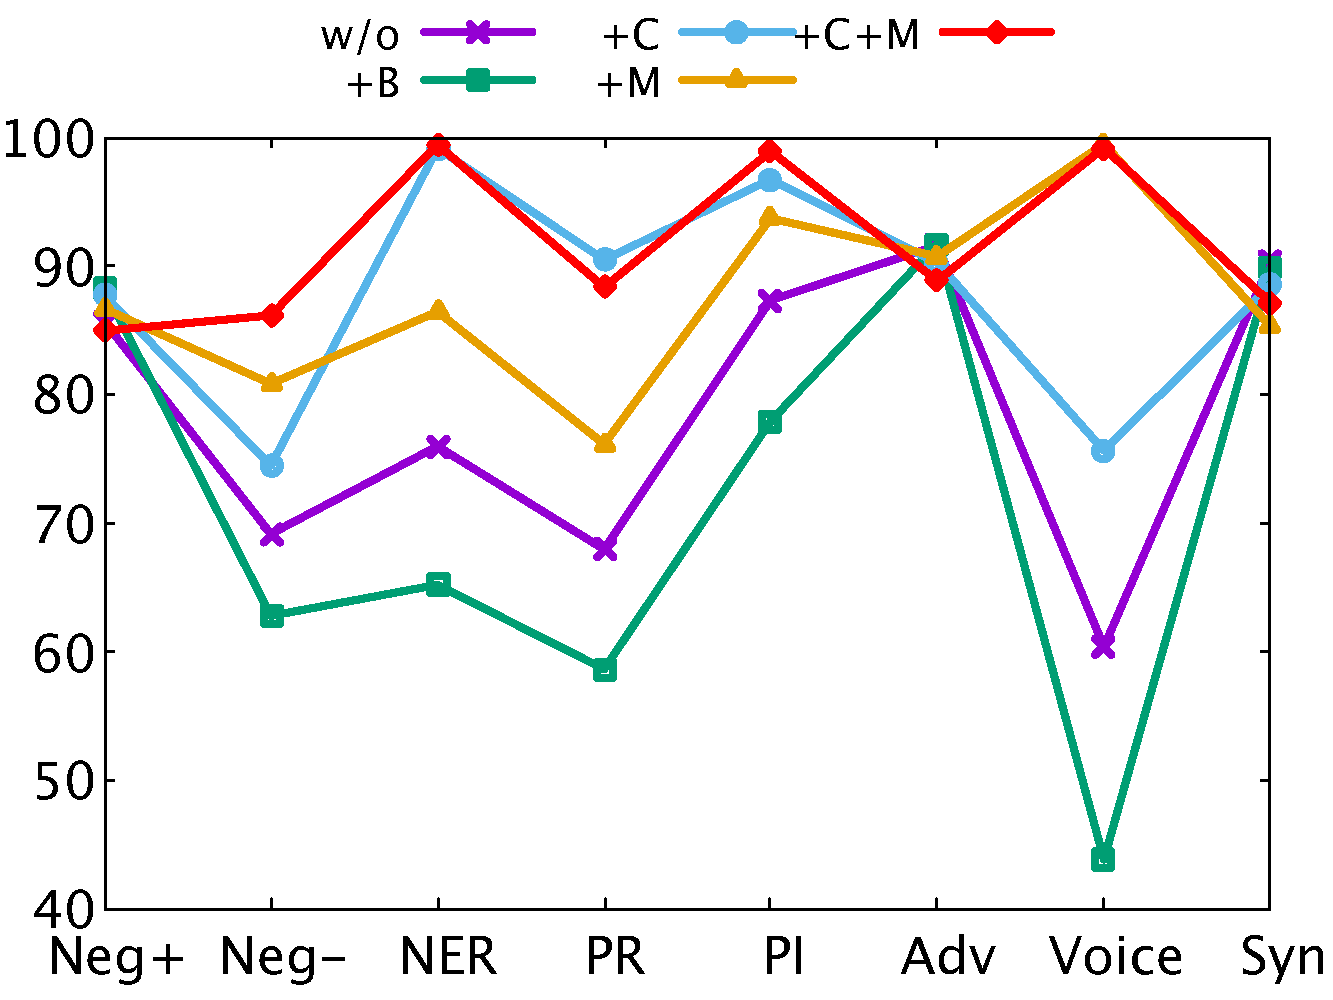
\includegraphics[width=0.6\columnwidth]{data/roc_roberta.pdf}
%   \caption{Detailed stress test with different aspects on ROC dataset. The x-axis indicates different stress test aspects and the y-axis indicates model accuracy in percentage.}
%   \label{fig:detailed}
% \end{figure}


%\begin{figure*}[!th]
%\centering
%\begin{subfigure}[b]{0.28\textwidth}
%\centering
%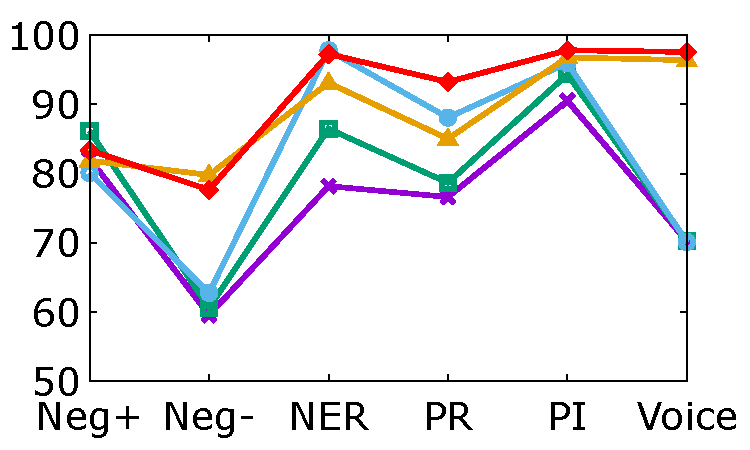
\includegraphics[width=\columnwidth]{data/roc_bert.pdf}
%\caption{BT (ROC)}
%\label{fig:roc_bert}
%\end{subfigure}
%\hfill
%\begin{subfigure}[b]{0.28\textwidth}
%\centering
%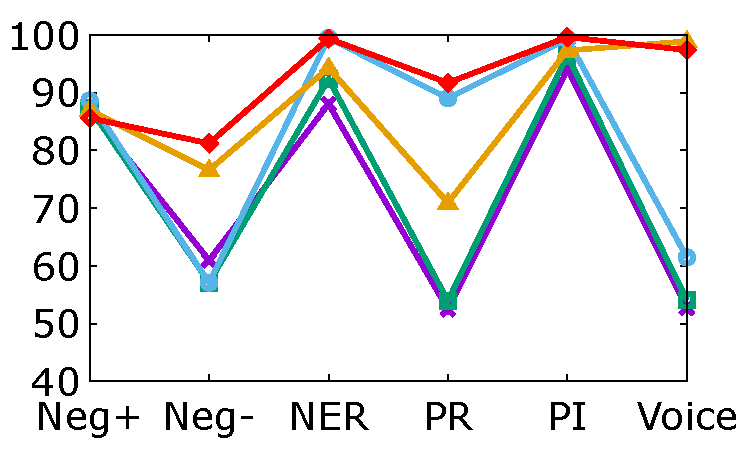
\includegraphics[width=\columnwidth]{data/roc_xlnet.pdf}
%\caption{XL (ROC)}
%\label{fig:roc_xlnet}
%\end{subfigure}
%\hfill
%\begin{subfigure}[b]{0.28\textwidth}
%\centering
%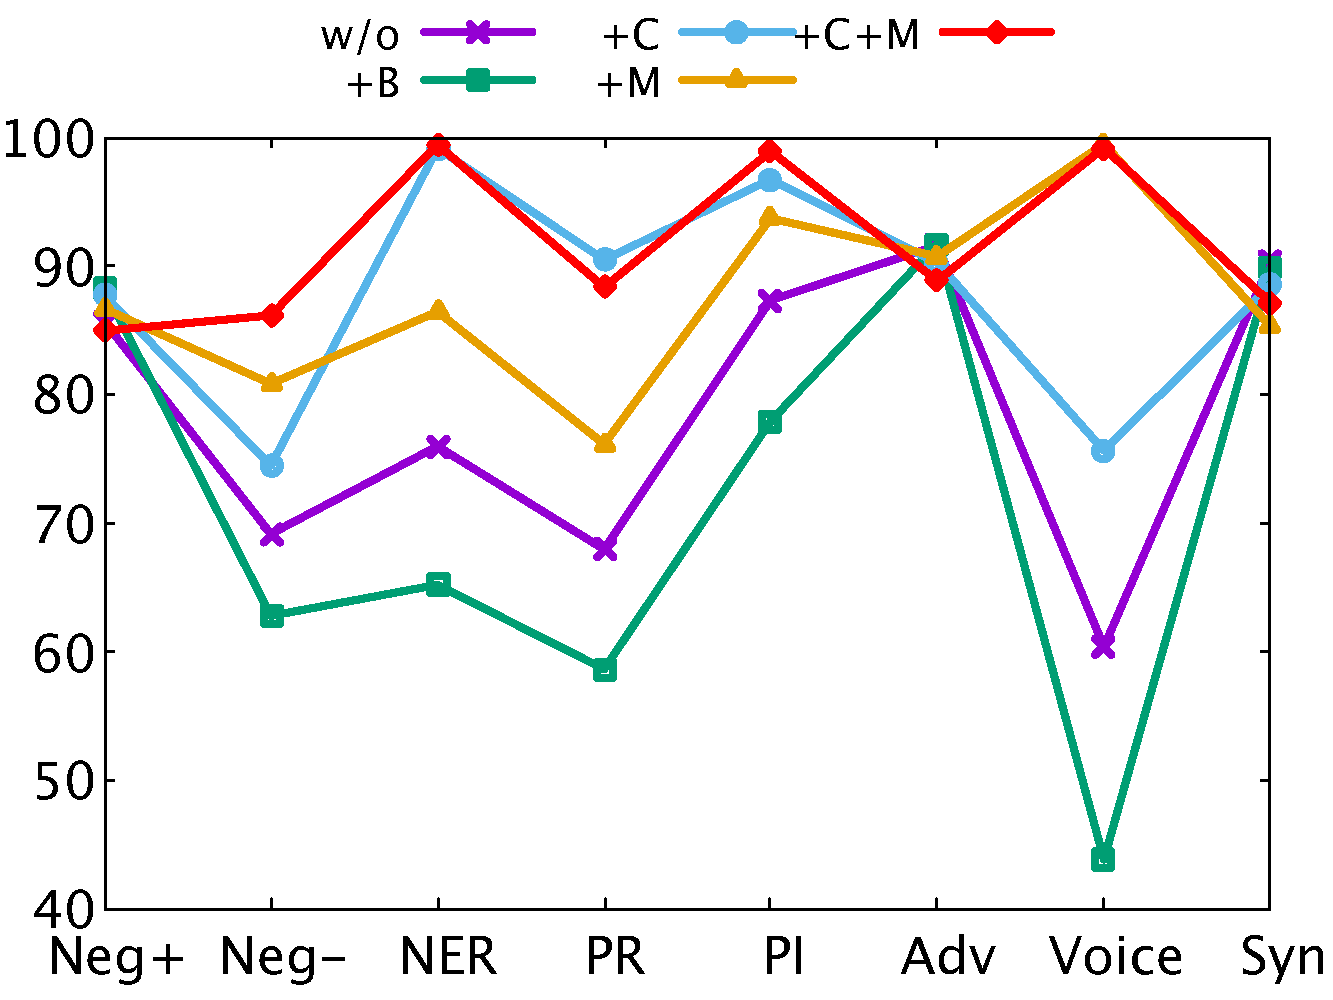
\includegraphics[width=\columnwidth]{data/roc_roberta.pdf}
%\caption{RB (ROC)}
%\label{fig:roc_roberta}
%\end{subfigure}
%\newpage
%\begin{subfigure}[b]{0.28\textwidth}
%\centering
%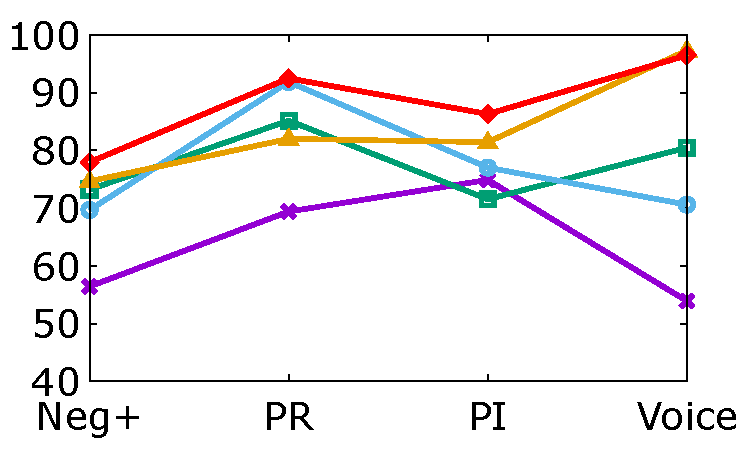
\includegraphics[width=\columnwidth]{data/copa_bert.pdf}
%\caption{BT (COPA)}
%\label{fig:copa_bert}
%\end{subfigure}
%\hfill
%\begin{subfigure}[b]{0.28\textwidth}
%\centering
%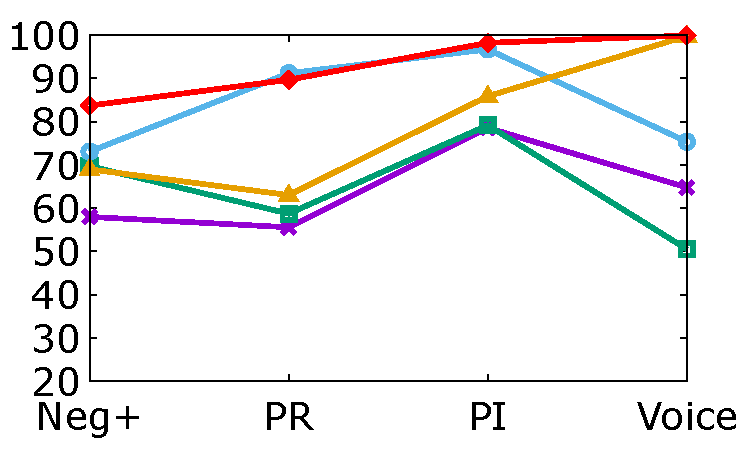
\includegraphics[width=\columnwidth]{data/copa_xlnet.pdf}
%\caption{XL (COPA)}
%\label{fig:copa_xlnet}
%\end{subfigure}
%\hfill
%\begin{subfigure}[b]{0.28\textwidth}
%\centering
%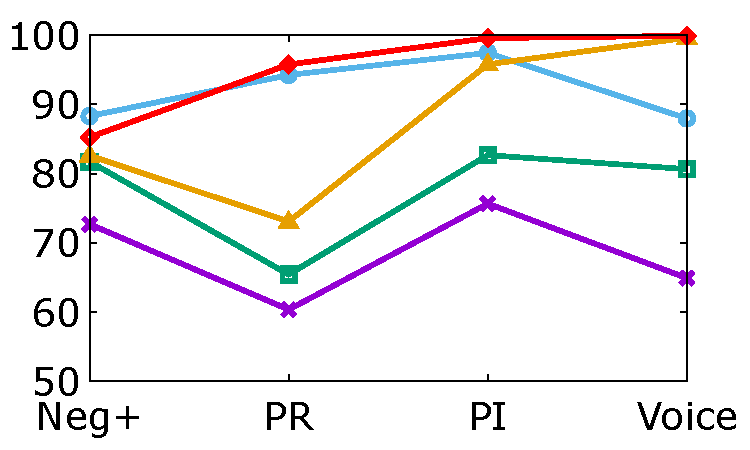
\includegraphics[width=\columnwidth]{data/copa_roberta.pdf}
%\caption{RB (COPA)}
%\label{fig:copa_roberta}
%\end{subfigure}
%\newpage
%\begin{subfigure}[b]{0.28\textwidth}
%\centering
%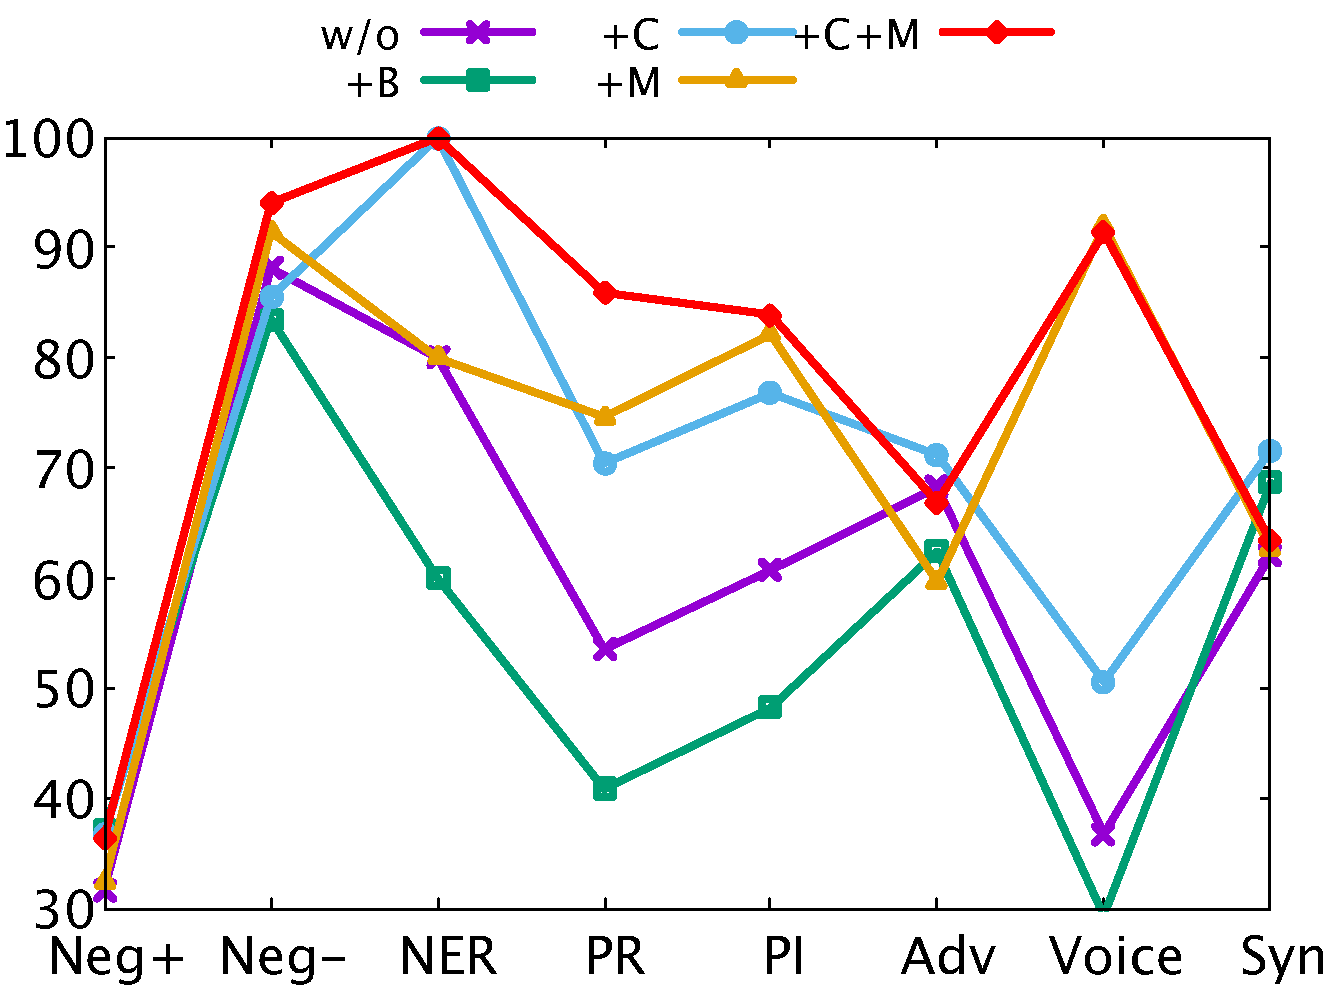
\includegraphics[width=\columnwidth]{data/arct_bert.pdf}
%\caption{BT (ARCT)}
%\label{fig:arct_bert}
%\end{subfigure}
%\hfill
%\begin{subfigure}[b]{0.28\textwidth}
%\centering
%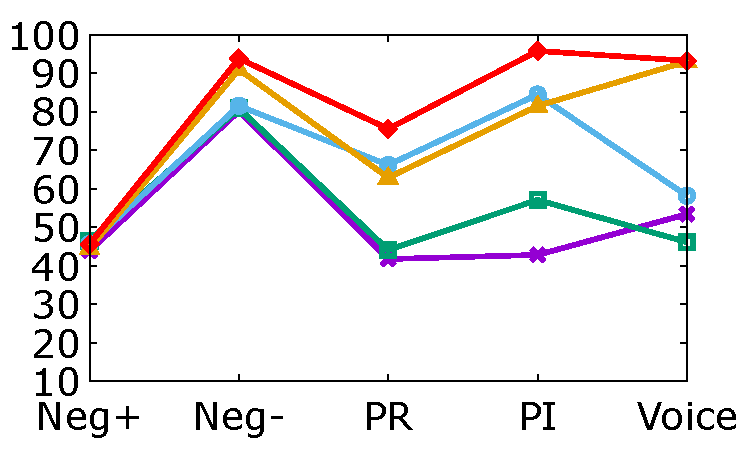
\includegraphics[width=\columnwidth]{data/arct_xlnet.pdf}
%\caption{XL (ARCT)}
%\label{fig:arct_xlnet}
%\end{subfigure}
%\hfill
%\begin{subfigure}[b]{0.28\textwidth}
%\centering
%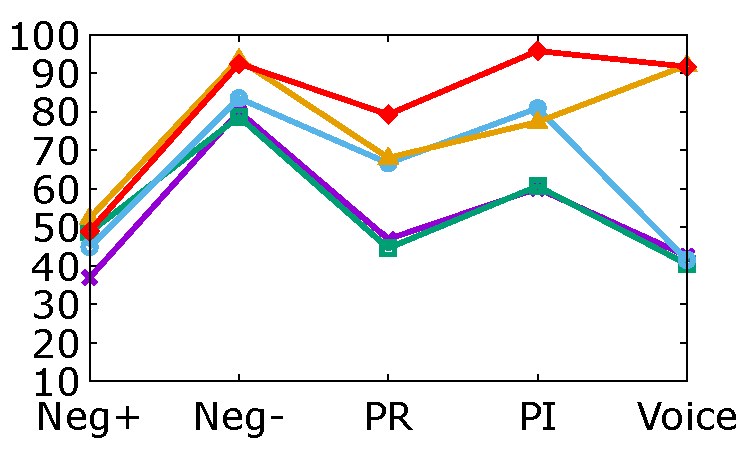
\includegraphics[width=\columnwidth]{data/arct_roberta.pdf}
%\caption{RB (ARCT)}
%\label{fig:arct_roberta}
%\end{subfigure}
%\newpage
%\begin{subfigure}[b]{0.28\textwidth}
%\centering
%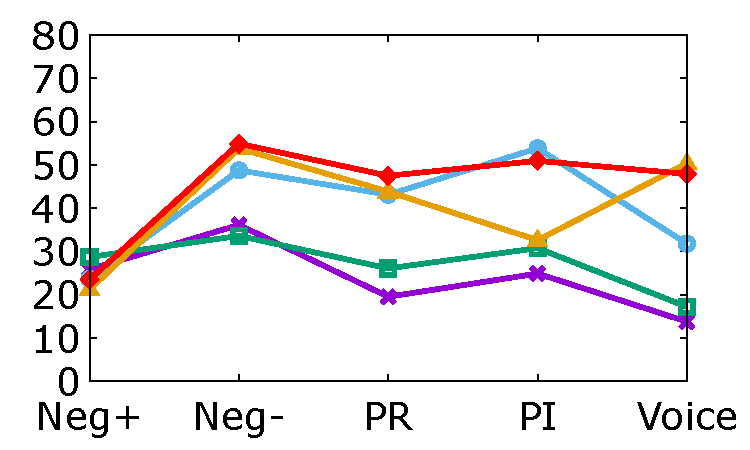
\includegraphics[width=\columnwidth]{data/reclor_bert.pdf}
%\caption{BT (RECLOR)}
%\label{fig:reclor_bert}
%\end{subfigure}
%\hfill
%\begin{subfigure}[b]{0.28\textwidth}
%\centering
%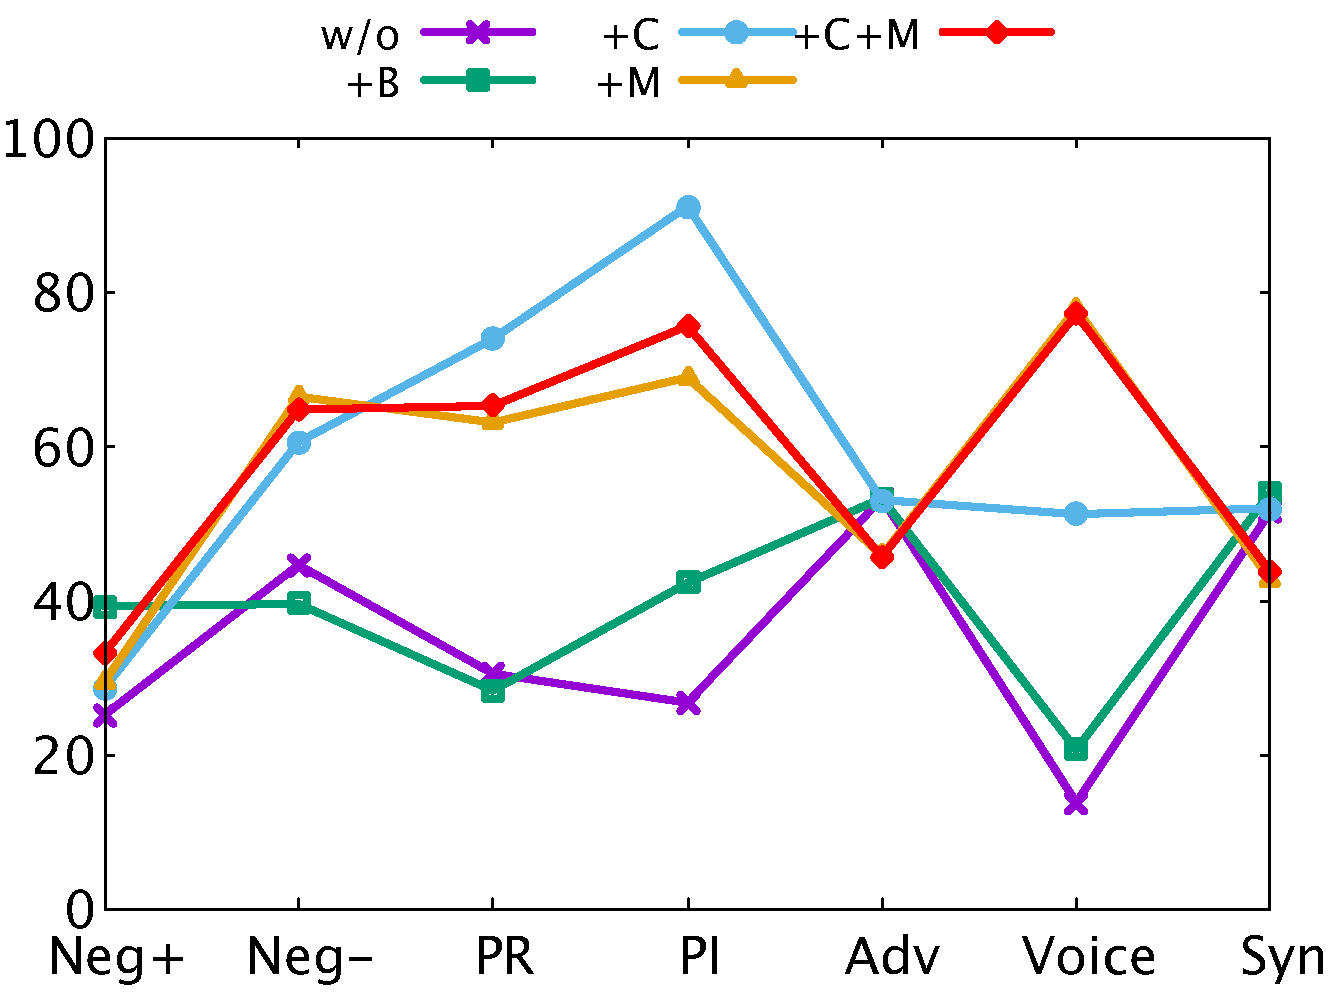
\includegraphics[width=\columnwidth]{data/reclor_xlnet.pdf}
%\caption{XL (RECLOR))}
%\label{fig:reclor_xlnet}
%\end{subfigure}
%\hfill
%\begin{subfigure}[b]{0.28\textwidth}
%\centering
%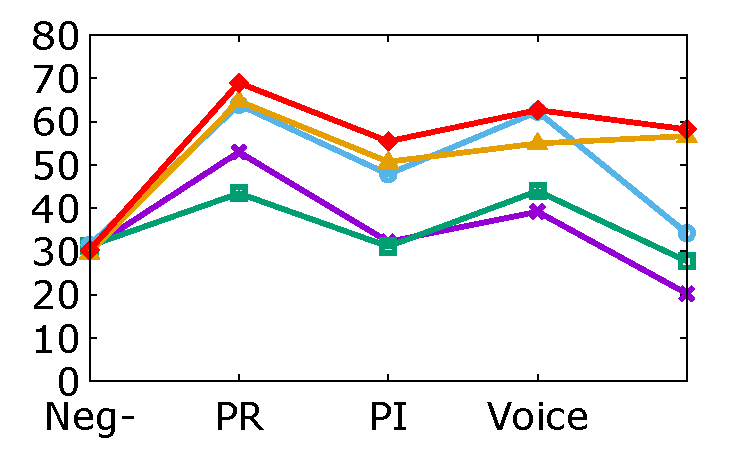
\includegraphics[width=\columnwidth]{data/reclor_roberta.pdf}
%\caption{RB (RECLOR)}
%\label{fig:arct_roberta}
%\end{subfigure}
%\newpage
%\begin{subfigure}[b]{1.0\textwidth}
%\centering
%
\includegraphics[width=0.4\columnwidth]{data/label.jpg}
%\label{fig:label}
%\end{subfigure}
%\caption{Fine-grained stress test with different aspects on 4 different tasks. 
%The x-axis in the figures indicates different stress test aspects and the y-axis indicates model accuracy in percentage.}
%%\KZ{Caption is wrong! most graphs are fine. 
%%But ReCLOR (RB) is a bit strange. 
%%Why is BT line exactly the same as the BT+C? And why is BT+B so bad?}}
%\label{fig:detail}
%\end{figure*}
%%
%
\begin{figure*}[!th]
\centering
\begin{subfigure}[b]{0.24\textwidth}
\centering
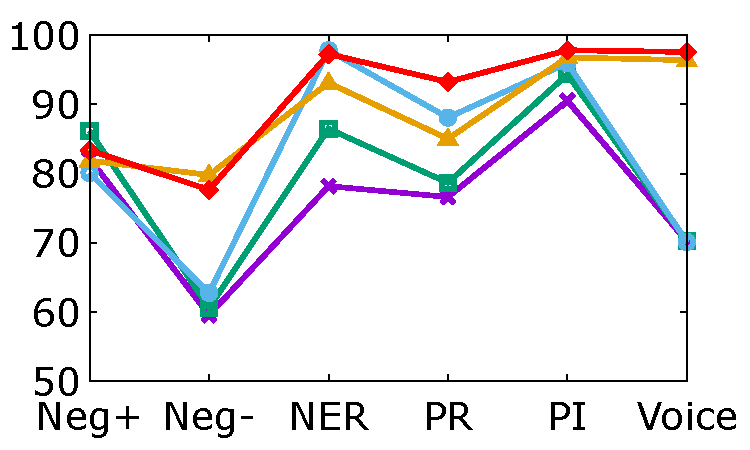
\includegraphics[width=\columnwidth]{data/roc_bert.pdf}
\caption{BT (ROC)}
\label{fig:roc_bert}
\end{subfigure}
\hfill
\begin{subfigure}[b]{0.24\textwidth}
\centering
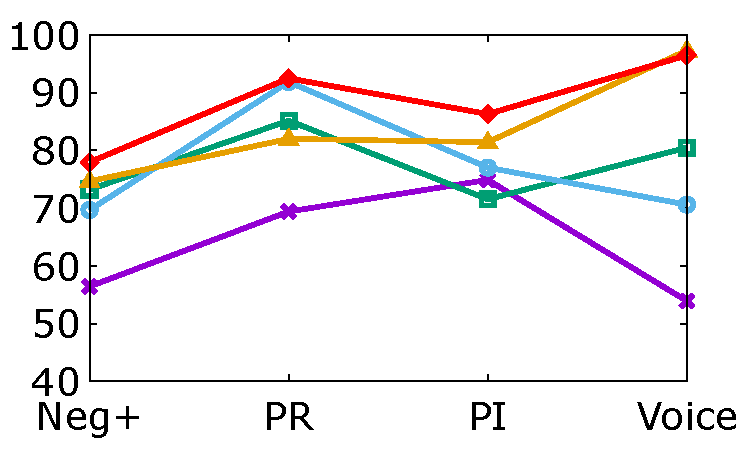
\includegraphics[width=\columnwidth]{data/copa_bert.pdf}
\caption{BT (COPA)}
\label{fig:copa_bert}
\end{subfigure}
\hfill
\begin{subfigure}[b]{0.24\textwidth}
\centering
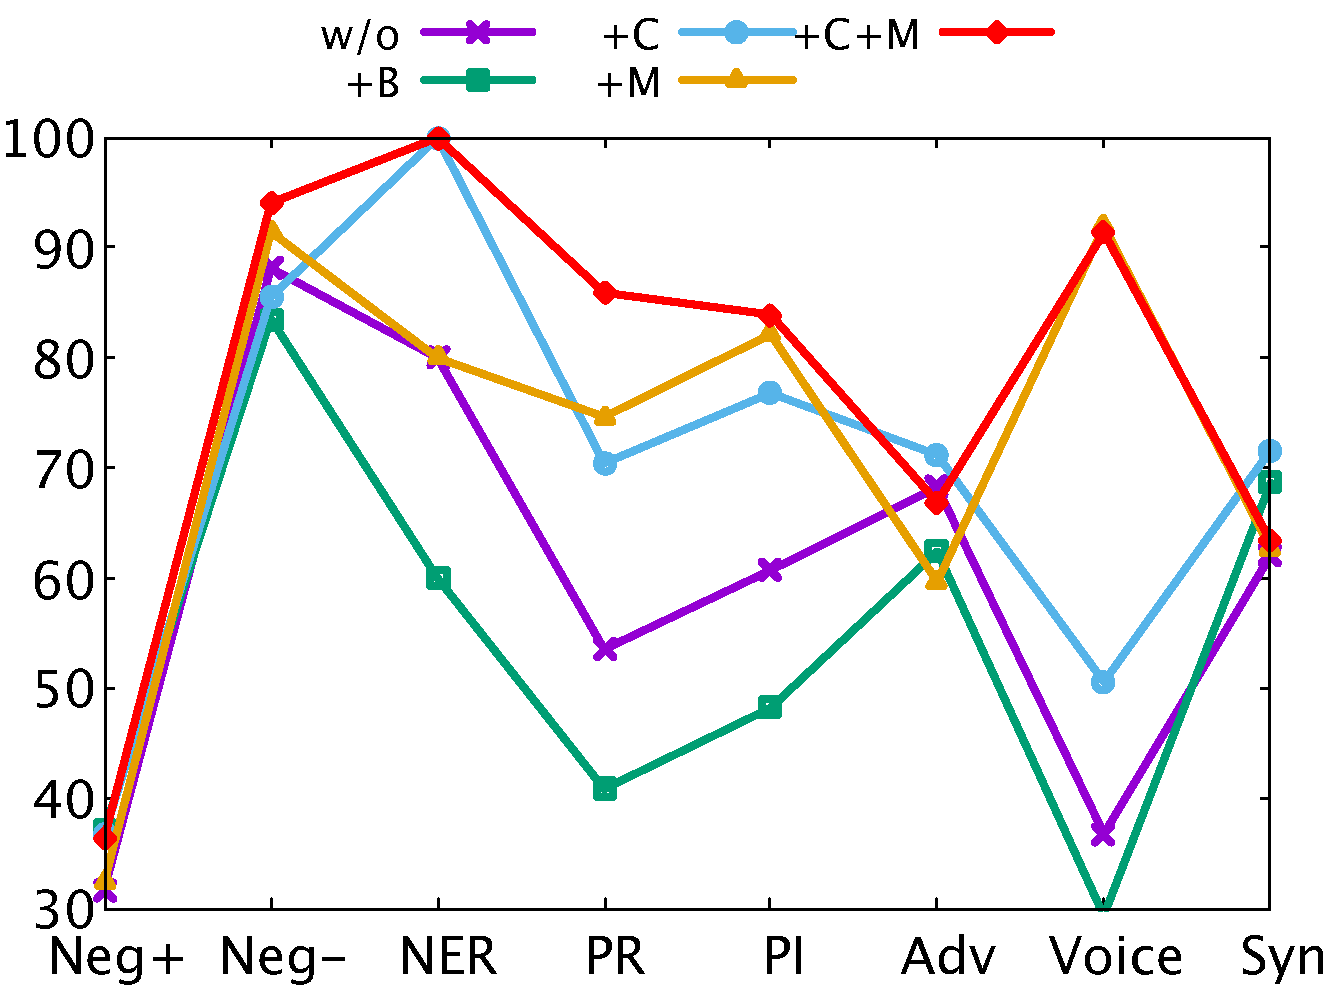
\includegraphics[width=\columnwidth]{data/arct_bert.pdf}
\caption{BT (ARCT)}
\label{fig:arct_bert}
\end{subfigure}
\hfill
\begin{subfigure}[b]{0.24\textwidth}
\centering
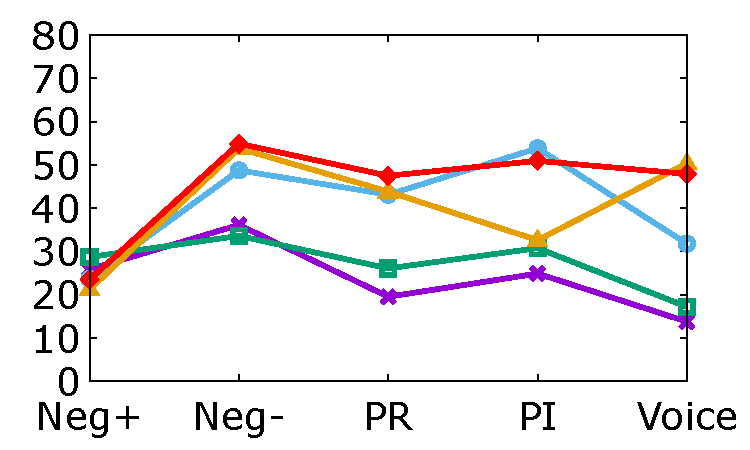
\includegraphics[width=\columnwidth]{data/reclor_bert.pdf}
\caption{BT (RECLOR)}
\label{fig:reclor_bert}
\end{subfigure}
\newpage
\begin{subfigure}[b]{0.24\textwidth}
\centering
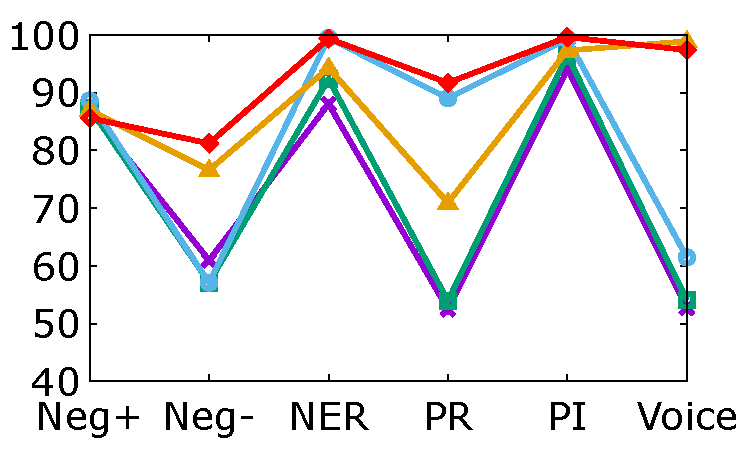
\includegraphics[width=\columnwidth]{data/roc_xlnet.pdf}
\caption{XL (ROC)}
\label{fig:roc_xlnet}
\end{subfigure}
\hfill
\begin{subfigure}[b]{0.24\textwidth}
\centering
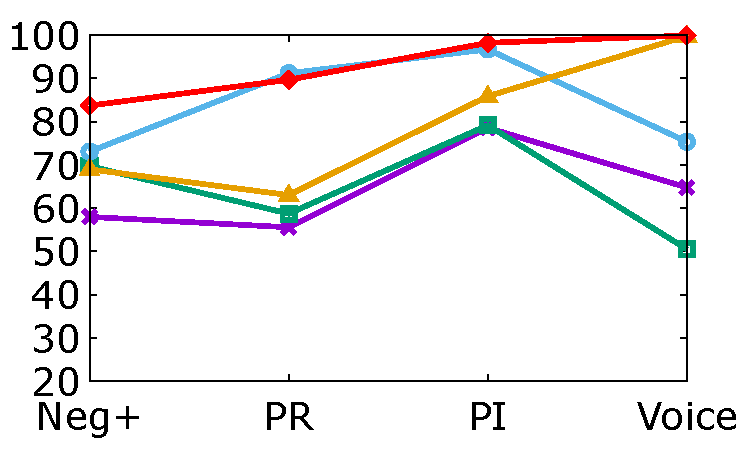
\includegraphics[width=\columnwidth]{data/copa_xlnet.pdf}
\caption{XL (COPA)}
\label{fig:copa_xlnet}
\end{subfigure}
\hfill
\begin{subfigure}[b]{0.24\textwidth}
\centering
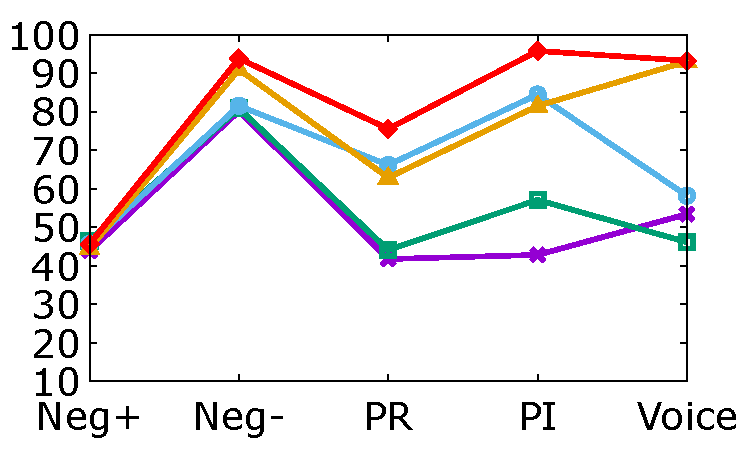
\includegraphics[width=\columnwidth]{data/arct_xlnet.pdf}
\caption{XL (ARCT)}
\label{fig:arct_xlnet}
\end{subfigure}
\hfill
\begin{subfigure}[b]{0.24\textwidth}
\centering
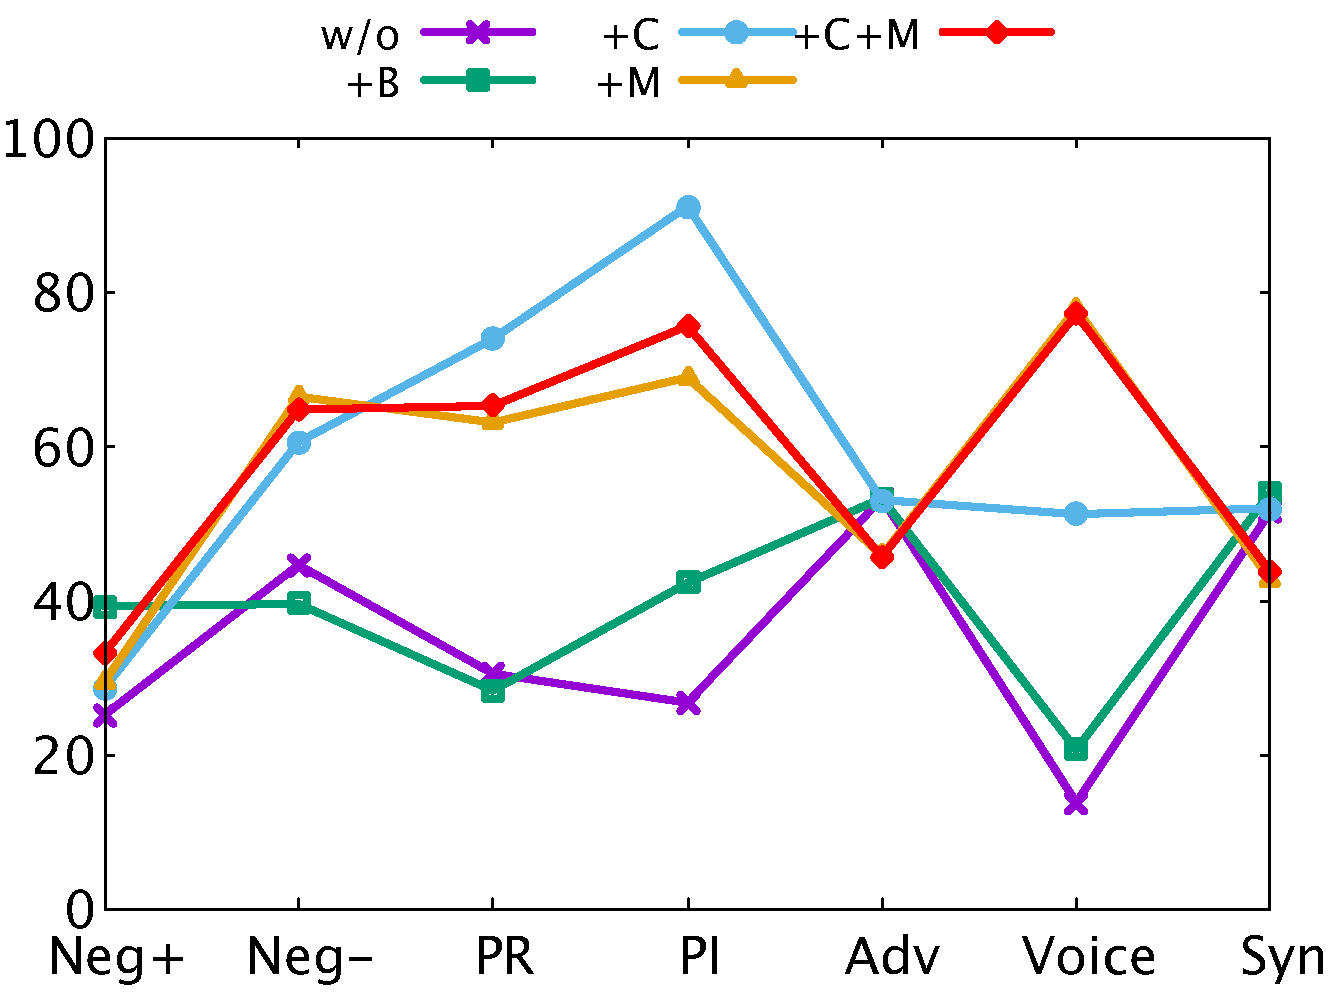
\includegraphics[width=\columnwidth]{data/reclor_xlnet.pdf}
\caption{XL (RECLOR))}
\label{fig:reclor_xlnet}
\end{subfigure}
\newpage
\begin{subfigure}[b]{0.24\textwidth}
\centering
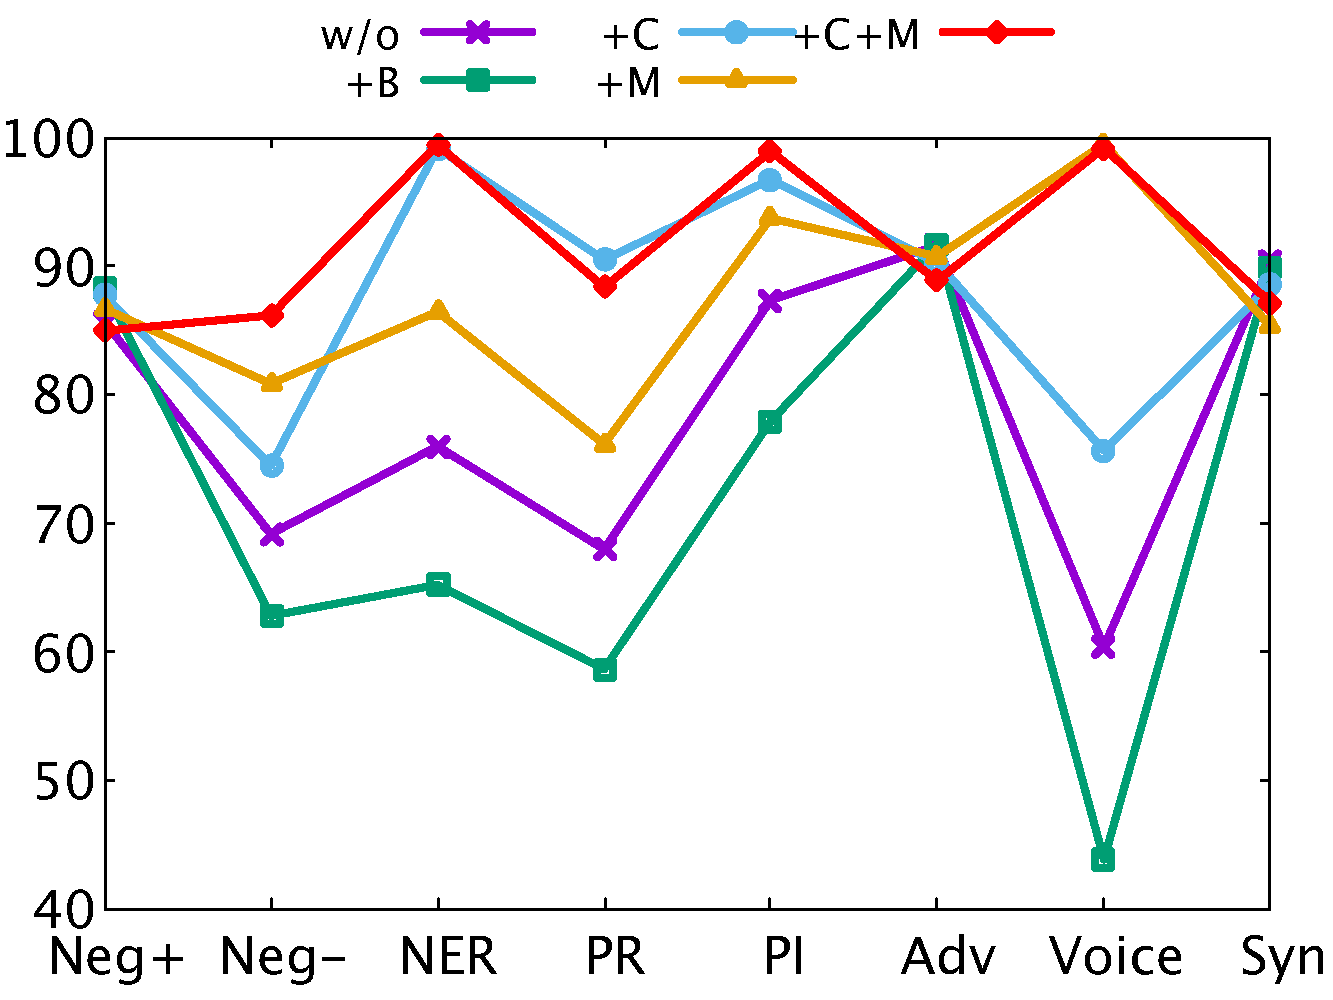
\includegraphics[width=\columnwidth]{data/roc_roberta.pdf}
\caption{RB (ROC)}
\label{fig:roc_roberta}
\end{subfigure}
\hfill
\begin{subfigure}[b]{0.24\textwidth}
\centering
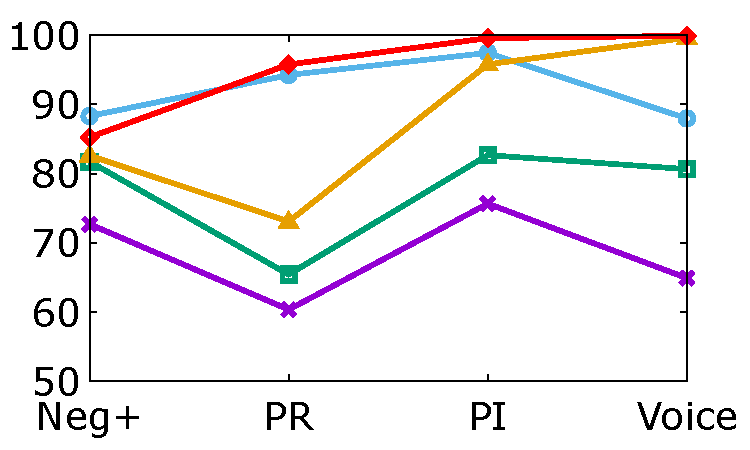
\includegraphics[width=\columnwidth]{data/copa_roberta.pdf}
\caption{RB (COPA)}
\label{fig:copa_roberta}
\end{subfigure}
\hfill
\begin{subfigure}[b]{0.24\textwidth}
\centering
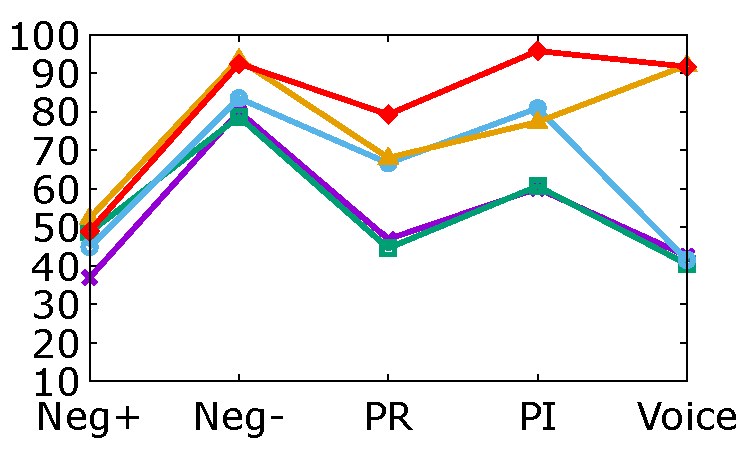
\includegraphics[width=\columnwidth]{data/arct_roberta.pdf}
\caption{RB (ARCT)}
\label{fig:arct_roberta}
\end{subfigure}
\hfill
\begin{subfigure}[b]{0.24\textwidth}
\centering
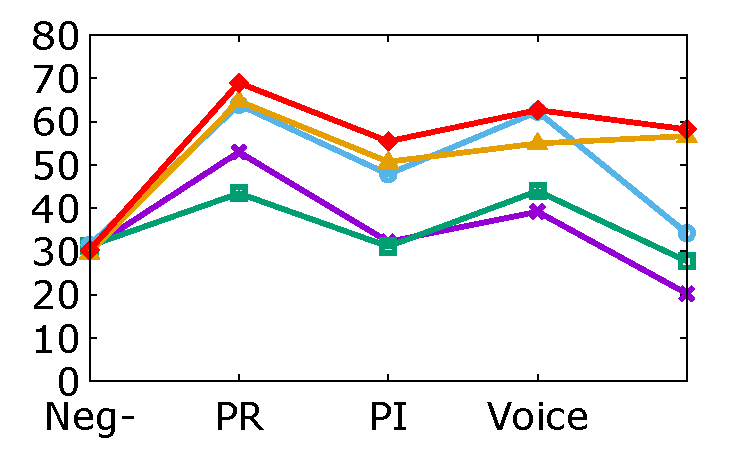
\includegraphics[width=\columnwidth]{data/reclor_roberta.pdf}
\caption{RB (RECLOR)}
\label{fig:arct_roberta}
\end{subfigure}
\newpage
\begin{subfigure}[b]{1.0\textwidth}
\centering
\includegraphics[width=0.4\columnwidth]{data/label.jpg}
\label{fig:label}
\end{subfigure}
\caption{Fine-grained stress test with different aspects on 4 different tasks. 
The x-axis in the figures indicates different stress test aspects and the y-axis indicates model accuracy in percentage.}
%\KZ{Caption is wrong! most graphs are fine. 
%But ReCLOR (RB) is a bit strange. 
%Why is BT line exactly the same as the BT+C? And why is BT+B so bad?}}
\label{fig:detail}
\end{figure*}
%
\subsubsection{Fine-grained results}
\label{sec:fine-grained}
We proceed to break down the results in \tabref{tab:stressresults} into accuracies on stress tests
created by different operators. 
%We show the detailed results in~\figref{fig:detail} 
%Concretely, six different aspects of stress test data are 
%utilized for testing.
COPA and RECLOR datasets do not show all six operators
because some of the operators generate too little data
for them, as shown in \tabref{tab:cases}. 
%The x-axis in the figures indicates different stress test aspects 
%and the y-axis indicates model accuracy in percentage.
%We apply the proposed two operators \textit{crossover} and \textit{mutation} to BERT, XLNet and RoBERTa 
%models and compare it with back-translation.
%and test on various stress test cases with different aspects. 
The corresponding results are presented in~\figref{fig:detail}. 
We observe that the vanilla model in purple and back-translation in green show
worse results across different aspects than other lines. 
The models trained with data augmented by \textit{crossover} and \textit{mutation} 
(the red lines) are generally more robust than others.
%\KZ{It is consistent with our overall results in~\tabref{tab:results}.} 
Please refer to Appendix A. 
%\footnote{There are some dashes in the table because the } 
for complete results. 
%\KZ{You need to explain why there are some dashes in the table in appendix.}

%We also observe that the 
%accuracy performance points for ``Syn'' and ``Adv'' are concentrated 
%but scattered on other operator aspects. 
Since every type of stress tests 
%(except ``Syn'' and ``Adv) 
can evaluate if a model is robust, particularly if it considers the 
premise by giving it two very similar choices, 
the above results on the stress tests of all types show that our two methods do 
%improves the model robustness, and may even encourage the models to look toward the
reduce short-circuits, and may even encourage the models to look toward the
premises.
We will provide additional pieces of evidence to confirm this in the next two subsections.

%\KZ{The weakness can be on the same table as the improvements
%to save space.}
%\KZ{Check the following analysis to make sure it's consistent with the tables.}

%Compared with 
%base models without data augmentation, we find that 
%all four data augmentation methods moderately improve
%the models when tested on the original test set. 
%In ROC, accuracy of BERT and RoBERTa trained with crossover augmented data 
%exceeds base models and ranks top. Crossover method also works on COPA. 
%Even though back-translation obtains higher score mostly on ARCT and RECLOR,
%crossover, mutation and crossover+mutation barely fall below the base model. 
%
%Augmentation fares much better in the ``Stress'' columns, though
%different methods show varying degree of success.
%Compared with the model without data augmentation, 
%the performance of models with crossover 
%has always been greatly improved (i.e., by 21.44\% for BERT on COPA).
%It indicates that reducing the short circuits 
%is a good way to improve the robustness of a model.
%The performance of new models with crossover has 
%great improvement for all models on different dataset 
%compared with the model without data augmentation, like 21.44% for BERT on COPA. 
%Mutation alone can also help with robustness on stress test better than crossover.
%This result suggests that mutation is a good method 
%for enhancing the robustness of models. 
%Though, mutation may be not a 
%good method to decrease the short circuits (\secref{sec:fix-sc}). 
%Overall, crossover+mutation 
%can mostly get the best performance on the stress test except for 
%training on RECLOR with RoBERTa. 
%to This result indicates that this kind of data can prevent models from being confused 
%by simple perturbations thus improving the robustness of models. 
%Besides, we can also find that back-translation doesn't improve the models' robustness much.
%Crossover alone can also help with robustness on stress test but 
%no better than mutation and crossover+mutation.  

%some of Table 5's AW scores being 
%some of Table 5's AW scores being 
%lower than AW for model w/o augmentation (e.g., 45.13 in (b)), 
%then the reason is AW is only a proxy test
%that catches majority of short circuit cases in our opinion, 
%but it's not perfect, as we pointed out in A2 of R1. 
%If you are referring to some accuracies in the Original columns 
%being lower than models w/o augmentation in Table 5 (e.g., 72.6 in (b)), 
%the reason is some models w/o augmentation might have 
%"cheated" to get high accuracy. Augmenting (C or M) corrects the
%biases in these models and may reduce the accuracy on the original test set.
%Nevertheless, all models after augmentation do better on the stress tests.

%have least short circuits based on BERT and XLNet. 
%Crossover+mutation based on RoBERTa takes less short circuits than others. 
%In the CO and AW columns, the result are consistent on ROC. 

%\subsection{White-box Attention Weights~(AW)}
%\KZ{Here we first talk about human testing by visualizastion,
%then talk about how to automatic it thru code.}

%show human annotation results of bert, roberta, xlnet.
%For exploiting whether attention-based models are suffered from short circuits, 
%we propose to 
%use the AW method which we have described in~\secref{}.
%It is noted that t\_1 is greater than t\_2. 
%Here t\_1 and t\_2 are tuned to 0.14 and 0.13 separately.

\subsection{Choice-only Test}
\label{sec:choice-only}

%In this section, we use choice-only test for different models on four tasks. 
%We have shown the effectiveness of \textit{crossover} and \textit{mutation} on in robustness test. 
The end-to-end test has shown the success of our data augmentation 
methods. To further explore the reason behind the performance gain, 
we also use choice-only test here.

%somewhat confirm the reason for model improvement with data augmentation 
%strategies. Moreover, this test is used to further explore 
%whether our strategies can encourage models pay more attention to premise.
In choice-only test, we only feed choices into a model without a premise which is replaced 
by an empty string. This way, 
models cannot utilize the relationship between premise and choices. 
%what we can know whether a model can 
%solve cases easily without awaring premise by test accuracy. 
Normally, we would expect the model to make arbitrary choices.
However, if a model can easily ``guess'' the ``right'' choice which 
normally requires the relationship between premise and choices,  
one possibility is that this model cheats on evaluation procedure and 
may be fragile. Thus, the higher score may indicate more use of short-circuits.

In~\figref{fig:choice-only}, we observe that in choice-only tests,
the accuracy of models augmented with \textit{crossover} and \textit{mutation} 
(red line) drops the most. 
Sometimes the performances are similar to random selection, e.g., 
RB+C+M on ARCT (56.38\%), which indicates that models 
are no longer cheating. 
In other words, models augmented by crossover and mutation 
are more likely to consider the premises. 
The results on the choice-only tests provide another perspective for us
to re-assure that models augmented with crossover and mutation can reduce
short circuits and thus model fragility.

%\KZ{Rephrase: 
%However, another possibility reason for lower choice-only test accuracy 
%that is also not ruled out is that 
%even if the model can tell the result with only choices, 
%it still chooses to look at the premise context. 
%Although high scores do not necessarily imply models 
%are not looking forward, low scores necessarily mean that models cannot 
%conclude that solely relying on choices.} 

%\begin{table}[th]
%\centering
%\scriptsize
%\begin{tabular}{c|rrrr}
%\toprule
%\textbf{Model} & \textbf{ROC} & \textbf{COPA} & \textbf{ARCT} & \textbf{RECLOR} \\ \midrule
%%BT  &98.76 &89.68&\textbf{99.65}&82.46    \\ \hline
%%BT+B  &99.26 &96.79   &99.34  &86.01  \\ \hline
%%BT+C  &\textbf{99.69} &\textbf{98.35}&98.37   &80 \\ \hline
%%BT+M  &99.26 & 95.17 &98.67 &82.48    \\ \hline
%%BT+C+M  &98.82 &96.96 &98.00 &\textbf{96.79}  \\ \midrule
%%XL  &28.08 &93.16 & 85.67 & 79.64 \\ \hline
%%XL+B  &19.27  &91.46 &95.73 & 81.40   \\ \hline
%%XL+C  &\textbf{64.58} &45.13  &55.59  &\textbf{87.87} \\ \hline
%%XL+M  &62.77  &96.85 & \textbf{95.74}& 72.76  \\ \hline
%%XL+C+M  &60.25 & \textbf{98.51}&86.26 &   48.71\\ \midrule
%%RB  &77.41 & 80.89 & 99.14& 85.88 \\ \hline
%%RB+B  &   58.15 &\textbf{96.36}   & 97.78& 15.69  \\ \hline
%%RB+C  &   82.71& 89.62&79.19& 89.68\\ \hline
%%RB+M  &71.73& 62.26& \textbf{100.00}&\textbf{100.00}  \\ \hline
%%RB+C+M  &\textbf{93.31} &61.89    &71.47 & 89.26\\ 
%%
%BT (w/o)&54.62&51.4&61.94&42.8 \\ \hline
%BT+B&58.26&50.8&64.41&39.2  \\ \hline
%BT+C&51.2&48.2&55.63&30.8  \\ \hline
%BT+M&51.79&48.8&55.18&38   \\ \hline
%BT+C+M&43.56&49.4&52.03&33.8  \\ \midrule
%XL (w/o)&71.14&57&65.99&42.2 \\ \hline
%XL+B&73.17&60&66.89&41.4  \\ \hline
%XL+C&65.63&55&55.86&34.2  \\ \hline
%XL+M&71.94&57.8&66.22&42  \\ \hline
%XL+C+M&66.22&58.4&62.84&35  \\ \midrule
%RB (w/o)&73.97&59.4&67.79&30.2 \\ \hline
%RB+B&74.77&61.4&69.37&42.2  \\ \hline
%RB+C&73.06&58.4&68.47&34.6  \\ \hline
%RB+M&70.34&56&61.49&40      \\ \hline
%RB+C+M&71.3&54.8&67.79&32.2  \\ 
%\bottomrule
%\end{tabular}
%\caption{Choice-only test for transformer-based models on 4 datasets. All numbers are percentages (\%)}
%%\KZ{I assume this is the ending-only test? But isn't scriptsizeer the better
%%for ending-only tests?}}
%\label{tab:only-test}
%\end{table}
%
\begin{figure}[th]
    \centering
    \includegraphics[width=0.7\columnwidth]{data/choice-only.pdf}
    \caption{Choice-only test: Accuracies of different data augmentation methods with 3 models on 4 tasks. 
    The detailed numbers are in Appendix B.}
    \label{fig:choice-only}
\end{figure}

However, one may argue that even if a model can 
choose or ``guess'' correctly given only the choices but no premise, 
it may still have the ability to look at the premise if it's given one,
like in the end-to-end test.
Therefore, next we conduct an additional case study to show that short-circuit
does take place and our augmentation methods alleviate it.

\subsection{Case Study}
\label{sec:case}

%\begin{figure}[th!]
%\centering
%\begin{subfigure}[b]{0.21\textwidth}
%\centering
%
%\framebox{\includegraphics[width=\columnwidth]{figure/case_original.eps}}
%\caption{RB(w/o)}
%\label{fig:case_original}
%\end{subfigure}
%\hfill
%\begin{subfigure}[b]{0.21\textwidth}
%\centering
%\framebox{\includegraphics[width=\columnwidth]{figure/case_b.eps}}
%\caption{RB+B}
%\label{fig:case_b}
%\end{subfigure}
%\hfill
%\newpage
%\begin{subfigure}[b]{0.21\textwidth}
%\centering
%\framebox{\includegraphics[width=\columnwidth]{figure/case_c.eps}}
%\caption{RB+C}
%\label{fig:case_c}
%\end{subfigure}
%\hfill
%\begin{subfigure}[b]{0.21\textwidth}
%\centering
%\framebox{\includegraphics[width=\columnwidth]{figure/case_cm.eps}}
%\caption{RB+C+M}
%\label{fig:case_cm}
%\end{subfigure}
%\caption{Attention map on a COPA example for models.}
%%\KZ{Caption is wrong! most graphs are fine. 
%%But ReCLOR (RB) is a bit strange. 
%%Why is BT line exactly the same as the BT+C? And why is BT+B so bad?}}
%\label{fig:case}
%\end{figure}
%

%In \figref{fig:case}, 
%%illustration. There is no positive attention value in front of the 
%%fourth sentence, so we intercept it from where it is worth. 
%RoBERTa trained on the original training set fails to pick up the 
%relation between ``pushed'' and ``opened''. 
%%right choice likely due to there being virtually no attention 
%%connection between words in the choice and words in the premise. 
%After training with \textit{crossover} data augmentation, 
%the model learns to build contextual reasoning  
%by attending to relevant concepts in the premise. 
%%i.e., ``show'' in this example. The rationale behind 
%%such a change of attention pattern is that, 
%%in a MCQ created by crossover operation, 
%%the model needs to combine information 
%%in the premise to effectively 
%%distinguish the true ``right'' choice from the wrong one, 
%%which is also a right choice in another MCQ. 
%to have not enhanced such abilities. We provide additional cases in Appendix C.

%\begin{figure}[th]
%\centering
%{\setlength{\fboxsep}{0pt}
%5\framebox{%
%\includegraphics[width=0.47\columnwidth]{figure/o_un.eps}
%}
%\hfill
%\framebox{%
%\includegraphics[width=0.47\columnwidth]{figure/cross_un.eps}
%}
%}
%\caption{Attention maps showing that RoBERTa short-circuits on a ROC
%question (left) and no longer short-circuits after data augmentation (right). \KZ{I suggest we show a few more cases here to be more convincing. Show the before and after. Before there's no attention to the
%premise, after there is.}}
%\label{fig:case_study}
%\end{figure}

%\begin{example}\label{ex:roc}
%An MCQ from ROC:\\ \\
%\noindent
%\textbf{Premise:} Sarah was home alone. She wanted to stay busy. She turned on the TV. 
%She found a reality show to watch.  \\
%\textbf{Choice 1:} Sarah then happily watched the show.  \checksymbol  \\
%\textbf{Choice 2:} Sarah could not find anything to watch. \crosssymbol
%\end{example}

Our case study is a series of white-box tests that demonstrate
the change in attention patterns.

We take an example from ROC which is shown in~\tabref{table:dataset}.
We explore BERT-based models by 
analyzing their attention maps on this case in~\figref{fig:roc_bert}.  
In this example, the word ``show'' in the premise is strongly
related to the token ``reality show'' in the right choice from human knowledge. 
%The relationship between these two words is the key to answering this question. 
%We explore different models with the augmentation method with attention map 
%to visualize if these two words have a relationship or not.
The attention map is visualized via an off-the-shelf tool~\cite{vig-2019-multiscale}.


There is no positive attention value in front of the fourth sentence, 
so we intercept it from where it is worth. 
BERT trained on the original training set fails 
to pick up the right choice likely due to there being 
virtually no attention connection between words in 
the choice and words in the premise.
After training with \textit{crossover} data augmentation, 
the model learns  
to pay attention to the premise and the relationship 
between premise and choices. 
i.e., ``show'' in this example. 
Similar trends also exist for the \textit{mutation} operation in \figref{fig:roc_m} 
and the combination of \textit{crossover} 
and \textit{mutation} operation in~\figref{fig:roc_cm}. 
The rationale behind 
such a change of attention pattern is that, 
in an MCQ created by \textit{crossover} operation (\figref{fig:roc_c}), \textit{mutation}(\figref{fig:roc_m}), 
and the combination of them (\figref{fig:roc_cm}), 
the model needs to combine the information 
in the premise to effectively 
distinguish the true ``right'' choice from the wrong one. 
However, the light and sparse attention color blocks on the attention map for back-translation 
in \figref{fig:roc_b} indicate back-translation 
can not help BERT connect the choice and premise very well in this question.
These observations empirically demonstrate the effectiveness of our methods 
in encouraging the model to pay attention to the premise to reduce 
short circuits. We provide additional cases in Appendix C. 

%\begin{figure}[th!]
%\centering
%\begin{subfigure}[b]{0.35\textwidth}
%\centering
%\framebox{\includegraphics[width=\columnwidth]{figure/roc_b.eps}}
%\caption{BT+B}
%\label{fig:roc_b}
%\end{subfigure}
%\hfill
%\begin{subfigure}[b]{0.35\textwidth}
%\centering
%\framebox{\includegraphics[width=\columnwidth]{figure/roc_c.eps}}
%\caption{BT+C}
%\label{fig:roc_c}
%\end{subfigure}
%%\hfill
%\newpage
%\begin{subfigure}[b]{0.35\textwidth}
%\centering
%\framebox{\includegraphics[width=\columnwidth]{figure/roc_m.eps}}
%\caption{BT+M}
%\label{fig:roc_m}
%\end{subfigure}
%\hfill
%\begin{subfigure}[b]{0.35\textwidth}
%\centering
%\framebox{\includegraphics[width=\columnwidth]{figure/roc_cm.eps}}
%\caption{BT+C+M}
%\label{fig:roc_cm}
%\end{subfigure}
%\caption{Attention map on a ROC example for BERT-based models.}
%%\KZ{Caption is wrong! most graphs are fine. 
%%But ReCLOR (RB) is a bit strange. 
%%Why is BT line exactly the same as the BT+C? And why is BT+B so bad?}}
%\label{fig:roc_bert}
%\end{figure}
%
\begin{figure}[h!]
\centering
\begin{minipage}{0.30\linewidth}
    \centering
    \fbox{\includegraphics[width=\linewidth]{figure/roc_b.eps}}
    \caption*{BT+B}
    \label{fig:roc_b}
\end{minipage}
\hspace{0.5cm}
\begin{minipage}{0.30\linewidth}
    \centering
    \fbox{\includegraphics[width=\linewidth]{figure/roc_c.eps}}
    \caption*{BT+C}
    \label{fig:roc_c}
\end{minipage}
\hspace{1.5cm}
\vspace{0.5cm}
\begin{minipage}{0.30\linewidth}
    \centering
    \fbox{\includegraphics[width=\linewidth]{figure/roc_m.eps}}
    \caption*{BT+M}
    \label{fig:roc_m}
\end{minipage}
\hspace{0.5cm}
\begin{minipage}{0.30\linewidth}
    \centering
    \fbox{\includegraphics[width=\linewidth]{figure/roc_cm.eps}}
    \caption*{BT+C+M}
    \label{fig:roc_cm}
\end{minipage}
\caption{Attention map on a ROC example for BERT-based models.}
\label{fig:roc_bert}
\end{figure}


%\subsection{Discussion}
%
%From previous test results on original test, stress test, choice-only test and test cases analysis, 
%we can illustrate that \textit{crossover} and \textit{mutation} can teach models to pay more attention to 
%the relationship between the premise and the choices. However, there is a doubt that \textit{mutation} 
%can triger a new bias cue that once the model find the choice is ingrammatically, it will choose another 
%choice. 
%%Thus we make another experiment to verify whether the augmentation operator \textit{mutation} can 
%Thus in this section, we make an experiment that we generate new grammar test cases which only 
%mutate words in the right choices. If models' prediction results are unchanged, 
%it can indicate that these models which trained with augmentation 
%data can't be easily triggered by the grammatical cues. The test result for models are shown in \tabref{tab:mutate} on ROC dataset. 
%We can find that the predicting change rate for +M models are not higher than vanilla models which illustrates 
%that +M will not introduce extra grammatical bias cues.
%\begin{table}[th!]
%   \centering
%   \scriptsize
%   \begin{tabular}{lc}
%       \toprule
%       \textbf{Model}& Change Rate \\
%       \midrule
%       BT(w/o)& 7.35\\
%       BT+M&6.37\\
%       \midrule
%       XL(w/o)&8.17 \\
%       XL+M&8.45 \\
%       \midrule
%       RB(w/o)&5.94\\
%       RB+M&5.73\\
%       \bottomrule
%   \end{tabular}
%   \caption{Grammatical sensitivity test on ROC dataset. All the numbers are percentage(\%)}
%   \label{tab:mutate}
%\end{table}



\section{Discussion and Future Work}
\label{sec:discussion}
In the era of large-scale language models, such as GPT-4~\cite{openai2023gpt4}, 
our work on addressing short circuits and enhancing 
data augmentation techniques is significant for 
improving the development and assessment of these models. 
By focusing on robustness, generalization, and interpretability, 
we contribute to more reliable and versatile systems 
that can handle a wide range of language reasoning tasks. 
Our work serves as a stepping stone for continued progress in the field, 
ensuring that models can effectively cope with diverse language challenges.

Future research directions include exploring alternative 
data augmentation techniques, incorporating explainability and 
interpretability methods, and developing new evaluation metrics and benchmarks. 
%Investigating model-agnostic data augmentation 
%approaches could also extend the applicability 
%of our findings to other language tasks and models, 
%further fostering improvements in natural language processing and advancing the robustness, generalization, and interpretability of large-scale language models in various natural language reasoning tasks 
for large-scale language models.

% !TEX root = ../main.tex

\section{Related Work}
%In this section, we review related works covering three aspects, namely using LLMs on mental health, general benchmarks and specific mental health benchmarks.
\paragraph*{LLMs on Mental Health}
Currently, there is relatively limited research utilizing LLMs in the field of mental health. Some studies have delved into the capabilities of LLMs for sentiment analysis and emotion reasoning ~\cite{kocon2023chatgpt, qin2023chatgpt, zhong2023can}. Lamichhane~\cite{Lamichhane2023chatgptapp}, Amin et al. ~\cite{amin2023will}, and Yang et al.~\cite{yang2023evaluations} conducted assessments of ChatGPT's performance across various classification tasks, including stress, depression, and suicide detection. The findings indicate that ChatGPT demonstrates initial potential for mental health applications, yet there remains significant room for improvement.

\paragraph*{General Benchmarks for LLMs}
To evaluate the performance of LLMs across different tasks, several benchmarks have been proposed. C-EVAL~\cite{huang2023ceval} assesses the advanced knowledge and reasoning capabilities of foundation models in Chinese. AGI-Eval~\cite{zhong2023agieval} serves as an evaluation framework for assessing the performance of foundation models in human-centric standardized exams. MMLU~\cite{hendrycks2021measuring} aims to develop a comprehensive test for evaluating text models in multi-task contexts. Big-Bench~\cite{srivastava2023beyond} introduces 204 challenging tasks covering various domains, aiming to evaluate tasks beyond the capabilities of existing language models. HELM ~\cite{helm2023liang} offers a comprehensive assessment, evaluating LLMs across various aspects, such as language understanding and common-sense reasoning. 
These benchmarks, while diverse and comprehensive, primarily emphasize general capabilities and do not cater specifically to the intricacies of mental health.

\paragraph*{Mental Health Benchmarks for LLMs}
Apart from general tasks, specific benchmarks are designed for certain downstream tasks. MultiMedQA~\cite{singhal2023large} focuses on medical question-answering, evaluating LLMs in terms of clinical knowledge and QA abilities. Mental-LLM~\cite{xu2023leveraging} focuses on evaluating the ability of LLMs to predict mental health outcomes through the analysis of online text data. Dialogue safety~\cite{qiu2023benchmark} focuses on the understanding of the safety of responses generated by LLMs in the context of mental health support. Compared to these benchmarks, PsyEval (1) provides a more targeted and comprehensive evaluation of LLMs' capabilities in addressing the unique challenges and nuances of mental health-related tasks. (2) fully considers the differences between the field of mental health and other disciplines.
However, these benchmarks, while addressing specific aspects of mental health or related fields, do not fully encompass the multifaceted nature of mental health issues.

%Contrastingly, our proposed PsyEval benchmark distinguishes itself by offering a more targeted and comprehensive evaluation, specifically designed for mental health-related tasks. PsyEval goes beyond assessing basic understanding or response safety, delving into the complexities unique to mental health. It recognizes that symptoms of mental disorders are subtle, subjective, and highly individualized, requiring a level of expertise, empathy, and emergency response awareness that is not addressed in other benchmarks. This includes understanding nuanced emotional states, detecting subtle signs of mental distress, and providing safe, empathetic interactions. PsyEval, therefore, fills a critical gap in the evaluation of LLMs, positioning itself as a necessary tool for advancing LLMs in the nuanced field of mental health, and setting a new standard for benchmarks in this domain.
\section{Conclusion}

In this paper, we incorporated the idea of Cookie Theft picture description task into the evaluation of the high-level cognitive abilities of LVLMs and designed a novel evaluation benchmark called CogBench.
% Images in CogBench are of high quality and require more cognitive reasonings to understand, which makes it different from existing image datasets.
The images in CogBench are of high quality and demand more complex cognitive reasoning for interpretation, setting it apart from existing image datasets.
% It consists of a image description task and a VQA task.
Experiments show that there is still a large gap between the cognitive abilities of LVLMs and human beings, indicating CogBench is a challenging benchmark.

% In the future

%\section{Limitations}
In our study, there are some limitations that could be addressed in future research:
\begin{enumerate}
    \item Although the causal relationships between life events and symptoms we identified achieved good results in downstream tasks, and we considered as many common and impactful life events as possible, the 11 categories life events we selected might not cover all events that could potentially affect mental health in life. 
    \item In addition to studying the causal relationships between life events and symptoms, as well as between symptoms themselves, we could also consider other factors and their causal relationships with mental disorders and symptoms. 
    \item Exploration of other downstream tasks involving temporal analysis of mental disorders is necessary. We identified diagnosis point detection and early risk detection here while more tasks can benefit from causal relations.
\end{enumerate}


% (, the 11 categories life events \KZ{Is it 11 categories?} we selected do not cover all events that could potentially affect mental health in life. Achieving this is extremely challenging). 
%Furthermore, 
% \KZ{As a pioneer study, we don't really have to consider all the possible life events.}

%In the downstream task of diagnosis point detection (DPD), we used the RuLSIF\cite{Liu2013Change} model as our baseline, which is a well-established classical model for change point detection (CPD). However, with the rapid development in the CPD field, many models with superior performance have emerged, which might show better results in our task.
%\section{Ethical Statement}

The datasets used in this work are either publicly available or used under their corresponding data usage agreement. All posts in examples were de-identified and paraphrased for anonymity. We provide further discussion in Appendix. 

\bibliography{refs}
%\documentclass[a4paper,man,natbib]{apa6}

%%%%%%%%%%%%%%%%%%%%%%%%%%
% Thesis-specific settings
%%%%%%%%%%%%%%%%%%%%%%%%%%

%%%%%%%%%%%%%%%%
% Theme settings
%%%%%%%%%%%%%%%%

\usepackage{times}

\usepackage{graphicx}
\usepackage{epstopdf}

%PURE's ADD
\usepackage{epsfig}
\usepackage{subfigure}
%\usepackage{indentfirst}
\usepackage{url}
\usepackage{array}
%END PURE's ADD

\title{Spatial Features in Classification of Points-of-Interests}
\shorttitle{Spatial Features in Classification of POIs}
\fourauthors{Youer Pu}{Kaiqi Zhao}{Gao Cong}{Kenny Q. Zhu}
\fouraffiliations{Department of Computer Science \& Engineering\\ Shanghai Jiao Tong University\\ Shanghai, China}{School of Computer Engineering\\ Nanyang Technological University\\ Singapore}{School of Computer Engineering \\ Nanyang Technological University\\ Singapore}{Department of Computer Science \& Engineering\\ Shanghai Jiao Tong University\\ Shanghai, China}


%\usepackage{apalike}
%\bibliographystyle{apalike}

\usepackage{apacite}
\bibliographystyle{apacite}


\usepackage{amsmath,amssymb,amsthm}

\usepackage{algpseudocode}

\newcommand{\KQ}[1]{\textcolor{red}{[KQ: #1]}}
\usepackage[normalem]{ulem}
\usepackage{listings}
\usepackage{color}

%%%%%%%%%%%%%%%%%%%%%%
% Document starts here
%%%%%%%%%%%%%%%%%%%%%%

\abstract{
The category (or type) of a point-of-interest (POI) is 
important for location based services (LBS). Popular mapping services try to
include POI type information or allow map users to tag POIs from a 
predefined set of categories, but these tags can be inaccurate and far 
from complete.
The classification of POIs have been studied in the context of location-based
social network and the models developed there 
are largely based on user visiting behaviors.
This paper explores another aspect of POIs: the geographical 
location of a POI, and studies how spatial features influence the results of
POI classification. 
We find that different spatial features work well for different categories, 
and a best feature combination exists for each category. 
We show that while each feature individually benefits the classification, 
the best combination provides significant improvements over user behavior 
features alone. What's more, spatial features are robust to noise and sparse
data.
}

\begin{document}

%\pagenumbering{gobble} % disable page numbering

\maketitle


\section{Introduction}
\label{intro}
As smart phones penetrate in the world's populations,
applications are increasingly
tracking user locations and offering services based on where the users are or
where they frequently go. Pure latitudes and longitudes provided by GPS
are not useful until they are correlated to specific locations on a map which
carry semantics. These meaningful locations, which are known as
point-of-interests, or POIs, include transport hubs, restaurants,
schools, scenery spots, office buildings, etc. POIs serve as the
basic components in location-based services (LBS) for exploration and 
recommendation.

Ordinary maps provide the names of the POIs only. But not all names are
indicative to the type or category of the POIs, which is extremely useful
information for determining the semantics of the location.
In addition to providing semantics for each POI, categories
naturally group together POIs which are similar to each other
by some common characteristics.
Online mapping services such as Google Map have started to add
category information for
POIs as tags, often manually labeled by the map provider or the user community.
However, such category tags are far from being complete.
For example, Figure \ref{fig:vivo} shows an area in
central Singapore on Google Map.
Some of the POIs are labeled with categories such as ``Food'',
``Shops'' and ``Banks'' (indicated by graphical icons).
Others, such as ``Best Denki'', does not have a label.
Without prior knowledge, it would be hard to know that ``Best Denki''
in Singapore is actually an electronics retailer.

Unfortunately, many of category labels are missing in today's maps
or location-based social networks (LBSN).
According to the survey from Ye et al. \cite{yemao}, about 30\% POIs in
Whrrl (which is a well-known LBSN) lack category information,
which is a substantial loss of information for the map.

In this paper, we aim to automatically classify POIs on the map of a LBSN
into different categories. In this paper we employ a global classification
hierarchy from Foursquare, showed in Table \ref{tab:Categories},
as the standard categories. This hierarchy provides categories in different
granularity, designed for both general needs and specific interests.
For example, ``Best Denki'' will be first classified as ``Shop \& Service'',
which is a first level category identifying its general purpose.
It can be further classified as ``Electronics Store'',
which is a second level category with more details.
Most of the existing proposals consider only
the first level, general categories. However, 
a POI may belong to more than one category.
For example, many bars offer dinner service as well,
which qualifies them as both ``Food'' and ``Nightlife''.
Moreover, according to our experiments,
spatial features also contribute to better performances for
second level categories. 
A standard category hierarchy works better than
ad hoc labels provided by users. For example, ad hoc labels such as
``restaurant'', ``buffet'', ``cafe'' , ``burger joint'', ``pizza place'',
all belong to the standard ``Food'' category, which avoids confusion.

\begin{figure}[ht]
  \epsfig{file=VenueGraph/vivocityrec.eps,width=\columnwidth}
\caption{Vivocity, Singapore (from Google map)}
\label{fig:vivo}       % Give a unique label
\end{figure}

\begin{table}
\caption{1st Level Category and Examples of 2rd Level Category}
\label{tab:Categories}
\begin{tabular}{p{4cm}|p{10cm}}
\hline

1st Level Category&	Examples of 2nd Level Category\\
\hline
Arts \& Entertainment&	Aquarium, Art Gallery, Casino, Concert Hall, Movie Theater, Museum, Stadium, Theme Park, Zoo\\
\hline
College \& University&	College Academic Building, College Library, College Residence Hall, College Stadium, Law School, Medical School\\
\hline
Food&	American Restaurant, Buffet, Cafeteria, Chinese Restaurant, Ice Cream Shop, Pizza Place, Tea Room, Wings Joint\\
\hline
Nightlife Spot&	Beach Bar, Beer Garden, Lounge, Karaoke Bar, Sake Bar, Sports Bar\\
\hline
Outdoors \& Recreation&	Athletics \& Sports, Beach, Castle, Farm, Fishing Spot, Forest, National Park, Palace, Ski Area, Vineyard\\
\hline
Professional \& Other Places&	Animal Shelter, Factory, Government Building, Medical Center, Non-Profit, Office, School, Spiritual Center\\
\hline
Residence&	Home (private), Residential Building (Apartment / Condo), Trailer Park\\
\hline
Shop \& Service&	Bank, Bookstore, Car Wash, Clothing Store, Electronics Store, Gym / Fitness Center, Outlet Store, Pet Service, Spa\\
\hline
Travel \& Transport&	Airport, Boat or Ferry, Bus Stop, Hotel, Subway, Taxi, Train Station\\
\hline
\end{tabular}
\end{table}

LBSNs carry not only
names, geographical coordinates, but also users' check-in records.
We formulate the problem as a supervised multi-label classification problem,
since some of the POIs are labeled with categories by users and some are not.
Then we solve it in a typical classification setting by extracting features
from raw data and use them as input for a classifier, which produces the
category labels.

The most intuitive features of POIs would be word features extracted
from the names. Besides that, some work, e.g., Ye et al. \cite{yemao},
has focused on the user check-in activities.
They use features based on statistics of user behaviors,
including population features (e.g., the total number of check-ins at a POI)
and temporal features (e.g., 24-hour distribution of check-in time).
These features turn out to be effective, and are considered BASE features
in this paper as well.

However, even though user behavior is an effective feature,
formulating users' interest profile purely on check-in records 
for the POI classification problem has some serious limitations.
The reasons are as follows.
First, normal users' check-in frequency is insufficient to make a
reasonable profile of a user's visit preferences,
and there may be very active users who check in a lot but may not check in
to all uncategorized POIs
Second, unlike movies or music, for which user behaviors depend almost
entirely on user interest, the check-in behavior of an individual user
is only partly influenced by user's interest,
and probably more affected by her life style, e.g., place of work, 
usual shopping places, usual restaurants, etc. These are strongly correlated 
with the active geographical area of the user, such as where they live or work.
Without differentiating user's real preference and their normal life,
connections between the places introduced by individual users would not
be convincing for POI classification. In other words, POI categories are not
so much distinguished by who visit them, but by {\em how} they are visited,
e.g., time, date and frequency, etc.
That explains why statistics over large number of users,
such as 24-hour check-in distribution and 7-day check-in distribution turn
out to be more effective in classification according to Ye et al.'s work \cite{yemao}.

In our work, we discover that the spatial aspects of POIs which
has not been considered in the past can potentially complement
the name and user behavior features and thus improve the accuracy of POI
classification.
Although POIs which are close to each other are not necessarily from the same
category, the location of a POI is almost never random
but a deliberate choice when it was established, and it is
heavily influenced by the category of the POI and the neighbors around it.
The following example illustrates why spatial features are useful
when there is insufficient user check-in data and little clue from the
name of the POI. Figure \ref{fig:EgCasa} shows a POI
called ``Casa Bom Vento'' in Singapore. The name is not in English,
which means word features are not very useful.
The place is also not very popular, and has only attracted one check-in 
record in the past, which means user behaviors cannot help.
Fortunately, the POI is surrounded by many restaurants, which increases
the odds that it belongs to the ``Food'' category.
POIs in the same categories are gathering together as shown
in Figure \ref{fig:EgCasa}, and tend to have
similar neighborhood. For example, restaurants and shopping malls are
often near each other as shown in Figure \ref{fig:vivo}. 
Moreover, POIs in category other than ``Food'' may have 
other surroundings. For example, ski parks are often alone by themselves 
as shown in Figure \ref{fig:skipark}.

\begin{figure}[ht]
\begin{minipage}[ht]{0.51\linewidth}
\centering
\includegraphics[width=\columnwidth]{VenueGraph/CasaBomVento.PNG}
\caption{Casa Bom Vento, Singapore (from Google map)}
\label{fig:EgCasa}
\end{minipage}
\hspace{0.5cm}
\begin{minipage}[ht]{0.49\linewidth}
\centering
\includegraphics[width=\columnwidth]{VenueGraph/skipark.eps}
\caption{Catfish Bay Water Ski Park, United States (from Google map)}
\label{fig:skipark}
\end{minipage}
\end{figure}

In this paper, we focus on exploring spatial features for POI classification.
We propose a number of spatial features and ways to extract them.
Then, we briefly introduce other features,
including NAME and BASE.
Finally, we show how spatial features complement
the name features and check-in statistics features
to further improve the classification results.
We also conduct experiments on second level classification,
and show stable advantage over the baseline.

Some of the proposed spatial features focus on locations;
while others compute the user behavior statistics of
POIs within certain distance.
These features show different strength and capabilities in identifying
different categories. We will discuss such differences and fine-tune
the best combination of features for each category.
This paper makes two main contributions:
\begin{itemize}
\item We exploit relative positioning among POIs in combination
with check-in records of users, and
analyze several spatial characteristics in different kinds of POIs;
\item We show spatial features are individually distinctive and effective,
and we manage to produce the best feature combination for each category.
The result outperforms the baseline method using only name features and
user behavior features on real data from Foursquare.
\end{itemize}

\section{Spatial Features}
\label{chp:spatial}
Considering only one POI's location, it can be as simple as a pair of
longitude and latitude.
However, with relative position with other POIs, more information emerges.
Such information is closely related to the POI's functional characteristics,
which indicate their categories. POIs with different categories show different
characteristics on many statistics related to spatial aspects as explained
below, and thus different features work well on different
categories. In the following, we analyze different kinds of spatial features
on a segment of the New York data crawled from Foursquare.
We consider only the first level categories for simplicity,
because the same features can be applied to the second level categories
(shown in experiments).

\subsection{Neighborhood Category Distribution}

We observe that POIs related to each other often appear in the same zone.
For example, a shopping center has shops and restaurants; a financial center
has banks and office buildings; a college town has colleges, museums,
and observatories. Neighborhood shows functionality of an area and thus
provides a prior probability of the category a POI may belong to. In addition,
since different categories show great differences in the composition of 
their neighborhoods, neighbourhood profile is also good at 
differentiating POIs in different categories.

As shown in Figure \ref{fig:NoPOI}, according to our analysis on POIs in 
New York from Foursquare data, around 30\% of ``Outdoors \& Recreation'' 
have no other POIs near them within 100 meters, 
indicating their ``isolation''; while most of ``Food'' have
other POIs near them, indicating a symbiotic relationship of ``Food'' with other
interesting spot. The reason is that people often visit a restaurant when 
they are on the way to or leaving some POIs like shops, cinemas, etc. 
On the contrary, POIs in
``Outdoors \& Recreation'' are usually built in a
large open space, far from other attractions.
From the figure we can also
see that ``Nightlife Spot'', ``Shop \& Service'' are often close to
other POIs, too, which coincides with the common sense.

Not only the ``crowding'' within a POI's neighborhood differs 
from one category to another,
the category distribution of the neighborhood also differs from one another.
First, we notice that there exists some extreme cases in the category
distribution, such as ``Food'' is everywhere while there's very few ``colleges''
near any POIs in the city. However, difference still stands out between 
categories.  As shown in the Figure \ref{fig:ShopProf} we can see 
there are more food and shops
around ``Shop \& Service'', but there are more ``College \& University'',
``Professional \& Other Places'' near ``College \& University''.

Therefore, we introduce NB\_m feature to describe the category distributions
within certain distance around the POI. The NB\_m feature is defined as:
for a POI $i$, the category distribution of all the POIs
within $i$'s m meters and the number of POIs within m meters.

\begin{figure}
  \centering
  \begin{minipage}[b]{.4\linewidth}
    \centering
    \includegraphics[width=\columnwidth]{plot/No_other_POI_within_100m.eps}
  \end{minipage}%
  %\hspace{-0.75cm}
  \begin{minipage}[b]{.6\linewidth}
    \centering
    %\includegraphics[width=\columnwidth]{plot/Shop_and_Service_and_Professional_and_Other_Places_neighbor_within_100m.eps}
    \includegraphics[width=\columnwidth]{plot/ColorMap/Shop_and_Service_and_Professional_and_Other_Places_neighbor_within_100m.eps}
  \end{minipage}\\%[-10pt]

  \begin{minipage}[t]{.4\linewidth}
    \caption{No other POIs within 100m}
    \label{fig:NoPOI}
  \end{minipage}%
  \hspace{0.3cm}
  \begin{minipage}[t]{.55\linewidth}
    %\caption{Shop \& Service's and Professional \& Other Places 's neighbor within 100m}
    \caption{Nearby Category Distribution within 100 Meters (ytics) for Different Categories'(xtics)}
    \label{fig:ShopProf}
  \end{minipage}%
\end{figure}

\subsection{ The Nearest K POIs}
Apart from neighborhood functionality, we find the nearest $k$ POIs'
category to be another feature that can compensate the NB\_m feature.
It is because the NB\_m feature represents the general
functionality in a big area, but there are often 
concentrations of the same type of POIs in specific spots. 
As shown in Figure \ref{fig:foodcollege},
``Food'' and ``College \& University'' show typical intention
aggregating on some spots. For ``College \& University'', whether
they are located in urban or suburban areas, 
the college buildings are always close to each other. 
As for ``Food'', we can see the trend very often
in our life: there might be a street of local snack, or a part of
business zone full of restaurants. Besides that, other than similar POIs
aggregating together, some categories instinctively near together.
For example, ``Nightlife Spot'' are often mixed with ``Food'',
which is another typical characteristic for both ``Nightlife Spot'' 
and ``Food''.

It seems that the nearest $k$ POIs feature is a part of POI's neighborhood 
feature.  However, focusing on the nearest POIs gives extra information 
on the particular location that the POI is in.
For example, although the neighborhood mainly consists of office buildings,
if the target POI lies in a part of the region that is full of restaurants,
it is more possible that the POI belongs to ``Food''.
In other words, POI's neighborhood considers a neighborhood based on
the absolute distance, which not only represents the neighborhood's attributes,
but also tells how busy that region is.
The nearest $k$ POIs feature is a relative neighborhood that considers
only the nearest $k$ POIs, no matter how far away or how close they are 
from each other. In fact, the two kinds of feature do show
big differences in the experiment and we cannot replace one with another.

We use N\_k to abbreviate the nearest $k$ POIs' category distribution.
The N\_k feature is defined as: for a POI $i$, the category distribution 
of nearest $k$ POIs within 1km to $i$.

\begin{figure}[ht]
\centering
%\includegraphics[width=0.7\columnwidth]{plot/Food_and_College_1-Nearest_POI_category_distribution.eps}
\includegraphics[width=0.8\columnwidth]{plot/ColorMap/Food_and_College_1-Nearest_POI_category_distribution.eps}
\caption{The Nearest POI's Category Distribution for Different Categories}
\label{fig:foodcollege}
\end{figure}

\subsection{Distance to Category}
\label{sec:lcd}
The NB\_m and N\_k feature are insufficient for identifying the category of a
POI in some cases. For example, if a POI is located close to a 
lot of restaurants,
then the POI is supposed to be in category ``Food'' according to the NB\_m and N\_k features.
However, if the POI is far from ``Shop \& Services''
and ``Art \& Entertainments'', then the
POI is probably not a restaurant but a residence.
Due to this fact, we also examine the influence of category
distance, which is the distance from the target POI to
the nearest POI in each category.
Specifically, we first examine average distance from any category to
the nearest ``Travel and Transport'' to see which categories are often
near transportation. We show the distances in Table \ref{tab:DisToTravel},
and we find that ``Professional \& Other Places'' is the 
nearest to transportation, which is reasonable since these places usually
have large number of employees who travels between home and work daily.

\begin{table}[ht]
\centering
%\small
% table caption is above the table
\caption{Different Categories' Average Distance to Nearest ``Travel and Transport''}
\label{tab:DisToTravel}       % Give a unique label
% For LaTeX tables use
\begin{tabular}{llll}
\hline\noalign{\smallskip}
Category & Distance(m) &Category & Distance(m) \\
\noalign{\smallskip}\hline\noalign{\smallskip}
Professional \& Other Places  &    \textbf{210.851} &   College \& University  &    275.849   \\
Nightlife Spot  &   227.3833 &Residence  &   308.1981 \\
Shop \& Service  &   227.5524 &Travel \& Transport  & 9788.035\\
Arts \& Entertainment  &   230.5648 &  Outdoors \& Recreation & 12272.19\\
 Food  &   237.8074 & & \\
\noalign{\smallskip}\hline
\end{tabular}
\end{table}

Then, we examine the distance of each category to all other categories in Figure \ref{fig:LogCD}.
From the figure, we observe that ``Outdoor \& Recreation'' is far from all categories,
while ``Food'' is near to all.
This fact goes in line with our analysis in Figure \ref{fig:NoPOI} that
there are very few POIs near ``Outdoor'', but ``Food'' can be found everywhere.

Formally, we define the category distance feature ($CD$) for a POI $i$ 
and a category $c$ as:
\begin{equation}
CD_{i,c}= min_{j \in c} distance(i,j).
\end{equation}

The linear definition of category distance is straightforward but deviates from
the reality. POIs in 100km from the target POI and those in 200km
have not much difference for identifying the target POI's category because
both of them are too \emph{far}. In contrast, the classifier should 
be sensitive to the difference between two short distances. 
Therefore, we propose two
variations to $CD$, i.e., $LCD1, LCD2$ as follows:
\begin{align}
LCD1_{i,c} &= \log{(1+CD_{i,c})},\\
LCD2_{i,c} &= \log{(1+\log{(1+CD_{i,c})})}.
\end{align}

\begin{figure}[ht]
\centering
\includegraphics[width=0.8\columnwidth]{plot/ColorMap/Color_CategoryDis.eps}
%\caption{Log(Avg(Category Distance))}
\caption{Average Log-distance between Categories (Darker color 
indicates larger distance)}
\label{fig:LogCD}
\end{figure}

\subsection{Region Comparison}
Region Comparison feature aims at comparing the target POI with 
other POIs within the same region on the user behaviors. 
The motivation is that some categories
may often be ``destinations'' of a user's travel activity, 
such as ``Art \& Entertainment'', while other categories may often 
be on the way to the destination, such as ``Food''.
We assume that the places which are more popular (according to users 
and check-ins) than other places nearby, is more likely to be a destination. 
To make use of the user check-in information, we consider both the 
number of check-ins and the number of unique users. We compare the check-ins 
and unique users of the target POI to the POIs within a distance of $m$,
and compute the average difference of check-ins and unique users as the
region comparison feature for the POI. The region comparison feature for total
check-ins ($RC\_T\_m(i,c)$) and for unique users ($RC\_U\_m(i,c)$) are 
computed as follows:
\begin{equation}
RC\_T\_m(i,c) = Avg_{j \in c, distance(i,j)<m} \#Checkin(j) - \#Checkin(i) 
\label{eq:rct}
\end{equation}
\begin{equation}
RC\_U\_m(i,c) = Avg_{j \in c, distance(i,j)<m} \#UniqueUser(j) - \#UniqueUser(i)
\label{eq:rcu}
\end{equation}

Figure \ref{fig:RC} shows the average region comparison feature of 
total check-ins for the five categories of POIs.
The score below 0 means that people check in more times at target POI than the POIs near it.
Intuitively, ``Art \& Entertainment'' is more of a ``destination'', because
people come in to watch a show, or see an exhibition. 
``Outdoor \& Recreation'' is more of a ``destination'', too,
since people plan in advance to have a weekend with children on a beach, 
or have a day off to fishing spot. ``Food'' is a ``on the way'' category 
both by intuition and statistics. People grab something to eat all the time: 
after a walk or before a movie. Interestingly, we
find that ``Shop \& Service'' shows the character of a ``by the way'', too.
It seems interesting shops are growing in numbers, and consequently 
people are attracted into a shop though not intended. In contrast, 
nightlife spots are more of destinations, because they 
are usually the last places people may visit in a day. 

\begin{figure}[ht]
% Use the relevant command to insert your figure file.
% For example, with the graphicx package use
  \epsfig{file=plot/RegionCompare.pdf,width=\columnwidth}
% figure caption is below the figure
\caption{Region Compare for Total Check-ins (Score below 0 indicates more check-ins than other categories within the same region)}
\label{fig:RC}       % Give a unique label
\end{figure}

\section{Other Features}
\label{chp:others}
\subsection{NAME Features}
The most direct way to discover the category of a POI is looking at its name.
%Similar with human guessing the category of a POI, the first intuition we get from a POI is its name.
For example, when we see a POI named ``Mouth Restaurant'', we would easily figure out that it belongs to ``Food''.
%Given the fact that words appear in POIs' names are far more less than in vocabulary,
We build the NAME feature in a straightforward way. We break POIs' names 
into words, then we collect all the words and filter out those that showed up 
only once in POIs.  Then the remaining words forms a dictionary, 
and NAME feature for a POI is the
binary representation of the POI's name in the dictionary.

Simple as it is, it is obvious that NAME feature is a powerful feature.
However, there are many cases where name features are not as effective as
other features.
For example, when we encounter the name ``Charlie's Corner'', 
it is not so obvious what category it should belong to by looking at the name. 
However, if it shows clear visiting time distribution,
as well as similar spatial characteristics as other ``Food'' POIs nearby,
we still can classify it into ``Food'', which is the correct label, 
over other categories.

\subsection{BASE Features}
\label{sec:base}
As discussed above, the statistics of user behavior
features in Ye et al.'s work \cite{yemao} are also effective features for identifying
a POI's category. We also employ them in our experiments.
These features include the total number of check-ins, the number of unique 
visitors, the maximum number of check-ins by a single visitor, and the
distribution of check-in time within a week and within 24-hour scale. %Such features represent the user behavior very well.

\section{Experiment}
\label{chp:experiment}
We conduct several experiments to show the effectiveness
of spatial features in classifying POIs on the digital maps.
We start with describing our data set crawled from Foursquare.
Then we continue to introduce the a tool for classification 
called LIBLINEAR\cite{liblinear},
which we used in our experiments for classifying POIs. Finally, we
show the experiments on the influence of different features and 
the multi-label classification results.

For the experiments, we first use each kind of features
individually to investigate their usefulness on different categories.
Then, once we find the best combinations of features for each category,
we compare their classification accuracies with the results achieved by
features NAME and NAME+BASE.
Finally, we combine the binary classifiers for each category together to
produce multi-label results for both first level categories
and second level categories.

\subsection{Dataset Description}
\label{sec1}
In order to test the spatial features, we select POIs with category labels
from Foursquare in four cities of various sizes: New York, Singapore,
London and Rio De Janeiro. The statistics of the four datasets are shown in 
Table \ref{tab:CategoryInfo}.
The POIs' categories are labeled by the users, and we treat them as 
ground truth labels for the POIs.

According to the tree-structured category hierarchy in Foursquare,
category labels can be further separated into three levels.
Users have the freedom in choosing a label for a POI. It can be from
the first level (9 categories), second level (278 categories),
or third level categories (226 categories).
In the case that the second level categories have already represented
refined enough categorization, as shown in Table \ref{tab:Categories},
we classify POIs only on the first level and the second level categories.

To train classifiers for both category levels, we need to convert the
category labels in the datasets to the same level (either the first level or the second level).
For the first level classification, we project the second level labels onto first level categories
according to the hierarchy. For second level classification, we add the
first level categories to the set of second level categories, i.e.,
we treat each first level category as a special second level category,
and project the third level categories to second level categories.

We show the first level categories and their percentages in the two datasets
in Table \ref{tab:CategoryInfo}. Considering only the first level categories, 
15.9\% of POIs in New York and 11.5\% of POIs in Singapore have multiple labels.
Considering only the  second level categories, 
43\% of New York POIs and 36\% of Singapore POIs have multiple labels.
We randomly divide the dataset into training, validation, and test set with the ratio of 8:1:1.

\begin{table}
% Table generated by Excel2LaTeX from sheet 'Sheet1'
\caption{Dataset Statistics}
\centering
\label{tab:CategoryInfo}
\begin{tabular}{lrrrr}
\hline
 & New York& Singapore & London & Rio \\
\hline
Area of city ($km^2$) & 1213 & 710 & 1577 & 1260 \\

Number of POIs & 7817 & 38,394& 2614& 2593 \\

Number of check-ins & 20,885 & 367,570 & 4645& 4676\\
\hline
Arts \& Entertainment &       10\% &        5\% &        11\% &       11\% \\

College \& University &        3\% &        8\% &        3\%&       5\% \\

      Food &       40\% &       28\%&        32\% &       28\% \\

Nightlife Spot &       19\% &        4\% &        22\%&       12\% \\

Outdoors \& Recreation &        4\% &        6\%  &        5\%&       12\%\\

Professional \& Other Places &       16\% &       18\% &        13\% &       15\%\\

 Residence &        4\% &       16\% &        2\%&       10\% \\

Shop \& Service &       18\% &       19\%  &        12\%&       16\%\\

Travel \& Transport &        5\% &        9\% &        16\%&       8\% \\
\hline
\end{tabular}
\end{table}

\subsection{Introduction to the Classifier}
\label{sec2}
We implement our binary classifier on the 
popular classification tool, LIBLINEAR \cite{liblinear}.
We use the L2-regularized logistic regression (LR) module in our experiments.
Logistic regression is a classic statistical model in binary classification.
It predicts possibilities of the target category given a set features as input.

There are two main reasons why we choose logistic regression to 
solve our problem. First, it is efficient both in training and prediction 
due to the linear combination of features.
Its efficiency can benefit us in two ways: (1) we include NAME feature in 
our experiment which rise the feature space to a very high dimension, 
and a non-linear classifier may take excessively time; 
(2) as we will discuss more later,
different combinations should be chosen for different categories,
short running time makes the selection of the best combination efficient.

Second, logistic regression yields relatively good result on our data. 
Our experiments on other sophisticated classification models, 
such as SVM \cite{Cortes:1995:SN:218919.218929} and boosting show
Logistic Regression gives the overall best results for our datasets.
The reason is probably that the check-ins for some POIs are sparse.
For example, a restaurant without sufficient
check-in records shows only check-ins at night. 
These check-ins make it look more like a
nightlife spot. Given the fact that the check-in data is often sparse,
a complicated non-linear model is more likely to overfit the training data.

\subsection{Feature Selection and Parameter Tuning}
We first show the influence of individual features on each of the category in 
in Section \ref{exp1}. Then, we select the best combination of features 
for each category with highest F1 score in the tuning data and 
the details are discussed in Section \ref{exp2}.

\subsubsection{Features on Different Categories}
\label{exp1}
We show different features' influences on the nine first-level categories
in Figure \ref{fig:F1FeatureCate}. For parameters in the features (e.g.,
$m$ in NB\_m), we select the parameter that works best in this section
to show the diversity among all the features. One thing to be noted
here is that even some features do not seem
to work well on their own, comparing to other features, they show
different aspects of the POI, thus may still improve results in some
combination.

We start by exploring the BASE feature's performance in different categories.
As mentioned before, the BASE feature consists of user behavior statistics
mainly about the visit time distribution. Naturally it works very well 
on ``Nightlife Spot'' and ``Professional \& Other Places'', 
which has very regular, predictable temporal characteristics, i.e., 
at night and on weekday respectively. However, it does not work so well 
on places with less temporal patterns, e.g., ``Arts \& Entertainment'', 
and ``Shop \& Service''.

NB\_m feature has relatively good results among all the categories,
showing that most of the POIs appear in an corresponding neighborhood,
and different categories show different neighborhoods, which makes the
feature useful in differentiating categories. An interesting fact about the
N\_k feature is that it gets significant better results than NB\_m if
the POIs from the same category are ``clustered'' together and occupy 
a region on their own, e.g., ``College \& University'' and ``Residence''. 
N\_k achieves sub-par results
when the category normally is mixed with other categories, such as
``Nightlife Spot''. Therefore when using N\_k feature alone, the
performance relies largely on whether the POIs near the target POI
have the same category with the target POI. 

The LCD feature, which measures distance to different categories, 
is a very weak feature on its own. When using it alone, 
it presents a degree of correlation with the N\_k feature.
The reason is that, for categories that aggregating together,
LCD will also get small distance to the POIs with same category
as its own, thus it has similar effect as N\_k feature. In many
categories, Region Comparison features on unique user works better than
those on total check-in. The difference between these two measure is
whether considering the frequent visitors' check-ins or not.
It seems that for most categories, frequent visitors'
check-ins would appear as noise in classification.
\begin{figure}[ht]
\centering

\subfigure[Arts \& Entertainment]{
\epsfig{file=plot/Graph_Youer/FeatureF1ForCate_data/Arts_and_Entertainment_data.eps,width=0.35\columnwidth}
}
\hspace{-1cm}
\subfigure[Shop \& Service]{
\epsfig{file=plot/Graph_Youer/FeatureF1ForCate_data/Shop_and_Service_data.eps,width=0.35\columnwidth}
}
\hspace{-1cm}
\subfigure[Food]{
\epsfig{file=plot/Graph_Youer/FeatureF1ForCate_data/Food_data.eps,width=0.35\columnwidth}
}

\subfigure[Nightlife Spot]{
\epsfig{file=plot/Graph_Youer/FeatureF1ForCate_data/Nightlife_Spot_data.eps,width=0.35\columnwidth}
}
\hspace{-1cm}
\subfigure[Outdoors \& Recreation]{
\epsfig{file=plot/Graph_Youer/FeatureF1ForCate_data/Outdoors_and_Recreation_data.eps,width=0.35\columnwidth}
}
\hspace{-1cm}
\subfigure[Professional \& Other Places]{
\epsfig{file=plot/Graph_Youer/FeatureF1ForCate_data/Professional_and_Other_Places_data.eps,width=0.35\columnwidth}
}

\subfigure[College \& University]{
\epsfig{file=plot/Graph_Youer/FeatureF1ForCate_data/College_and_University_data.eps,width=0.35\columnwidth}
}
\hspace{-1cm}
\subfigure[Residence]{
\epsfig{file=plot/Graph_Youer/FeatureF1ForCate_data/Residence_data.eps,width=0.35\columnwidth}
}
\hspace{-1cm}
\subfigure[Travel \& Transport]{
\epsfig{file=plot/Graph_Youer/FeatureF1ForCate_data/Travel_and_Transport_data.eps,width=0.35\columnwidth}
}

\caption{F1 Score for Individual Features on Categories}
\label{fig:F1FeatureCate}
\end{figure}

\subsubsection{Choosing feature parameter and combination}
\label{exp2}
Different parameters would have different effects on 
the classification of different categories.
Moreover, different combinations of parameters will also 
result in different accuracy. Thus, we traverse all possible 
combinations for different categories and choose the best one based 
on a tuning set, and get the experiment result on the test set.

As for parameters, we set $m$ in NB\_m to 10, 50, 100; $k$ in N\_k to 
1, 5, 10, 20; $m$ in both RC\_T and RC\_U to 100, 500, 1000. 
For the LCD features, we explore the two variations: LCD1 and LCD2.

The best feature combination we chose for each category
of New York data is shown in Table \ref{tab:comNew}. We also list the best
combinations of Singapore data in Table \ref{tab:comSg}.
As mentioned before, we have 7817 POIs for New York city, 
but 38,394 POIs for Singapore.
And given the fact that New York's area (1213 $km^2$) is almost two times larger
than that of Singapore (710 $km^2$), it is easy to conclude there's 
a much denser POI distribution in Singapore data than in New York. 
Such difference
have impact on deciding which features are more effective.
Comparing to Singapore's selection, we employ more NB\_m features
and less N\_k features  for New York than Singapore. This is because
the sparsity of New York data makes the neighborhood feature
a more accurate feature than nearest k, since the effectiveness
of nearest $k$ largely relies on similar POIs are around,
then sparse POIs means an omission of nearby POIs, thus will cause
ineffectiveness of the N\_k feature.
As a result, New York data counts more on NB\_m features.

\begin{table}[ht]
\caption{BEST Feature Combination (New York)}
\centering
\label{tab:comNew}
\begin{tabular}{llllll}
\hline
&  NB\_m  &  N\_k  &  LCD  &  RC\_T  &  RC\_U \\
\hline
Arts \&   Entertainment  &  NB\_10  &  N\_20  &  /  &  RC\_T\_100  &  RC\_U\_100\\
College \&   University  &  NB\_100  &  /  &  /  &  /  &  RC\_U\_100\\
Food  &  NB\_50  &  N\_20  &  LCD2  &  /  &  RC\_U\_1000\\
Nightlife Spot  &  /  &  N\_5  &  /  &  /  &  RC\_U\_100\\
Outdoors \&   Recreation  &  NB\_100  &  /  &  LCD1  &  /  &  /\\
Professional \&   Other Places  &  NB\_100  &  N\_20  &  /  &  RC\_T\_100  &  /\\
Residence  &  NB\_100  &  /  &  LCD2  &  /  &  RC\_U\_100\\
Shop \&   Service  &  NB\_10  &  N\_1  &  /  &  /  &  RC\_U\_100\\
Travel \&   Transport  &  /  &  N\_1  &  LCD1  &  RC\_T\_1000  &  RC\_U\_500\\

\hline
\end{tabular}
\end{table}

\begin{table}[ht]
\caption{BEST Feature Combination (Singapore)}
\centering
\label{tab:comSg}
\begin{tabular}{llllll}
\hline
& NB\_m & N\_k & LCD & RC\_T & RC\_U\\
\hline
Arts \& Entertainment & / & N\_20 & / & RC\_T\_500 & RC\_U\_100\\
College \& University & NB\_100 & / & LCD2 & / & RC\_U\_1000\\
Food & NB\_50 & N\_20 & / & RC\_T\_100 & RC\_U\_1000\\
Nightlife Spot & NB\_50 & N\_10 & / & RC\_T\_1000 & RC\_U\_1000\\
Outdoors \& Recreation & NB\_100 & N\_1 & LCD2 & RC\_T\_100 & RC\_U\_100\\
Professional \& Other Places & / & N\_10 & / & / & RC\_U\_100\\
Residence & / & N\_5 & LCD2 & / & RC\_U\_1000\\
Shop \& Service & / & N\_20 & / & RC\_T\_500 & RC\_U\_1000\\
Travel \& Transport & NB\_10 & N\_5 & LCD1 & RC\_T\_1000 & RC\_U\_500\\
\hline
\end{tabular}
\end{table}

As for the LCD feature, we have already pointed out that such features 
would work well for POIs that have obvious characteristics in 
distance to other places in the previous sections.
Indeed it works well in ``Outdoors \& Recreation'', ``Residence'', and 
``Travel \& Transport'', whose POIs are far from other places. 
And in New York data, it also works well for ``Food'',
because POIs in ``Food'' are near to any POI. 
For the Region Comparison features,
RC\_U\_m has better performance than RC\_T\_m.

We show the classification results on the Singapore and New York data in 
Figure \ref{fig:SingaporeF1} and Figure \ref{fig:NewYorkF1}, respectively.
In the experimental result on Singapore's data,
as shown in Figure \ref{fig:SingaporeF1}, all the categories
get better result and has consistent significant improvement over NAME+BASE,
which benefits from both the abundant training data, 
and the dense POI distribution.

\begin{figure}[ht]
\centering
% Use the relevant command to insert your figure file.
% For example, with the graphicx package use
  \epsfig{file=plot/Graph_Youer/SingaporeF1.eps,width=0.7\columnwidth}
% figure caption is below the figure
\caption{F1 Score of Different Categories (Singapore)}
\label{fig:SingaporeF1}       % Give a unique label
\end{figure}

From the experimental results on New York city 
in Figure \ref{fig:NewYorkF1}, we observe that almost every 
category gets better result (NAME+BASE+BEST)
over NAME+BASE except ``Art \& Entertainment'', which may be an anomaly 
because of the sparsity of the data. 

\begin{figure}[ht]
\centering
% Use the relevant command to insert your figure file.
% For example, with the graphicx package use
  \epsfig{file=plot/Graph_Youer/NewYorkF1.eps,width=0.7\columnwidth}
% figure caption is below the figure
\caption{F1 Score of Different Categories (New York)}
\label{fig:NewYorkF1}       % Give a unique label
\end{figure}

From the above results on the individual categories,
we conclude that spatial features will help in identifying a 
POI's category in most of the cases,
but which features to use depends on the characteristics 
of the particular category.  The POI density also influences which 
features to be selected in the best combination.

\subsection{Multi-label Classification Result}

Given the classifiers trained by the best combination of features, we
get two kinds of prediction results from the classifier: 
(1) a binary prediction,
indicating a 0-1 label for each category; (2) a probabilistic output,
indicating the probability of a POI belonging to the category. 
Accordingly, the evaluation consists of two parts:
(1) generate multi-label classification results for each POI by
gathering categories that are labeled as 1 from all the binary classifiers,
and evaluate the results by computing accuracy, precision
and recall; (2) produce a ranked list of the category label based on
each category's probabilistic output, and evaluate the ranked list
using one-error, coverage and mean average precision (MAP).
%We show ground-truth labels are ranked high in the ranking list
%to illustrate the reliability of candidate category labels we provide.
%We apply One-error, Coverage and average precision to measure the ranking list.

\subsubsection{ Multi-label Performance Metrics}
\paragraph{Binary prediction metrics} We define the POI test set $T$ as
a set of $|T|$ POI multi-label instances $(t_i, L_i)$, where $t_i$ is a
POI, and $L_i$ is the ground-truth label set for $t_i$. The label (category)
space $C$ consists of $|C|$ categories, for each category we have a binary
classifier $BC_c, c \in C$. Each classifier has a 0-1 label for each instance
$BC_j(t_i) = x, x \in {0,1}$. The final category prediction for $t_i$ is
$P_i = \bigcup_{BC_c(t_i)=1} c \in C $.  
We measure accuracy, precision and recall as follows.
\begin{description}
\centering
\item $Accuracy(T)=\frac{1}{|T|} \sum^{|T|}_{i=1} \frac{|L_i \cap P_i|}{|L_i \cup P_i|}$

\item $Precision(T)=\frac{1}{|T|} \sum^{|T|}_{i=1} \frac{|L_i \cap P_i|}{|P_i|}$

\item $Recall(T)=\frac{1}{|T|} \sum^{|T|}_{i=1} \frac{|L_i \cap P_i|}{|L_i|}$
\end{description}

\paragraph{Ranking metrics}
We further define probability of $t_i$ belonging to category $c$ as $Pr_i(c)$.
Then, the one-error, coverage and MAP metrics are defined as follows.
%We have a permutation of C's items descending ordered by $Pr_i(c)$.
\begin{description}
\item[One-error:] Evaluation of whether the top ranked category belongs to the ground-truth category set. $OneError = \frac{1}{|T|} \sum^{|T|}_{i=1}f([\arg\max_{c \in C} Pr_i(c)] \notin L_i)$. For a predicate $\pi$, $f(\pi)$ equals 1 if $\pi$ holds and 0 otherwise.

\item[Coverage:] Evaluation of how many items should be seen on the list in order to cover all the ground-truth categories. We define $R_i(c)$ as the category c's rank in the category rank list of $t_i$. Thus, $Coverage = \frac{1}{|T|} \sum^{|T|}_{i=1} \max_{l \in L_i} R_i(l) -1$.

\item[Mean Average Precision (MAP):] Evaluation of the ranked list 
considers the positions of all categories that belong to 
the ground-truth categories in the list. For each test instance 
$t_i$, $AveragePrecison_i = \sum_{j=1}^{j=|L_i|} \frac{I(j)*(n_j/j)}{|L_i|}$, 
where $n_j$ is the number of ground-truth category before the position 
$(j+1)$ in the ranked list, and $I(j)$ equals 1 if the category at position 
$j$ belongs to $L_i$ and 0 otherwise. 
Then $MAP = \frac{1}{|T|} \sum^{|T|}_{i=1} AveragePrecision_i$.
\end{description}

\subsubsection{First Level Classification}
We first perform classification on the first level categories,
including 9 categories as shown in Table \ref{tab:Categories}.

The results are shown in Table \ref{tab:LonRio}. 
Considering the rank list metrics,
including one-error, coverage and MAP, we can see that adding BEST spatial 
feature combinations always get the best performance. 
A good result for ranked list indicates that category candidates for 
POIs which have multi-labels are reliable.
In other words, even if we haven't succeeded in predicting labels with
enough confidence, we can still provide the rank list for the users
to choose from, and assure that the list is very similar to the real ranking
according to the probability of the POI belonging to each category.

In terms of the binary prediction metrics,
adding spatial features would have better results
on all metrics except recall, which is reasonable for
being prudent in labeling the POI a category.
Having better performance on the binary prediction metrics
assures higher confidence with the labels we predicted,
and thus we can use it to point out potential errors
that exist in the current labels of POIs.

Besides, compared to New York, Singapore gains better result
on all the three kinds of features and shows greater improvement after
adding the spatial features. This improvement largely benefits
from larger dataset and denser POI distribution for spatial features.

\newcommand{\tabincell}[2]{\begin{tabular}{@{}#1@{}}#2\end{tabular}}
\begin{table}[ht]
\caption{First Level Category Classification}

\begin{tabular}{l|p{1.5cm}p{1.5cm}p{1.5cm}|p{1.5cm}p{1.5cm}p{1.5cm}}
\hline

& NAME & \tabincell{c}{NAME\\+BASE} &  \tabincell{c}{NAME\\+BASE\\+BEST} & NAME & \tabincell{c}{NAME\\+BASE} &  \tabincell{c}{NAME\\+BASE\\+BEST}\\
\hline
 & \multicolumn{3}{|c}{New York} & \multicolumn{3}{|c}{Singapore}\\
\hline
One-error & 0.351  & 0.278  & \textbf{0.259}  & 0.274  & 0.252  & \textbf{0.195} \\
Coverage & 1.502  & 1.088  & \textbf{0.965}  & 1.091  & 0.868  & \textbf{0.677} \\
MAP & 0.627  & 0.697  & \textbf{0.720}  & 0.712  & 0.730  & \textbf{0.788} \\
Accuracy & 0.608  & 0.654  & \textbf{0.676}  & 0.695  & 0.703  & \textbf{0.761} \\
Precision & 0.652  & 0.716  & \textbf{0.732}  & 0.728  & 0.743  & \textbf{0.800} \\
Recall & \textbf{0.755}  & 0.664  & 0.698  & \textbf{0.804}  & 0.718  & 0.778 \\

\hline
 & \multicolumn{3}{|c}{London} & \multicolumn{3}{|c}{Rio} \\
\hline
One-error & 0.379  & 0.311  & \textbf{0.307}  & 0.348  & 0.335  & \textbf{0.323} \\
Coverage & 1.858  & 1.074  & \textbf{1.056}  & 1.902  & 1.319  & \textbf{1.286} \\
MAP & 0.593  & 0.670  & \textbf{0.676}  & 0.612  & 0.635  & \textbf{0.646} \\
Accuracy & 0.583  & 0.636  & \textbf{0.639}  & 0.594  & 0.595  & \textbf{0.618} \\
Precision & 0.628  & 0.688  & \textbf{0.689}  & 0.651  & 0.661  & \textbf{0.678} \\
Recall & \textbf{0.770}  & 0.643  & 0.651  & \textbf{0.745}  & 0.606  & 0.628 \\

\hline
\end{tabular}
\label{tab:LonRio}
\end{table}

\subsubsection{Second Level Classification}
\label{exp4}
We go further with second level classification,
which includes 278 categories. Some examples of the second level
categories are shown in Table \ref{tab:CategoryInfo}.
The second level categories are more specific with 
fine-grained semantic meanings.
For example, ``Shop \& Service'' are further split to
``Clothing Store'', ``Bank'' and ``Gym / Fitness Center'', etc.

One way to choose spatial features for the second level categories
is to inherit the BEST feature combinations from their parent categories,
which we applied in our experiment. 
Choosing the best from the top $K$ combinations of the parent category may 
also be a choice, but according to our experiment, the two way do not have 
much difference, but the first significantly outforms in terms of time cost.

Due to the huge increase in the number of categories,
it becomes no longer feasible to compute one-error and coverage,
although they do show some decrease after spatial features are used.
Therefore, we mainly show the result by MAP, accuracy, precision and recall.

We first consider New York and Singapore data which include
more than 5000 POIs and provide a reasonable portion for
each second level categories. At this level, NAME+BASE cannot 
yield better results on New York and Singapore data than NAME anymore. 
In fact, we even see a decrease in MAP and accuracy. 
The reason is that the visit time distribution,
which BASE features mainly comprises of, are not so important any more
on a specific second level category, since there is not enough check-ins
for second level categories.

On New York and Singapore data, spatial features still work well,
indicating that second level categories still have sufficient spatial 
characteristics to construct the spatial features we require. 
Such characteristics are less likely to be diluted since a POI's location 
doesn't change arbitrarily and hence less susceptible to randomness than
the check-in times feature. The location features do not depend on the 
user check-in data, either. In fact, only the region comparison features
are related to users' check-in records. Thus the fewer check-in records for
one second level category wouldn't harm the effectiveness of the 
spatial features.  As a result, the performance of NAME+BASE+BEST is
is good on both New York and Singapore.

However, in London and Rio, there isn't sufficient training data 
to take advantage of the spatial features. Under such circumstance,
using NAME features alone would be a wise choice.

\begin{table}[ht]
\caption{Second Level Category Classification}
\begin{tabular}{l|p{1.5cm}p{1.5cm}p{1.5cm}|p{1.5cm}p{1.5cm}p{1.5cm}}
\hline
& NAME & \tabincell{c}{NAME\\+BASE} &  \tabincell{c}{NAME\\+BASE\\+BEST} & NAME & \tabincell{c}{NAME\\+BASE} &  \tabincell{c}{NAME\\+BASE\\+BEST}\\
\hline
 & \multicolumn{3}{|c}{New York} & \multicolumn{3}{|c}{Singapore} \\
\hline
One-error & 0.528  & 0.537  & \textbf{0.514}  & 0.425  & 0.413  & \textbf{0.371} \\
Coverage & 71.407  & 32.363  & \textbf{1.158}  & 33.935  & 17.314  & \textbf{14.318} \\
MAP & 0.412  & 0.390  & \textbf{0.413}  & 0.529  & 0.536  & \textbf{0.577} \\
Accuracy & 0.363  & 0.347  & \textbf{0.407}  & 0.475  & 0.482  & \textbf{0.521} \\
Precision & 0.456  & 0.461  & \textbf{0.469}  & 0.557  & 0.579  & \textbf{0.619} \\
Recall & 0.537  & 0.354  & \textbf{0.672}  & \textbf{0.607}  & 0.501  & 0.542 \\
\hline
 & \multicolumn{3}{|c}{London} & \multicolumn{3}{|c}{Rio} \\
\hline
One-error & \textbf{0.483}  & 0.493  & 0.503  & \textbf{0.501}  & 0.524  & 0.519 \\
Coverage & 63.278  & \textbf{30.078}  & 30.400  & 66.597  & 36.121  & \textbf{34.616} \\
MAP & \textbf{0.463}  & 0.453  & 0.447  & \textbf{0.433}  & 0.405  & 0.414 \\
Accuracy & 0.425  & \textbf{0.426}  & 0.416  & \textbf{0.394}  & 0.367  & 0.373 \\
Precision & 0.502  & \textbf{0.507}  & 0.492  & \textbf{0.481}  & 0.474  & 0.474 \\
Recall & \textbf{0.628}  & 0.426  & 0.425  & \textbf{0.566}  & 0.369  & 0.382 \\
\hline
\end{tabular}
\label{tab:L2Result}
\end{table}

\section{Related Work}
\label{RelatedWork}
In this section, we review related works mainly from two aspects: 
POI categorization, and other tasks utilizing spatial features.

\subsection{POI Categorization}
Ye et al.'s work is most related to our work in terms of the overall goal
and the approach. 
The some of their features come from explicit patterns, 
including total number of check-ins, total number of unique visitors, 
maximum number of check-ins by a single visitor, distribution of check-in 
time in a week and distribution of check-in time in 24-hour scale. 
We found these features are very useful in our data, too, 
and the reasons were clearly described in \cite{yemao}. 
However, the relatedness score, which forms their remaining feature, 
is ineffective for our data set from Foursquare. The relatedness score is 
conducted from two undirected bipartite graph applying Random Walk: 
the User-Place graph representing user's check-in record, 
and the Time-Place graph indicating the time of check-ins 
at POIs. We believe the main reason comes from differences in the data sets. 
Ye et al.'s data set comes from Whrrl. They 
filtered out users who have less than 40 check-ins, and users whose 
check-in places' entropy larger than 0.5. However, our data sets 
from Foursquare don't have so many individual check-ins, and thus
doing such filtering will make the data sparser. Ye et al.'s method
does not work in sparse data because: (1) there's no clear relatedness between 
POIs visited by the same user; and (2) the number of check-ins for one 
POI may not sufficient to indicate the places' check-in distribution over time, 
thus the relatedness indicated by time is also not convincing. 
According to our experiment on our data set, adding the relatedness 
score does not gain better but worse results. 
Therefore, we only compare with the BASE features from 
Ye. et al.'s work. We add spatial features 
to the BASE features and show significant improvement.

With the growing popularity of smart phone carrying GPS sensors, 
a large amount of work \cite{Liao:2007:EPA:1229555.1229562,placer11,MDCconditional,phoneImageAudio,topicmodelMDC1,MDCdescriptive} 
focusing on utilizing smart phone trace data emerge. 
One of the earliest such piece of work is \cite{Liao:2007:EPA:1229555.1229562}, 
in which Liao et al. combines features from both time interval 
of POI visiting and the presence of some special types of POI, 
e.g., bus stops. They also applied a hierarchical conditional random field 
(CRF) in their approach to emphasize the visiting sequence. 
Along this line, Chen et al.\cite{placer11} 
used a hidden Markov model instead of a CRF. Semantic annotation of place, 
dedicated Task 1 in Nokia Mobile Data Challenge (MDC1)\cite{eberle2012mobile}, 
attracts many attentions\cite{MDCconditional,topicmodelMDC1,MDCdescriptive}. 
In that task, the data provides both the phone's sensors' data 
(e.g., GPS sensor, Wifi sensor, bluetooth sensor) and the specific 
phone status data (e.g., charging status, calling or messaging, 
phone-silent setting). Topic modeling has also been used 
in classification where the POI's category is treated as topic, 
POI is treated as documents, and the features are the words that 
compose a document \cite{topicmodelMDC1}. 
The winner of the task \cite{MDCconditional}, used several state-of-the-art 
classifiers. They concluded that manipulating the features by heuristics 
and emphasizing on time interval is essential in winning the task. 
Montoliu et al.\cite{MDCdescriptive} combined several binary classifiers 
to solve the multi-class problem for MDC1.
Chon\cite{phoneImageAudio} explores another interesting aspect from smart phone 
images and audio clips. Again these data needs fully monitoring, 
thus is hard to obtain and cause privacy problems. 
Besides, we notice that the category set in these problems 
are limited to approximately 10, while in our paper, we explore 278 
fine-grained categories.

Other than smart phone data source, Hegde et al.\cite{interestprofile} 
utilized words that users posted on online social networks, 
for example microblogging systems, to build user preferences and interests, 
then generate descriptive tags for POIs 
according to groups of users' check-ins and interests. 
These tags are mainly for semantic understanding rather than classification. 
Pianese\cite{UserRoutine} aims to get user traces by processing users' 
social network trails, for example from Twitter and Foursquare.

Some works\cite{Kim:2011:EUF:2030112.2030142,placer1} do not induce 
labels from the features extracted from POI themselves. 
Instead, they obtain information from users' choice on the labels. 
Lian\cite{Lian:2011:LLN:2093973.2093990} solve the problem of 
selecting appropriate name for the check-in from 
different POIs on the same spot, and they do this based on users' 
previous behaviors. In our data, user check-in on a specific POI is 
not merely coordinates. In fact, there are many pieces of 
work\cite{placer7,placer9,DBLP:journals/pvldb/CaoCJ10a,DBLP:conf/mdm/LiuWY06}
on characterizing places given GPS trails. However they do not 
provide explicit semantic labels for places. 
Moreover, there are more proposals for the prediction and recommendation 
of POIs for users regarding spatial aspects than for classification. 
Ye et al.\cite{yournextmove} used a hidden Markov model to predict  
next probable category that a user would visit. 
Cheng et al.\cite{cheng2012fused}
introduced matrix factorization taking into account of geographical 
influence into personalized POI recommendation.

\subsection{Spatial features in other tasks}
Some work uses spatial features to improve performance in recommendation task.
Zheng et al.\cite{LocationZheng} introduce categories distribution 
in a fixed-size rectangle to measure the functionality of a certain area. 
To emphasize the importance of uncommon types of POIs, for example schools, 
surrounded by another type of POIs, such as restaurants, 
they apply TFIDF score to 
recalculate POIs' category distribution. In their recommendation task, 
they showed a smaller region size can result in better performance. 
However, in our work, we make a step further and found out that we should set 
different size for different categories. 
Krumm et al.\cite{LocationPlacer} aim at solving a similar task with us, 
labeling the POI with a category. They introduced an annotator called 
``Placer'' to solve the classification problem. 
However, the diary survey data from government studies they used
is a rather rare data source. The data records people's daily trajectory for
a long time, thus the data cannot be made public for privacy concerns. 
In their work, Krumm et al. proposed to use category distribution within 
different diameters and category distance as features 
to predict the category for a POI. However, according to our experiments, 
using all the features with different diameters would introduce redundancy 
and choosing one appropriate distance would be a better choice. 
We also tried several data processing methods on the category
distance feature, and found out that taking the log once or twice can give rise
to better accuracy in prediction. 
Overall, both pieces of the aforementioned work utilize 
the same spatial features for all categories, 
which may not be effective in the real world data, 
because different categories have different characteristics on 
different spatial features, as we have shown in our experiments. 
In our work, we focus on analyzing the influence of each spatial feature 
to each category, which discloses delicate uses of each spatial feature.

\section{Conclusion}
In this paper, we investigated the effects of spatial features 
in the classification of POIs. Existing works are mainly 
based on user behaviors, which come from both social networks 
and smart phone data. In our work, we explored the geographic coordinates, 
and introduced several spatial features including the neighborhood POIs 
category distribution, nearest POIs category distribution, 
distance to different kinds of POIs, and distribution of check-in records 
with in the region. We analyzed them separately on their capability of 
improving the classification results on different categories.

In order to prove the effectiveness of spatial features, 
we test their performance on four datasets from Foursquare. 
We choose two cities, New York and Singapore, with different 
scales to test on features. We add spatial features on NAME feature 
we extracted from POI's name and BASE feature including user check-in 
analysis features introduced by Ye et al.'s work. As for the 
feature combination selection and parameter determination, 
we first trained a binary classifier on every possible combination 
for each category, and chose the best combination on tuning set 
for each category. Then we apply the feature combination selected 
to the test set. Given classifiers for each category, we combined 
the results from all the binary classifiers, and produced binary 
multi-label prediction output as well as probability output. 
The results of our experiments on spatial features show significant 
improvements on both individual category and overall multi-label classification. 
We conducted experiments both on the first level and second level categories. 
Spatial features show solid improvements on both 
while the BASE features do not work as effectively in 
second level categories as in first level categories.

In summary, POI classification is a practical problem 
in Location-based Social Network, and spatial features has been shown to
work consistently for both general and specific categories, for both large 
and small datasets.

\section*{Acknowledgement}
Gao Cong and Kenny Q. Zhu are both corresponding authors of the work.
Kenny Q. Zhu was partially supported by NSFC grants 61373031 and Google 
Faculty Research Award. 

\begin{thebibliography}{}

\bibitem[Cao et~al., 2010]{DBLP:journals/pvldb/CaoCJ10a}
Cao, X., Cong, G., and Jensen, C.~S. (2010).
\newblock Mining significant semantic locations from gps data.
\newblock {\em PVLDB}, 3(1):1009--1020.

\bibitem[Chen et~al., 2012]{placer11}
Chen, Z., Chen, Y., Wang, S., and Zhao, Z. (2012).
\newblock A supervised learning based semantic location extraction method using
  mobile phone data.
\newblock In {\em Computer Science and Automation Engineering (CSAE), 2012 IEEE
  International Conference on}, volume~3, pages 548--551.

\bibitem[Cheng et~al., 2012]{cheng2012fused}
Cheng, C., Yang, H., King, I., and Lyu, M.~R. (2012).
\newblock Fused matrix factorization with geographical and social influence in
  location-based social networks.
\newblock In {\em AAAI}, volume~12, page~1.

\bibitem[Chon et~al., 2009]{topicmodelMDC1}
Chon, Y., Kim, Y., Shin, H., and Cha, H. (2009).
\newblock Topic modeling-based semantic annotation of place using personal
  behavior and environmental features.
\newblock {\em Transportation}, 23:110.

\bibitem[Chon et~al., 2012]{phoneImageAudio}
Chon, Y., Lane, N.~D., Li, F., Cha, H., and Zhao, F. (2012).
\newblock Automatically characterizing places with opportunistic crowdsensing
  using smartphones.
\newblock In {\em Proceedings of the 2012 ACM Conference on Ubiquitous
  Computing}, pages 481--490. ACM.

\bibitem[Cortes and Vapnik, 1995]{Cortes:1995:SN:218919.218929}
Cortes, C. and Vapnik, V. (1995).
\newblock Support-vector networks.
\newblock {\em Mach. Learn.}, 20(3):273--297.

\bibitem[Eberle et~al., 2012]{eberle2012mobile}
Eberle, J., Bornet, O., Aad, I., Laurila, J., Miettinen, M., Do, T.-M.-T.,
  Dousse, O., Gatica-Perez, D., et~al. (2012).
\newblock The mobile data challenge: Big data for mobile computing research.
\newblock In {\em Pervasive Computing}, number EPFL-CONF-192489.

\bibitem[Fan et~al., 2008]{liblinear}
Fan, R.-E., Chang, K.-W., Hsieh, C.-J., Wang, X.-R., and Lin, C.-J. (2008).
\newblock Liblinear: A library for large linear classification.
\newblock {\em The Journal of Machine Learning Research}, 9:1871--1874.

\bibitem[Hegde et~al., 2013]{interestprofile}
Hegde, V., Parreira, J.~X., and Hauswirth, M. (2013).
\newblock Semantic tagging of places based on user interest profiles from
  online social networks.
\newblock In {\em Advances in Information Retrieval}, pages 218--229. Springer.

\bibitem[Kim et~al., 2011]{Kim:2011:EUF:2030112.2030142}
Kim, D.~H., Han, K., and Estrin, D. (2011).
\newblock Employing user feedback for semantic location services.
\newblock In {\em Proceedings of the 13th International Conference on
  Ubiquitous Computing}, UbiComp '11, pages 217--226, New York, NY, USA. ACM.

\bibitem[Krumm and Rouhana, 2013]{LocationPlacer}
Krumm, J. and Rouhana, D. (2013).
\newblock Placer: semantic place labels from diary data.
\newblock In {\em Proceedings of the 2013 ACM international joint conference on
  Pervasive and ubiquitous computing}, pages 163--172. ACM.

\bibitem[Lian and Xie, 2011]{Lian:2011:LLN:2093973.2093990}
Lian, D. and Xie, X. (2011).
\newblock Learning location naming from user check-in histories.
\newblock In {\em Proceedings of the 19th ACM SIGSPATIAL International
  Conference on Advances in Geographic Information Systems}, GIS '11, pages
  112--121, New York, NY, USA. ACM.

\bibitem[Liao et~al., 2007]{Liao:2007:EPA:1229555.1229562}
Liao, L., Fox, D., and Kautz, H. (2007).
\newblock Extracting places and activities from gps traces using hierarchical
  conditional random fields.
\newblock {\em Int. J. Rob. Res.}, 26(1):119--134.

\bibitem[Liu et~al., 2006]{DBLP:conf/mdm/LiuWY06}
Liu, J., Wolfson, O., and Yin, H. (2006).
\newblock Extracting semantic location from outdoor positioning systems.
\newblock In {\em MDM}, page~73.

\bibitem[Miluzzo et~al., 2007]{placer1}
Miluzzo, E., Lane, N., Eisenman, S., and Campbell, A. (2007).
\newblock Cenceme �c injecting sensing presence into social networking
  applications.
\newblock In Kortuem, G., Finney, J., Lea, R., and Sundramoorthy, V., editors,
  {\em Smart Sensing and Context}, volume 4793 of {\em Lecture Notes in
  Computer Science}, pages 1--28. Springer Berlin Heidelberg.

\bibitem[Montoliu et~al., 2012]{MDCdescriptive}
Montoliu, R., Mart{\'\i}nez-Uso, A., Mart{\'\i}nez-Sotoca, J., and McInerney,
  J. (2012).
\newblock Semantic place prediction by combining smart binary classifiers.
\newblock In {\em Nokia Mobile Data Challenge 2012 Workshop. p. Dedicated
  task}, volume~1.

\bibitem[Phithakkitnukoon et~al., 2010]{placer7}
Phithakkitnukoon, S., Horanont, T., Lorenzo, G., Shibasaki, R., and Ratti, C.
  (2010).
\newblock Activity-aware map: Identifying human daily activity pattern using
  mobile phone data.
\newblock In Salah, A., Gevers, T., Sebe, N., and Vinciarelli, A., editors,
  {\em Human Behavior Understanding}, volume 6219 of {\em Lecture Notes in
  Computer Science}, pages 14--25. Springer Berlin Heidelberg.

\bibitem[Pianese et~al., 2013]{UserRoutine}
Pianese, F., An, X., Kawsar, F., and Ishizuka, H. (2013).
\newblock Discovering and predicting user routines by differential analysis of
  social network traces.
\newblock In {\em World of Wireless, Mobile and Multimedia Networks (WoWMoM),
  2013 IEEE 14th International Symposium and Workshops on a}, pages 1--9. IEEE.

\bibitem[Xie et~al., 2012]{placer9}
Xie, R., Luo, J., Yue, Y., Li, Q., and Zou, X. (2012).
\newblock Pattern mining, semantic label identification and movement prediction
  using mobile phone data.
\newblock In Zhou, S., Zhang, S., and Karypis, G., editors, {\em Advanced Data
  Mining and Applications}, volume 7713 of {\em Lecture Notes in Computer
  Science}, pages 419--430. Springer Berlin Heidelberg.

\bibitem[Ye et~al., 2013]{yournextmove}
Ye, J., Zhu, Z., and Cheng, H. (2013).
\newblock What��s your next move: User activity prediction in location-based
  social networks.
\newblock {\em SDM��13}.

\bibitem[Ye et~al., 2011]{yemao}
Ye, M., Shou, D., Lee, W.-C., Yin, P., and Janowicz, K. (2011).
\newblock On the semantic annotation of places in location-based social
  networks.
\newblock In {\em Proceedings of the 17th ACM SIGKDD international conference
  on Knowledge discovery and data mining}, pages 520--528. ACM.

\bibitem[Zheng et~al., 2010]{LocationZheng}
Zheng, V.~W., Zheng, Y., Xie, X., and Yang, Q. (2010).
\newblock Collaborative location and activity recommendations with gps history
  data.
\newblock In {\em Proceedings of the 19th international conference on World
  wide web}, pages 1029--1038. ACM.

\bibitem[Zhu et~al., 2013]{MDCconditional}
Zhu, Y., Zhong, E., Lu, Z., and Yang, Q. (2013).
\newblock Feature engineering for semantic place prediction.
\newblock {\em Pervasive and Mobile Computing}, 9(6):772--783.

\end{thebibliography}

\end{document}




\appendix

\section{Depression Templates}

\begin{table}[htbp]
  \small
  \centering
  \begin{tabular}{l|l}
  \hline
  Dimension & Template \\
  \hline
  Feeling Depressed  &  I feel depressed. \\
  Diagnosis &  I am diagnosed with depression. \\
  Treatment &  I am treating my depression. \\
  \hline
  Sadness & I feel sad.  \\
  Pessimism & I am discouraged about my future.  \\
  Past Failure & I always fail. \\
  Loss of Pleasure & I don't get pleasure from things. \\
  Guilty Feelings & I feel quite guilty. \\
  Punishment Feelings & I expected to be punished. \\
  Self-Dislike & I am disappointed in myself. \\
  Self-Criticalness & I always criticize myself for my faults. \\
  Suicidal Thoughts or Wishes & I have thoughts of killing myself. \\
  Crying & I always cry. \\
  Agitation & I am hard to stay still. \\
  Loss of Interest & It's hard to get interested in things. \\
  Indecisiveness & I have trouble making decisions. \\
  Worthlessness & I feel worthless. \\
  Loss of Energy & I don't have energy to do things. \\
  Changes in Sleeping Pattern & I have changes in my sleeping pattern. \\
  Irritability & I am always irritable. \\
  Changes in Appetite & I have changes in my appetite. \\
  Concentration Difficulty & I feel hard to concentrate on things. \\
  Tiredness  & I am too tired to do things. \\
  Loss of Interest in Sex & I have lost my interest in sex. \\
  \hline
  \end{tabular}
  \caption{The main templates and their corresponding dimensions we used in our experiments, including 3 direct depression descriptions and 21 indirect symptoms derived from BDI-II \citep{beck1996beck}. }
  \label{table:bdi}
\end{table}


We provide the complete templates in Table \ref{table:bdi}. We mainly use a combination of 3 direct depression descriptions and the 21 indirect symptoms derived from BDI-II. We also experimented other well-known depression scales like HDRS \citep{hamilton1986hamilton}, CES-D \citep{Lenore1977CES-D} and PHQ-9 \citep{kroenke2001phq} (We will release our revised templates for theses scales along with our code). The original scales usually contain different descriptions under the same dimension to distinguish different level of intensity or frequency. However, we find that current sentence representations have difficulty in capturing such nuanced differences. We thus condense the descriptions of each dimension into one general template (A few may have more, if there are significant intra-dimension difference).


\end{document}

